\documentclass[10pt,letterpaper]{report}
\usepackage[T1]{fontenc}
\usepackage{lmodern}
\usepackage[margin=0.8in]{geometry}
\usepackage{graphicx,subcaption,booktabs,longtable,array}
\usepackage{amsmath,amssymb,amsthm,bm,cancel}
\usepackage[ruled,vlined]{algorithm2e}
\usepackage[dvipsnames]{xcolor}
\usepackage{tikz}
\usepackage{verbatim,listings,microtype}
\usepackage[most]{tcolorbox}
\usepackage{natbib}
\usepackage{fancyhdr}
\usepackage{xurl}
\usepackage{hyperref}
\definecolor{manualblue}{HTML}{176B91}
\hypersetup{colorlinks=true,linkcolor=manualblue,citecolor=manualblue,urlcolor=manualblue,
 pdftitle={MoDELib: Architecture, Theory and User Guide},pdfauthor={Giacomo Po}}
\graphicspath{{figures/}{./}}
\setlength{\headheight}{14pt}
\pagestyle{fancy}\fancyhf{}\fancyhead[L]{\small MoDELib}\fancyhead[R]{\small\nouppercase{\leftmark}}\fancyfoot[C]{\thepage}
\renewcommand{\chaptermark}[1]{\markboth{\thechapter. #1}{}}
\emergencystretch=2em
\setlength{\parskip}{0.35em}\setlength{\parindent}{0pt}
\setcounter{tocdepth}{1}
\lstset{basicstyle=\small\ttfamily,breaklines=true,columns=fullflexible,keepspaces=true,
 frame=single,rulecolor=\color{manualblue!35},backgroundcolor=\color{manualblue!3}}
\newcommand{\code}[1]{\nolinkurl{#1}}
\newcommand{\sourcefile}[1]{\par\smallskip{\footnotesize\textbf{Implementation:} \nolinkurl{#1}.}\par}
\newcommand{\manualfigure}[3]{\begin{figure}[htbp]\centering\includegraphics[width=#2\textwidth]{#1}\caption{#3}\end{figure}}
% Language symbols for paired code examples.
\newcommand{\cppsymbol}{
\begin{tikzpicture}[x=1mm,y=1mm,baseline=-1mm]
\fill[manualblue] (0,1.5)--(0,4)--(4.5,5.5)--(9,4)--(9,1.5)--(4.5,0)--cycle;
\node[anchor=center,text=white,font=\sffamily\bfseries\fontsize{7}{8}\selectfont,inner sep=0pt] at (4.5,2.75) {C++};
\end{tikzpicture}}
\newcommand{\pythonsymbol}{
\begin{tikzpicture}[x=0.75mm,y=0.75mm,baseline=-1mm]
\fill[manualblue,rounded corners=0.65mm] (1,4)--(1,6.5)--(5,6.5)--(5,3)--(2,3)--(2,1.5)--(0,1.5)--(0,4)--cycle;
\fill[Goldenrod,rounded corners=0.65mm] (5.5,3)--(5.5,0.5)--(1.5,0.5)--(1.5,2.5)--(5,2.5)--(5,5.5)--(7,5.5)--(7,3)--cycle;
\fill[white] (2,5.7) circle (0.25);\fill[white] (4.5,1.3) circle (0.25);
\end{tikzpicture}}
\newenvironment{draftnote}{\begin{tcolorbox}[colback=orange!5,colframe=orange!45!black,title=Status of the inherited derivation]}{\end{tcolorbox}}
\newcommand{\dL}{\,\text{d}L}\newcommand{\dA}{\,\text{d}A}\newcommand{\dV}{\,\text{d}V}
\newcommand{\GP}{G^\Delta}\newcommand{\hGP}{\hat{G}^\Delta}
\newcommand{\GH}{G^L}\newcommand{\hGH}{\hat{G}^L}
\newcommand{\bPc}{\beta^P}\newcommand{\bEc}{\beta}\newcommand{\eEc}{\varepsilon}
\newtheorem{mytheorem}{Theorem}\newtheorem{mydefinition}{Definition}
\begin{document}
\begin{titlepage}
\thispagestyle{empty}
\begin{tikzpicture}[remember picture,overlay]
\node[inner sep=0pt] at (current page.center)
 {\includegraphics[height=\paperheight]{cover1.png}};
\fill[black,opacity=0.7]
 ([yshift=5cm]current page.south west) rectangle
 ([yshift=15cm]current page.south east);
\node[anchor=north west,text=white,inner sep=0pt]
 at ([xshift=0.8in,yshift=14cm]current page.south west)
 {\Huge\bfseries MoDELib manual};
\node[anchor=north west,text=white,inner sep=0pt]
 at ([xshift=0.8in,yshift=13cm]current page.south west)
 {\fontsize{22}{26}\selectfont Mechanics of Defects Evolution Library};
\node[anchor=north west,text=white,inner sep=0pt,align=left]
 at ([xshift=0.8in,yshift=11cm]current page.south west)
 {\LARGE Architecture, Theory and User Guide};
\node[anchor=north west,text=white,inner sep=0pt]
 at ([xshift=0.8in,yshift=10cm]current page.south west)
 {\large Code version 2.0.0 --- commit \texttt{1ed6555} + local changes};
\draw[very thick,orange]
 ([yshift=9cm]current page.south west) --
 ([yshift=9cm]current page.south east);
\node[anchor=north west,text=white,inner sep=0pt]
 at ([xshift=0.8in,yshift=8cm]current page.south west)
 {\Large 21 October 2026};
\end{tikzpicture}
\null
\end{titlepage}
\pagenumbering{roman}
\chapter*{Preface}
\addcontentsline{toc}{chapter}{Preface}
MoDELib---the Mechanics of Defects Evolution Library---provides a framework for modeling defects in crystalline materials and their interactions with mechanical and other physical fields. Understanding such simulations requires both a physical description of the problem and a clear account of how that description is represented in the code. My aim with this manual is to bring these two perspectives together.

I have organized the manual around the architecture of the library. It begins with the geometric foundations: simplicial and polyhedral meshes, their connectivity, and periodic identification. Materials and polycrystals then give this geometry its crystallographic meaning. The finite-element infrastructure supplies interpolation, weak forms, and field constraints, while the multiphysics architecture connects the individual physical models through shared data and a common simulation lifecycle.

This order is intended to help readers build an understanding of the software before entering the details of a particular model. Theory is introduced where it explains an implementation choice or a physical assumption. Figures and short code examples connect the mathematical objects to their computational counterparts. The appendices collect longer dislocation-theory derivations and supporting identities, so that these remain available without interrupting the architectural discussion.

The manual is also a working reference. Some interfaces continue to evolve, and the cluster-dynamics formulation is being revised. The code version identified on the cover therefore provides the context for the descriptions and examples presented here. As the library develops, I intend this document to preserve the connection between the governing equations, the design of the software, and the practical choices needed to construct and interpret a simulation.

\vspace{1.2cm}
\begin{flushright}
\textit{Giacomo Po}\\[0.3em]
21 October 2026
\end{flushright}

\chapter*{How to use this manual}
\addcontentsline{toc}{chapter}{How to use this manual}
The manual follows the construction of a simulation: geometry and periodicity first, then materials and grains, finite elements, and finally the physics that share those services. Each architectural chapter explains responsibilities and data flow, introduces only the theory needed to understand them, and identifies the input files or source classes involved.

Part I describes the shared infrastructure. Part II introduces the multiphysics contract and the elastic-deformation and inclusion modules. Part III treats the architecture of discrete dislocation dynamics (DDD). Part IV collects the longer DDD derivations and mathematical notes as appendices. Cluster dynamics (CD) is deliberately placed last, in Appendix~\ref{chap:cd}; its current interfaces are described briefly while the model is being revised.

The architecture chapters were checked against the repository working tree on 21 October 2026, including the in-progress \code{PolyhedralMesh} implementation. This is a snapshot, not a claim that those changes have been released. Source paths are relative to the repository root. Example input fragments modify copies of templates and are not complete input decks unless stated otherwise.

The retained DDD derivations are a research reference. Editorial reorganization does not constitute a mathematical validation of every inherited equation. Explicit status notes identify incomplete derivations; the original source files are retained in \code{manual_beta/archive/}. Schematics and analytical plots explain relationships, and are distinguished from numerical simulation output in their captions.
\tableofcontents
\clearpage\pagenumbering{arabic}
\part{Geometry, materials and finite elements}
\chapter{Simulation Domains and Meshes}\label{chap:mesh}
\section{Generating meshes}\label{sec:meshGeneration}
A simulation begins with a mesh file describing the specimen geometry, volume elements and region IDs. Simple specimens can be generated with \href{https://gmsh.info/}{Gmsh}; more elaborate polycrystalline specimens can be generated with \href{https://neper.info/}{Neper}. After generation, MoDELib reads the mesh and constructs the connectivity and grain-boundary topology used by the simulation.

\subsection{Simple geometries with Gmsh}
Gmsh provides geometry definition and finite-element mesh generation. For cubes, cylinders and simple partitions, start from the geometry files \code{Library/Meshes/unitCube.geo}, \code{cylinder.geo} or \code{bicrystal.geo}. For example, from the repository root:
\begin{lstlisting}[language=bash,basicstyle=\footnotesize\ttfamily]
gmsh Library/Meshes/unitCube.geo -3 -order 1 -format msh2 -o mesh.msh
\end{lstlisting}
This writes a tetrahedral mesh to \code{mesh.msh}; changing the geometry's size parameters changes the discretization. The current reader uses ASCII Gmsh version 2 records and takes the second element tag as the region ID. Preserve distinct volume entities for different grains. See the \href{https://gmsh.info/doc/texinfo/gmsh.html}{Gmsh reference manual} for geometry and meshing options.

\subsection{Polycrystals and periodicity with Neper}
Neper generates grain tessellations and meshes them, including periodic and partially periodic polycrystals. Its tessellation and meshing stages are separate:
\begin{lstlisting}[language=bash,basicstyle=\footnotesize\ttfamily]
neper -T -n 10 -periodicity all -o poly10
neper -M poly10.tess -order 1 -format msh:ascii
\end{lstlisting}
These commands illustrate a ten-grain periodic tessellation and its mesh; they are not recipes for reproducing a particular stored library file. Neper's meshing stage uses Gmsh for tetrahedral meshing. The \href{https://neper.info/doc/neper_t.html}{tessellation documentation} describes grain morphology and periodicity, and the \href{https://neper.info/doc/neper_m.html}{meshing documentation} describes element size and output formats.

Neper's periodicity selector accepts all directions or a subset of its generation axes, such as \code{x,y}. Periodic directions in the simulation need not align with the global Cartesian axes: rotate a periodic mesh into the desired frame, or apply the nonsingular import transformation $\bm F$ introduced below. A source translation $\bm a_k$ then becomes $\bm F\bm a_k$, allowing oblique directions as well. The same transformation must act on the whole mesh so that paired nodes and triangulations still match. MoDELib activates the desired geometric pairing when the mesh is constructed; generating a periodic file alone does not select a field boundary condition.

\subsection{Examples in the mesh library}
Figure~\ref{fig:meshLibrary} shows four existing files from \code{Library/Meshes}. The cube and cylinder provide single-region examples; the bicrystal introduces a grain boundary. The ten-grain periodic unit has a jagged exterior following whole grains, and translated copies fill space. Its exterior is not a cut through grains at the boundary of a rectangular box.
\begin{figure}[t]
\centering
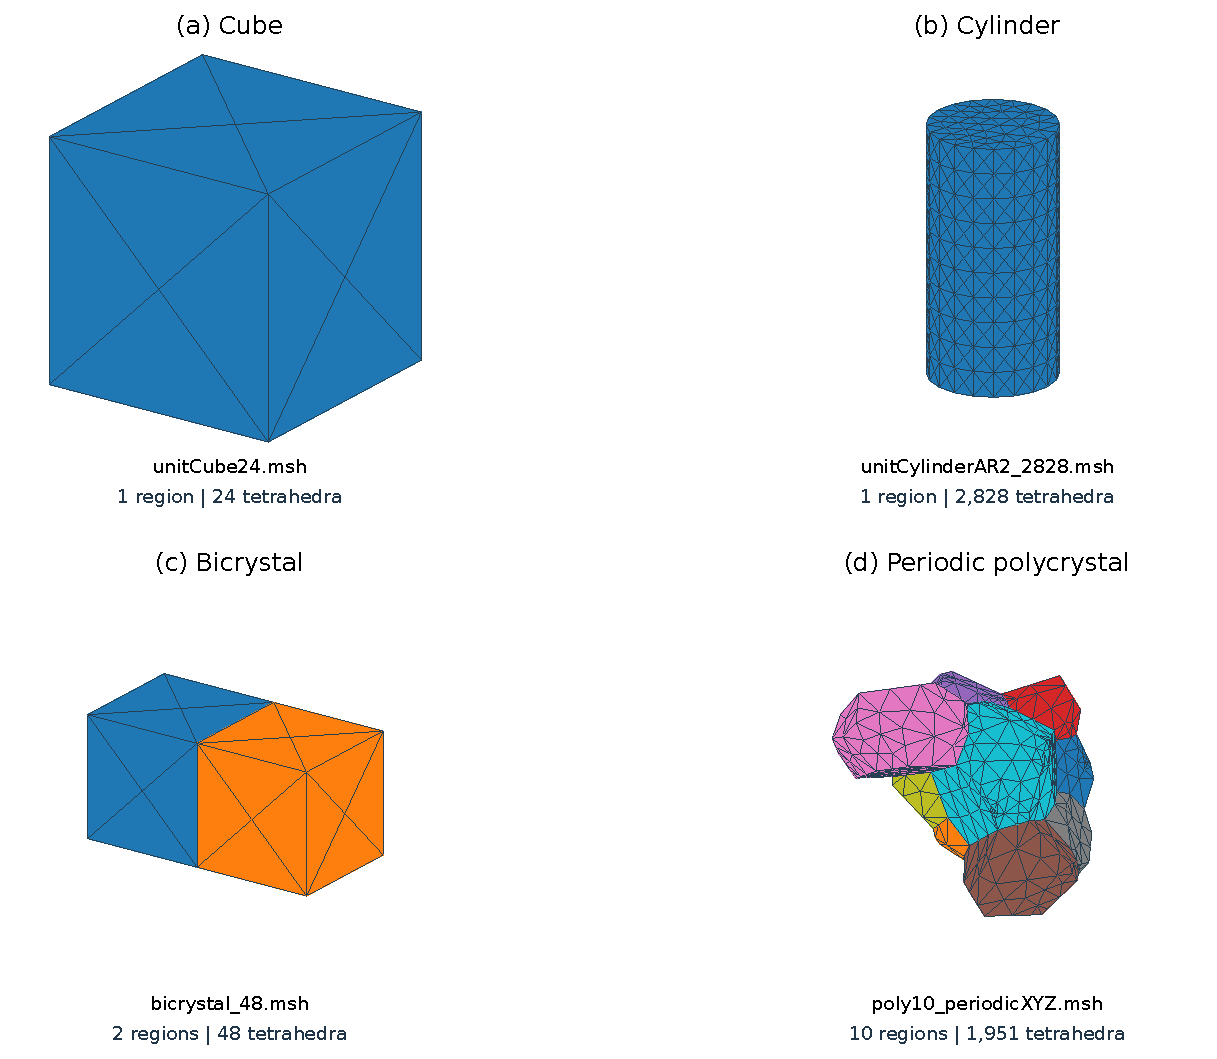
\includegraphics[width=0.98\textwidth]{mesh_library_examples}
\caption{Existing volume meshes in \code{Library/Meshes}, displayed through their exterior triangulations. Colors identify region IDs. Each specimen is scaled independently for display; counts refer to volume tetrahedra. Quadratic edge nodes, when present in the source file, are omitted from the sketches.}\label{fig:meshLibrary}
\end{figure}
Further examples include \code{polycrystalCube_10_periodicX.msh}, \code{polycrystalCube_10_periodicXY.msh}, \code{poly30_periodicXYZ.msh} and \code{polycrystalCyl_50.msh}. Select a file with the geometry, grain structure and matching periodic boundaries required by the problem, then check its region IDs against the material input.
\sourcefile{src/Mesh/SimplexReader.cpp}


\clearpage
\section{MoDELib mesh architecture}\label{sec:meshArchitecture}
The \code{.msh} mesh files are the input to the MoDELib mesh representation. The mesh constructor reads coordinates and connectivity, applies the prescribed transformation, and inserts the volume elements.

\subsection{Constructing a mesh from a file}
Both examples load \code{mesh.msh} from the working directory with the identity transformation, zero origin shift and no periodic face pairing. The coordinates are mapped as $\bm x=\bm F(\bm X-\bm x_0)$. Replace the filename with your mesh path. C++ requires MoDELib's include and link settings; Python requires NumPy and an importable \code{pyMoDELib} module.

\noindent\begin{minipage}{\linewidth}
\begin{minipage}[t]{0.48\linewidth}
\begin{tcolorbox}[enhanced,colback=manualblue!5,colframe=manualblue!35,boxrule=0.4pt,
 arc=1mm,left=2mm,right=2mm,top=7mm,bottom=2mm,height=5cm,
 overlay={\node[anchor=north east,inner sep=1mm] at (frame.north east) {\cppsymbol};}]
\begin{lstlisting}[language=C++,basicstyle=\footnotesize\ttfamily,frame=none,backgroundcolor=\color{manualblue!5},aboveskip=0pt,belowskip=0pt]
#include <MeshModule.h>

int main()
{
    Eigen::Matrix3d F = // deformation gradient
        Eigen::Matrix3d::Identity();
    Eigen::Vector3d x0 = // origin shift
        Eigen::Vector3d::Zero();

    model::SimplicialMesh<3> mesh(
        "mesh.msh", F, x0, {});
}
\end{lstlisting}
\end{tcolorbox}
\end{minipage}\hfill
\begin{minipage}[t]{0.48\linewidth}
\begin{tcolorbox}[enhanced,colback=Goldenrod!9,colframe=Goldenrod!55!black,boxrule=0.4pt,
 arc=1mm,left=2mm,right=2mm,top=7mm,bottom=2mm,height=5cm,
 overlay={\node[anchor=north east,inner sep=2mm] at (frame.north east) {\pythonsymbol};}]
\begin{lstlisting}[language=Python,basicstyle=\footnotesize\ttfamily,frame=none,backgroundcolor=\color{Goldenrod!9},aboveskip=0pt,belowskip=0pt]
import numpy as np
import pyMoDELib

F = np.eye(3)     # deformation gradient
x0 = np.zeros(3)  # origin shift

mesh = pyMoDELib.SimplicialMesh3(
    "mesh.msh", A=F, x0=x0,
    periodicFaceIDs=set()
)
\end{lstlisting}
\end{tcolorbox}
\end{minipage}
\captionsetup{hypcap=false}
\captionof{lstlisting}{Creating a mesh.}
\end{minipage}
\sourcefile{tools/pyMoDELib/MeshBindingsImplementation.h}


\subsection{Simplicial and polyhedral representations}
MoDELib implements both a discretization of the material volume and a description of its boundary topology:
\begin{itemize}
\item \code{SimplicialMesh<dim>} stores volume simplices and their lower-dimensional children. In three dimensions, these are tetrahedra, triangles, edges and vertices. It provides global point search functions and supports the finite-element architecture described in Section~\ref{sec:femArchitecture}.
\item \code{PolyhedralMesh<dim>} stores a cell complex of the grains: regions, planar faces, perimeter edges and vertices. It supports oriented boundary traversal and plane sections.

A polyhedral region is a grain-shaped volume bounded by faces. Similarly, a polyhedral face may contain many triangular mesh faces. Internal triangulation edges are absent from its perimeter, while subdivisions of the perimeter, including collinear mesh vertices, are retained.
\end{itemize}

The two representations therefore share geometry without assigning the same meaning to every edge or face.
\begin{figure}[t]
\centering
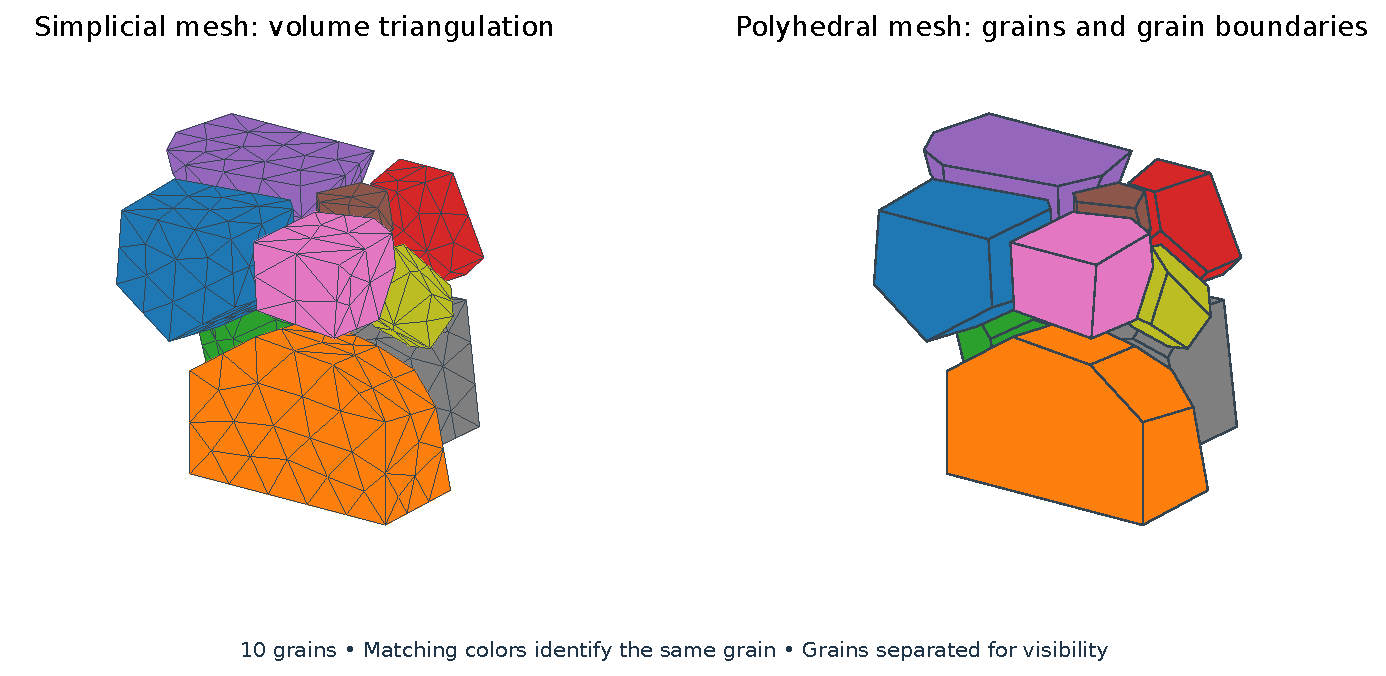
\includegraphics[width=0.80\textwidth]{polycrystal_mesh_views}
\caption{Two views of the ten-grain mesh \code{Library/Meshes/polycrystalCube_10_periodicX.msh}, containing 1081 tetrahedra. Left: the boundary triangulation of each grain, shown using tetrahedron corner vertices; quadratic edge nodes are omitted. Right: the same grain faces with internal coplanar triangle edges suppressed. Colors identify corresponding grains. Grains are separated only for visualization, exposing internal interfaces.}
\end{figure}
\sourcefile{include/Mesh/SimplicialMesh.h}
\sourcefile{include/Mesh/PolyhedralMesh.h}

\section{Simplices and shared topology}
A \code{Simplex<dim,order>} represents a simplex of topological dimension \code{order}. Vertex IDs define its identity; adjacent higher-order simplices share lower-order entities. The mesh indexes entities through one \code{SimplexFactory<dim,order>} per order, accessed with \code{simplexFactory<order>()}. The factory canonicalizes the vertex-ID key and reuses an existing simplex through \code{getOrCreate}; the same volume simplex cannot be assigned to two regions.

The mesh's \code{simplices()} map owns the volume simplices. Each simplex owns its children through shared pointers, while child-to-parent links and factory entries are weak pointers. \code{liveSimplices()} returns a map of shared pointers to the currently live entities; \code{parents()} similarly returns a temporary map of live parents. Use these views for traversal rather than treating raw factory entries as owning pointers. \code{pruneExpired()} removes expired factory entries. Keep the mesh alive while using its entities, since they also refer to mesh-owned geometry and factories.
\sourcefile{include/Mesh/SimplexFactory.h}
\sourcefile{include/Mesh/SimplexChild.h}
\sourcefile{include/Mesh/SimplexParent.h}
\manualfigure{simplex_complex}{0.98}{The simplex hierarchy in three dimensions. Arrows lead to lower-dimensional boundary entities; orange highlights a selected child in each sketch. Dashed lines show the tetrahedron's hidden edges.}

For a point $\bm x$, a tetrahedron's barycentric coordinates satisfy
\begin{equation}
\bm x=\sum_{a=0}^{3}\lambda_a\bm X_a,\qquad
\sum_{a=0}^{3}\lambda_a=1.
\end{equation}
Nonnegative coordinates characterize containment, up to numerical tolerance. The C++ search routines return a success flag and a simplex pointer. Check the flag before using the pointer as a containing element. \code{searchWithGuess} permits reuse of a nearby element, while \code{searchRegion} and \code{searchRegionWithGuess} restrict the search to a grain. This distinction is important near an interface, where geometry alone does not select a unique crystal orientation. In Python, \code{mesh.search(point)} returns the containing simplex on success and \code{None} on failure; it does not return the C++ pair.
\sourcefile{src/Mesh/SimplicialMesh.cpp}

\section{Polyhedral cells and oriented incidence}
\code{Polyhedron<dim,order>} is the common cell type. In three dimensions, a region is order 3, a face order 2, an edge order 1 and a vertex order 0. One factory per order provides shared entities keyed by IDs. Regions and faces use scalar region and face IDs as keys; lower-dimensional boundary cells are keyed by their vertex IDs.

Region cells, \code{Polyhedron<dim,dim>}, group volume simplices by region ID. A boundary between two regions is represented by \code{MeshRegionBoundary}; its planar pieces are codimension-one \code{Polyhedron<dim,dim-1>} objects.

The mesh constructor then constructs region boundaries, updates regions and their planar faces in the shared polyhedral factories, completes their boundary topology, and finally identifies active periodic face pairs. This order matters: periodic matching operates on completed external faces, and downstream consumers must see a consistent topology.

Children are held by shared pointers and parents by weak pointers. This allows a face to belong to two regions, or an edge to several faces, without creating parent--child ownership cycles. Each cell also stores its associated simplices. Codimension-one cells carry face normals, centers, region IDs and periodic partners directly. This unified representation replaces the earlier separate \code{MeshRegion} and \code{PlanarMeshFace} classes in the current mesh refactor. In 3D, a face with one incident region is external; a face with two incident regions separates grains.
\manualfigure{cell_complex}{0.98}{Geometric entities of the polyhedral complex in three dimensions. Orange highlights a selected child in each sketch. Blue arrows point to children (shared ownership); orange arrows point to parents (weak references). A face can belong to two regions. The polygonal prism is illustrative; grains may have more general shapes.}

An edge itself has no single orientation valid for every face. \code{PolyhedralFaceIncidence} supplies the orientation of that edge within one face perimeter through its \code{reversed} flag and perimeter index. \code{source()}, \code{sink()} and \code{tangent()} use that orientation. \code{next()} and \code{prev()} traverse the same perimeter; in 3D, \code{otherFace(regionID)} crosses the edge to the adjacent face bounding the specified region. Specifying the region is essential at a grain junction, where an edge can have more than two parent faces.

The constructor derives boundaries by counting simplex incidences. A boundary sub-simplex occurs once; an internal one occurs twice. Validation rejects duplicate or non-manifold input, branched or disconnected edges, and open, repeated or multiple polygon perimeters. The current polygon representation requires one closed perimeter per 2-cell; do not assume support for a face with holes. Normal orientation and grain-shell checks have a specialized 3D implementation.
\sourcefile{include/Mesh/PolyhedralMeshImplementation.h}
\sourcefile{src/Mesh/PolyhedralMesh.cpp}

\section{Mesh access from Python}
The bindings expose \code{SimplicialMesh1}, \code{SimplicialMesh2} and \code{SimplicialMesh3}, with corresponding \code{SimplexReader1/2/3} and \code{PolyhedralMesh1/2/3} types. \code{SimplicialMesh} and \code{SimplexReader} remain aliases for the three-dimensional types. Entity names encode dimension and order: for example, \code{Simplex32} is a triangular simplex in 3D and \code{Polyhedron32} is a polyhedral face in 3D. The older \code{Polyhedron0/1/2/3} names alias the corresponding 3D entities.

The Python mesh constructor accepts \code{filename}, \code{A}, \code{x0} and \code{periodicFaceIDs}. The last three arguments default to the identity matrix, zero vector and empty set, so \code{SimplicialMesh3("mesh.msh")} is sufficient for an untransformed, nonperiodic mesh. A \code{SimplexReader3} can instead read coordinates and connectivity without constructing mesh topology: \code{reader.read(filename)}, \code{reader.nodes()} and \code{reader.elements()} expose node positions and element records, where an element record is a pair of vertex IDs and region ID.

\begin{center}
\small
\begin{tabular}{p{0.36\linewidth}p{0.57\linewidth}}
\toprule
Python access & Result or use \\
\midrule
\code{mesh.simplices(order)} & Dictionary keyed by vertex-ID tuples; default order is the spatial dimension. \\
\code{mesh.polyhedralMesh()} & Derived polyhedral complex; use \code{cells(order)}, \code{region(id)}, \code{face(id)} and \code{validate()}. \\
\code{mesh.regions()}, \code{mesh.region(id)} & Region dictionary or one grain-shaped cell. \\
\code{simplex.children()}, \code{simplex.parents()} & Child list and live-parent dictionary, where the respective orders exist. \\
\code{cell.children}, \code{cell.parents} & Polyhedral child and live-parent dictionaries exposed as properties. \\
\code{cell.simplices()}, \code{cell.simplexIDs()} & Associated simplex objects or their vertex-ID tuples. \\
\code{simplex.vertices()} & Vertex objects with coordinates in \code{P0}; polyhedral vertices use \code{position}. \\
\bottomrule
\end{tabular}
\end{center}
The dictionaries are snapshots of the current entity maps, not mutable topology containers. Both \code{simplices(order)} and \code{cells(order)} reject orders outside $0,\ldots,\mathrm{dim}$. A polyhedral region provides \code{faces()}; a face provides \code{regionIDs}, \code{center()}, \code{isExternal()} and \code{outNormal(regionID)}. Positive-order simplices provide \code{bary2pos()} and \code{vertexPositionMatrix()}; volume simplices also provide \code{pos2bary()} and their \code{region}.

The following examples continue from the nonempty 3D mesh constructed above. They retrieve triangular simplices and polyhedral faces, then locate the center of a known volume simplex.
\begin{figure}[t]
\begin{minipage}[t]{0.48\linewidth}
\begin{tcolorbox}[enhanced,colback=manualblue!5,colframe=manualblue!35,boxrule=0.4pt,
 arc=1mm,left=2mm,right=2mm,top=7mm,bottom=2mm,height=6cm,
 overlay={\node[anchor=north east,inner sep=1mm] at (frame.north east) {\cppsymbol};}]
\begin{lstlisting}[language=C++,basicstyle=\footnotesize\ttfamily,frame=none,backgroundcolor=\color{manualblue!5},aboveskip=0pt,belowskip=0pt]
auto triangles =
    mesh.simplexFactory<2>()
        .liveSimplices();
const auto& poly =
    mesh.polyhedralMesh();
const auto& faces = poly.factory<2>();
poly.validate();

auto tet = mesh.simplices()
    .begin()->second;
const auto x = tet->center().eval();
auto [found, hit] = mesh.search(x);
if (found) {
    auto bary = hit->pos2bary(x);
}
\end{lstlisting}
\end{tcolorbox}
\end{minipage}\hfill
\begin{minipage}[t]{0.48\linewidth}
\begin{tcolorbox}[enhanced,colback=Goldenrod!9,colframe=Goldenrod!55!black,boxrule=0.4pt,
 arc=1mm,left=2mm,right=2mm,top=7mm,bottom=2mm,height=6cm,
 overlay={\node[anchor=north east,inner sep=2mm] at (frame.north east) {\pythonsymbol};}]
\begin{lstlisting}[language=Python,basicstyle=\footnotesize\ttfamily,frame=none,backgroundcolor=\color{Goldenrod!9},aboveskip=0pt,belowskip=0pt]
triangles = mesh.simplices(2)
poly = mesh.polyhedralMesh()
faces = poly.cells(2)
poly.validate()

tet = next(iter(
    mesh.simplices().values()))
x = tet.center()
hit = mesh.search(x)
if hit is not None:
    bary = hit.pos2bary(x)
\end{lstlisting}
\end{tcolorbox}
\end{minipage}
\captionsetup{hypcap=false}
\captionof{lstlisting}{Inspecting mesh topology and locating a point.}
\end{figure}
\sourcefile{tools/pyMoDELib/MeshBindingsImplementation.h}

\section{Plane sections and lifetime}
\code{MeshPlane} combines a geometric plane with its intersections with the mesh. \code{BoundingMeshSegments} and \code{MeshBoundarySegment} carry the resulting boundary segments and their supporting faces. These are the geometric foundation for a glide plane clipped to a grain. A plane section must retain connectivity and face incidence; sorting all intersection points around a center is insufficient for general nonconvex domains.

\code{SimplicialMesh} owns its polyhedral complex and exposes it through \code{polyhedralMesh()}. Re-reading the mesh rebuilds this derived structure and clears periodic simplex pairs. References to old cells, faces, or finite-element data must not be reused after a rebuild. Python objects returned by mesh and connectivity queries retain the owning mesh; retaining a child therefore keeps its mesh alive without making reciprocal parent--child ownership cycles. This lifetime support does not make old entities valid after a C++ mesh rebuild. The Python interface currently exposes neither \code{readMesh} nor \code{identifyParallelFaces}; construct a new mesh to change its input or active pairing. In normal simulations, \code{DefectiveCrystalBase} supplies shared ownership of the mesh to consumers and treats the geometry as fixed.
\sourcefile{include/Mesh/MeshPlane.h}
\sourcefile{src/Mesh/MeshBoundarySegment.cpp}

\section{Preparing and checking a mesh}
The simulation's \code{inputFiles/polycrystal.txt} selects \code{meshFile}. Paths are resolved relative to \code{inputFiles/}. The matrix \code{F} and vector \code{X0} transform the input coordinates as $\bm x=\bm F(\bm X-\bm X_0)$; \code{X0} is subtracted before applying \code{F}. This is a mesh placement/scaling operation, not the evolving elastic deformation. Coordinates used internally are in Burgers-vector units. Region IDs must agree with the grain rotations described in Chapter~\ref{chap:materials}.

Before a run, check that the mesh is nonempty, the intended region IDs exist, and periodic partners have matching translated triangulations. The repository tests \code{testPolyhedralMesh.cpp}, \code{testPolyhedralMeshDimensions.cpp}, \code{testPlaneSectionMesh.cpp} and \code{testNonconvexMeshSearch.cpp} exercise different parts of these contracts. \code{testPythonMesh.py} additionally checks the bindings across dimensions 1--3, including connectivity, periodic pairing and ownership. The C++ tests identify verification entry points; this documentation update does not report a new execution of those tests.
\sourcefile{include/Mesh/Polyhedron.h}
\sourcefile{src/Mesh/GmshReader.cpp}

\section{Geometric periodicity}\label{sec:periodicity}
\subsection{The translation lattice}
Periodicity identifies points separated by integer combinations of active translation vectors. Let $\bm A=[\bm a_1\ \cdots\ \bm a_p]$ contain a basis of the periodic directions, with $0\le p\le3$. Equivalent points obey
\begin{equation}
\bm x' = \bm x+\bm A\bm n,\qquad \bm n\in\mathbb Z^p.
\end{equation}
Partial periodicity means $p<3$: unpaired external faces remain physical boundaries. The basis need not coincide with the Cartesian axes. \code{DefectiveCrystalBase} stores the basis and its dual
\begin{equation}
\bm A^*=\bm A(\bm A^T\bm A)^{-1},\qquad
\bm\xi=(\bm A^*)^T(\bm x-\bm x_c),
\end{equation}
where $\bm x_c$ is the mesh bounding-box center. There is no $2\pi$ factor in this coordinate dual. For partial periodicity, $\bm\xi$ records only the coordinates along the periodic span.
\manualfigure{periodicity}{0.98}{(a) An oblique translation lattice and equivalent points. (b) A two-dimensional polycrystal unit at the origin, composed of whole grains with a jagged outer boundary along grain boundaries. (c) Translations of this same jagged unit tile the plane without cutting grains at a lattice parallelogram. Opacity decreases with distance from the origin only for visual clarity; the polycrystal is schematic.}

\subsection{Selecting and matching faces}
The mesh constructor accepts a set of \code{periodicFaceIDs}. An empty set disables pairing; \code{-1} enables all valid discovered periodic directions. Explicit values select external planar face IDs. These are MoDELib face IDs, not automatically Gmsh physical surface tags, so inspect the mesh's face numbering before selecting a subset.

\code{identifyParallelFaces} first discovers a valid full lattice and then selects the active lattice. A face pair must match under a translation, including its boundary simplex connectivity. Parallel normals alone are insufficient. Only pairs whose shifts are integer combinations of the selected lattice are activated. The mesh records both the planar-face relation and a \code{PeriodicSimplexPair} for each paired boundary simplex.

A simplex pair stores the partner pointer, the shift with convention
\begin{equation}
\bm x_{\mathrm{partner}}=\bm x_{\mathrm{source}}+\bm s,
\end{equation}
and the permutation matching source vertices to partner vertices. The reverse relation must have the opposite shift and inverse permutation. Pairing is committed only after these checks succeed. This makes all subsequent users consume the same geometric correspondence.
If pairing fails, check translated boundary nodes, triangulation and selected face IDs. Field constraints are described in Section~\ref{sec:periodicFEM}.
\sourcefile{include/Mesh/PeriodicMeshFacePairing.h}
\sourcefile{include/Mesh/PeriodicSimplexPair.h}
\sourcefile{src/Mesh/SimplicialMesh.cpp}



\chapter{Materials and polycrystals}\label{chap:materials}
\section{Shared material, grain-specific crystallography}
\code{PolycrystallineMaterialBase} reads the material identity, crystal structure, temperature-dependent scales, elastic constants, enabled slip systems and second phases. \code{Polycrystal<3>} combines this shared material with the mesh's collection of grains. Each mesh region produces a \code{Grain}; each grain derives from \code{SingleCrystalBase}, which provides its oriented lattice, plane normals, slip systems and second phases.

In this design, changing a grain's orientation changes its crystallography while the material scale is shared. A collection of differently oriented grains is therefore not, by itself, a collection of different material files. The current base reads one material file for the polycrystal and checks that grains have a common atomic volume.
\manualfigure{polycrystal}{0.98}{Construction of the polycrystal. Geometry provides the regions, the shared material provides constitutive data, and a rotation supplies each grain's crystallographic orientation.}
\sourcefile{src/PolycrystallineMaterials/PolycrystallineMaterialBase.cpp}
\sourcefile{src/PolycrystallineMaterials/Polycrystal.cpp}

\section{Units and temperature}
The fundamental scales are the Burgers-vector magnitude $b_{\mathrm{SI}}$, the shear modulus $\mu_{\mathrm{SI}}$, and the shear-wave speed $c_{s,\mathrm{SI}}$. The current material constructor uses
\begin{equation}
\mu_{\mathrm{SI}}(T)=\mu_{0,\mathrm{SI}}+\mu_{1,\mathrm{SI}}T,
\quad c_{s,\mathrm{SI}}=\sqrt{\mu_{\mathrm{SI}}/\rho_{\mathrm{SI}}},
\quad E_{\mathrm{SI}}=2\mu_{\mathrm{SI}}(1+\nu).
\end{equation}
Internal values of $b$, $\mu$ and $c_s$ are one. To interpret outputs, use
\begin{center}
\begin{tabular}{lll}\toprule
Quantity & Internal value & SI conversion\\\midrule
Position & $\hat x$ & $b_{\mathrm{SI}}\hat x$\\
Time & $\hat t$ & $(b_{\mathrm{SI}}/c_{s,\mathrm{SI}})\hat t$\\
Velocity & $\hat v$ & $c_{s,\mathrm{SI}}\hat v$\\
Stress & $\hat\sigma$ & $\mu_{\mathrm{SI}}\hat\sigma$\\
Energy & $\hat E$ & $\mu_{\mathrm{SI}}b_{\mathrm{SI}}^3\hat E$\\\bottomrule
\end{tabular}
\end{center}
A physical length used to scale a unit mesh must be divided by $b_{\mathrm{SI}}$. Input names ending in \code{_SI}, or naming units such as \code{_eV}, identify dimensional values; other controls must be checked in their template. Temperature is in kelvin.

The presence of crystallographic anisotropy in slip systems does not imply that every elastic solver uses an anisotropic stiffness. The current elastic-deformation module constructs isotropic stiffness from $\mu$ and $\nu$. The anisotropic dislocation derivations retained later in the manual are general theory and should not be read as a statement that every runtime kernel implements that generality.

\section{Grains, rotations and boundaries}
For each region ID $r$, \code{Grain} reads the crystal to global (\code{C2G}) transformation matrix from the entry named \code{C2G} followed by that ID, for example \code{C2G1}. This matrix maps crystal coordinates to global coordinates. For a proper rotation $\bm Q$, a crystal vector transforms as $\bm v_g=\bm Q\bm v_c$, and a second-order tensor as $\bm T_g=\bm Q\bm T_c\bm Q^T$. Use orthogonal matrices with determinant $+1$; a mesh scaling belongs in \code{F}, not in the crystal rotation.

\code{SingleCrystalSelector} chooses the lattice and available crystallographic objects from the material's crystal structure. \code{enabledSlipSystems} selects which systems are constructed. A slip system combines a slip direction, plane and mobility behavior; material mobility data must be compatible with the selected systems. Grain boundaries associate neighboring grains with their geometric region boundary and planar face. Their existence as objects does not automatically supply a constitutive rule for transmission of dislocations.
\sourcefile{src/PolycrystallineMaterials/Grain.cpp}
\sourcefile{include/PolycrystallineMaterials/SingleCrystalBase.h}
\sourcefile{include/PolycrystallineMaterials/GrainBoundary.h}

\section{Input workflow}
Copy a material file from \code{Library/Materials/} to the simulation's \code{inputFiles/}. Select it in \code{polycrystal.txt} alongside the mesh and temperature. Supply a rotation for every mesh region, using the actual region IDs rather than assuming consecutive numbering.
\par\noindent\begin{minipage}{\linewidth}
\begin{lstlisting}
# Illustrative polycrystal fragment: filenames must exist locally.
materialFile=W.txt;
meshFile=unitCube24.msh;
absoluteTemperature=300;
F=1000 0 0
  0 1000 0
  0 0 1000;
X0=0 0 0;
C2G1=1 0 0
     0 1 0
     0 0 1;
periodicFaceIDs=-1;
\end{lstlisting}
\end{minipage}\par
This example scales a unit cube to side length $1000b$. It is a geometry/material fragment, not a complete simulation. For a multigrain mesh, add the corresponding \code{C2G} entries. The tutorial helper \code{PolyCrystalFile} is useful for generating single-grain input; inspect its output before extending it to several grains.

A source-level material investigation should follow the reading class: basic elastic scales in \code{PolycrystallineMaterialBase}, slip-system construction in the crystal-specific classes, mobility in \code{DislocationMobilities}, and diffusion/reaction parameters in the CD context. This avoids treating one material file as a single constitutive law.

\chapter{Finite-element infrastructure}\label{chap:fem}
\section{Geometry, interpolation and fields}\label{sec:femArchitecture}
The volume mesh is geometry. \code{FiniteElement<ElementType>} adds interpolation nodes and elements. \code{TrialFunction} carries a field's unknowns and conditions; differential operators and integration domains build weak forms; \code{WeakProblem} assembles and solves the constrained system. Keeping these roles separate allows multiple physics to reuse the same geometric discretization while defining different fields and equations.

The current \code{DefectiveCrystalBase::ElementType} is \code{LagrangeElement<3,2>}: quadratic tetrahedra. A tetrahedron therefore has ten interpolation nodes, including its edge midpoints, even if the source Gmsh mesh supplies only the four vertices of each volume element. A vector displacement has three components per interpolation node; concentrations have their own component counts.
\manualfigure{fem}{0.98}{Left: the three analytical quadratic Lagrange functions along an element edge. Their midpoint degree of freedom explains why vertex-only periodic matching is insufficient. Right: the responsibility chain from geometry to a constrained solve.}
\sourcefile{include/FEM/FiniteElement.h}
\sourcefile{include/FEM/LagrangeElement.h}
\sourcefile{include/FEM/TrialFunction.h}

\section{The weak-form contract}
For illustration, small-strain elasticity uses $\bm\varepsilon(\bm u)=\operatorname{sym}\nabla\bm u$. Its bilinear form is
\begin{equation}
a(\bm v,\bm u)=\int_\Omega\bm\varepsilon(\bm v):\mathbb C:\bm\varepsilon(\bm u)\dV.
\end{equation}
The elastic module builds the corresponding expression with \code{def(u)}, a stiffness multiplication, a test function and a volume domain. This expression describes a mathematical operator; boundary conditions, affine modes and rigid-motion control are supplied separately. The right-hand side depends on the physics, external loading and coupling fields.

\paragraph{Solve a clamped elasticity problem.}
The following C++ function accepts a shared, nonperiodic mesh of a connected block with a planar $x=x_{\min}$ face. It clamps all displacement components on that face, applies a constant body force, and leaves the other faces traction-free. The example uses $\mu=1$ and $\nu=0.3$ in consistent units. The returned vector contains the solved nodal displacements. The weak-form API used here is not currently exposed by \code{pyMoDELib}.

\begin{figure}[htbp]
\begin{tcolorbox}[enhanced,colback=manualblue!5,colframe=manualblue!35,boxrule=0.4pt,
 arc=1mm,left=2mm,right=2mm,top=7mm,bottom=2mm,
 overlay={\node[anchor=north east,inner sep=1mm] at (frame.north east) {\cppsymbol};}]
\lstinputlisting[language=C++,basicstyle=\footnotesize\ttfamily,frame=none,backgroundcolor=\color{manualblue!5},aboveskip=0pt,belowskip=0pt]{tex/snippets/elasticity.cpp}
\end{tcolorbox}
\captionsetup{hypcap=false}
\captionof{lstlisting}{Solving linear elasticity with a clamped face and a body force.}
\end{figure}

For a discrete linear system $\bm K\bm u=\bm f$, constraint elimination can be understood through $\bm u=\bm P\bm q+\bm c$:
\begin{equation}
\bm P^T\bm K\bm P\bm q=\bm P^T(\bm f-\bm K\bm c).
\end{equation}
This is a conceptual reduction, not an assertion that every solve uses only this equation: \code{WeakProblem} also supports global linear constraints and additional affine modes. Its checks detect incompatible prescribed values and invalid constraint systems, and verify residuals after solving.
\sourcefile{include/FEM/WeakProblem.h}
\sourcefile{src/ElasticDeformation/ElasticDeformationFEM.cpp}

\section{Periodic equivalence classes and field constraints}\label{sec:periodicFEM}
\code{PeriodicFEMNodePairing} extends boundary-simplex correspondence to finite-element nodes using their barycentric integer indices. This includes higher-order edge and face nodes, not only mesh vertices. A graph traversal constructs a representative node and translation for every equivalence class. Cycles at edges and corners must give consistent total shifts.

The pairing object records geometry; the weak-problem solver uses it to constrain field degrees of freedom. For an affine-periodic vector field,
\begin{equation}\label{eq:affineperiodic}
\bm u_i=\bm u_{r(i)}+\bm H\bm s_i+\bm q_i-\bm q_{r(i)},
\end{equation}
where $r(i)$ is the representative, $\bm s_i$ the geometric shift, $\bm H$ the prescribed field gradient, and $\bm q$ an optional nodal offset. Zero gradient and zero offset give a strictly periodic field. Global affine modes may also be solved as unknowns by the loading controller. Incompatible nodal Dirichlet values and affine/periodic conditions are rejected rather than silently overwritten.

Continuous finite-element spaces acquire periodic node relations. Discontinuous spaces retain independent nodes. If active mesh pairing is changed after finite-element construction, explicitly rebuild the periodic node pairing before constructing or solving dependent fields.
\sourcefile{include/FEM/PeriodicFEMNodePairing.h}
\sourcefile{include/FEM/FiniteElement.h}
\sourcefile{include/FEM/WeakProblem.h}

\manualfigure{affine_periodic_field}{0.65}{An affine-periodic field $u(x)=0.5x+0.12\sin(2\pi x)$ combines an affine jump with a periodic fluctuation. These analytical curves illustrate field constraints; they are not solver output.}

If a solve rejects constraints, inspect prescribed values on every copy of an equivalence class. Relevant checks include \code{testPeriodicFEMNodes.cpp}.

\section{Physical boundaries and rigid modes}
Equation~\eqref{eq:affineperiodic} expresses the relationship between equivalent field nodes. The finite-element pairing supplies representatives and shifts, while the field supplies its gradient and optional offset. This distinction allows the same periodic mesh to host different fields.

A paired external face is not a free surface. \code{NonPeriodicExternalBoundary} excludes paired boundary simplices from the physical-boundary integration domain. For elastic loading, periodic directions can carry free affine jumps determined by the controller, while physical faces receive the associated traction. Applying a free-surface load to both members of a periodic pair would count a boundary that has already been identified internally.

Elasticity also has rigid-motion null modes. The elastic module uses \code{GlobalRigidMotionPenalty} to control admissible mean displacement and mean infinitesimal rotation globally. Its weight is \code{inertiaReliefPenaltyFactor}. This is a global reference condition; it is not an arbitrary clamp on a chosen mesh vertex.
\sourcefile{include/FEM/NonPeriodicExternalBoundary.h}
\sourcefile{src/ElasticDeformation/ElasticDeformation.cpp}

\section{Enabling and diagnosing FEM}
\code{useFEM} in \code{DefectiveCrystal.txt} creates the shared finite-element infrastructure. \code{useElasticDeformationFEM} in \code{ElasticDeformation.txt} selects the elastic module's FEM formulation. They have different roles: enabling the shared FEM does not itself choose elastic-deformation physics. Conversely, a physics needing the FEM cannot work with that infrastructure disabled.

For an elastic FEM run, select \code{ElasticDeformation} in \code{physics}, set \code{useFEM=1}, and set \code{useElasticDeformationFEM=1}. Keep the material, boundary pairing, and loading choices consistent. On a failed solve, inspect constraints and null modes before changing numerical tolerances. On a periodic mismatch, verify higher-order nodes as well as mesh vertices. For accuracy, compare an observable under mesh refinement; the polynomial order alone is not an accuracy certificate.

\part{Multiphysics and shared field physics}
\chapter{The multiphysics architecture}\label{chap:multiphysics}
\section{Shared context and evolving state}
\code{DefectiveCrystalBase} constructs the simulation context: parameters and paths, shared mesh ownership, periodic translations, shared polycrystal ownership, optional finite elements, and the base contexts of enabled physics. It also serves microstructure generation. \code{DefectiveCrystal} creates the selected evolving microstructures and advances the simulation.

\code{MicrostructureBase} is the interface each physics implements. \code{MicrostructureContainer} is both a collection of these objects and an implementation of the same interface. Thus the container can forward lifecycle operations and expose aggregate fields without requiring callers to know the concrete type of every physics.
\begin{figure}[htbp]
\centering
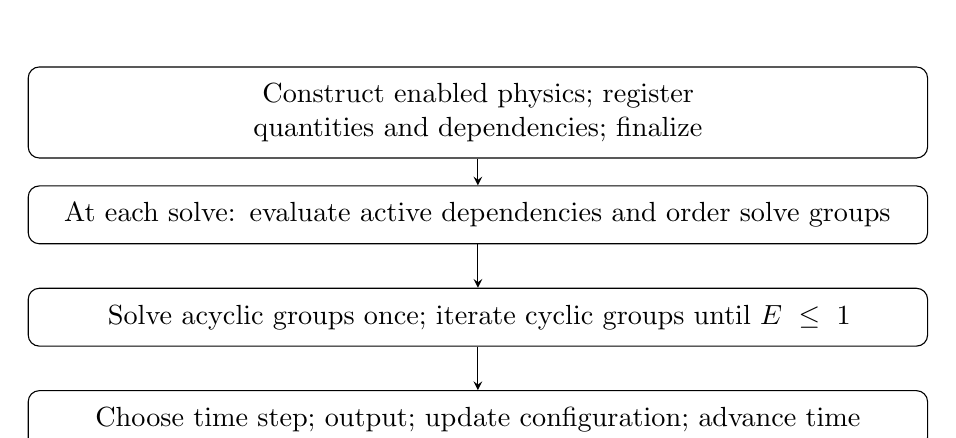
\begin{tikzpicture}[every node/.style={draw,rounded corners,align=center,text width=11cm,inner sep=6pt},>=stealth]
\node (registration) at (0,0) {Construct enabled physics; register quantities and dependencies; finalize};
\node (groups) at (0,-1.3) {At each solve: evaluate active dependencies and order solve groups};
\node (solve) at (0,-2.6) {Solve acyclic groups once; iterate cyclic groups until $E\leq1$};
\node (advance) at (0,-3.9) {Choose time step; output; update configuration; advance time};
\draw[->] (registration) -- (groups);
\draw[->] (groups) -- (solve);
\draw[->] (solve) -- (advance);
\end{tikzpicture}
\caption{Dependency-based multiphysics solution. Geometry and time remain fixed during the solve groups.}
\end{figure}
\sourcefile{include/DefectiveCrystal/DefectiveCrystalBase.h}
\sourcefile{include/DefectiveCrystal/MicrostructureBase.h}
\sourcefile{src/DefectiveCrystal/MicrostructureContainer.cpp}

\section{Lifecycle and common field queries}
The interface includes initialization from a configuration, \code{solve()}, \code{getDt()}, \code{output()} and \code{updateConfiguration()}. It also exposes stress, displacement, inelastic displacement rate, mobile concentrations, immobile clusters, and volume-average quantities. A physics contributes the quantities it represents and returns the appropriate zero contribution for others.

The container sums returned fields. For example,
\begin{equation}
\bm\sigma(\bm x)=\sum_\alpha\bm\sigma^{(\alpha)}(\bm x),\qquad
\langle\bm\beta^P\rangle=\sum_\alpha\langle\bm\beta^{P,(\alpha)}\rangle.
\end{equation}
This additive interface makes coupling accessible, but the module must still define which part of the field it owns. In particular, an elastic correction must not double-count a dislocation's analytical stress. The optional node, element and simplex arguments of field queries provide geometric context and can avoid redundant searches.

\section{Solved quantities and solve groups}\label{sec:solvedQuantities}
The solution order is determined by dependencies between quantities, rather than by the order of physics names in the input. \code{MicrostructureContainer} owns a \code{SolvedQuantityRegistry} and its ordered \code{SolvedQuantityGroup} objects. After constructing all enabled physics, \code{DefectiveCrystal} explicitly calls \code{finalizeSolvedQuantities()}. Each physics registers its operations through \code{registerSolvedQuantities()}.

A \code{SolvedQuantityContribution} describes one update operation: its provider and name, the quantities it publishes, the quantities it needs, and its update callback. One operation can publish several quantities. For example, the DD velocity operation also publishes the dislocation contribution to mobile concentration. Dependencies can select all other providers of a quantity or a particular named provider. A required dependency without a provider is an error; optional dependencies accommodate disabled physics.

At the start of each solve, the registry evaluates conditional dependencies and constructs the directed dependency graph. It finds strongly connected components and orders them so that prerequisites are available first. An acyclic operation is solved once. Operations connected by a dependency cycle form a coupled group and are iterated to convergence. The graph can change between glide and climb steps: concentration feedback is active during climb, but not during glide.

Within a coupled group, operations execute sequentially in a deterministic order, using the latest available results from earlier operations in the same iteration. This is a block fixed-point iteration of Gauss--Seidel type, not a monolithic Newton solve. A group must converge before downstream groups execute.
\sourcefile{include/DefectiveCrystal/SolvedQuantityRegistry.h}
\sourcefile{src/DefectiveCrystal/SolvedQuantityRegistry.cpp}

\subsection{Example: coupled dislocation climb and diffusion}
For a DD/CD/ED climb calculation, a typical sequence is:
\begin{lstlisting}
Solve sequence (5 groups):
  Group 1 [solve once]
    DislocationDynamics:Stress
  Group 2 [solve once]
    ElasticDeformation:Stress
  Group 3 [iterate to convergence]
    ClusterDynamics:MobileConcentration
    DislocationDynamics:Velocity
  Group 4 [solve once]
    ClusterDynamics:ImmobileRates
  Group 5 [solve once]
    ElasticDeformation:DisplacementRate
\end{lstlisting}
The DD stress operation makes the geometry-dependent analytical field available; it does not solve a separate stress system. ED computes the elastic correction before the concentration--velocity iteration. CD concentrations affect climb velocities, while climb velocities affect the dislocation concentration contribution used in CD boundary conditions. These two operations therefore form a cycle. Immobile rates and inelastic displacement rates are evaluated after that cycle converges.

This is an example, not a hard-coded five-stage schedule. The enabled physics and active dependencies determine the groups. DDomp prints the sequence on the first solve and again if its structure changes, rather than repeating an unchanged sequence at every time step.

\section{Convergence control}\label{sec:coupledTolerance}
Each operation in a cyclic group supplies a state vector, a restore callback, and componentwise absolute tolerances. Let $s_j^{\mathrm{old}}$ be a component immediately before its operation and $s_j^*$ the result of that operation before relaxation. Define
\begin{align}
 d_j&=|s_j^*-s_j^{\mathrm{old}}|,\\
 \tau_j&=a_j+r\max\bigl(|s_j^{\mathrm{old}}|,|s_j^*|\bigr),\\
 E&=\max_{\text{operations and components }j}\frac{d_j}{\tau_j}.
\end{align}
The group converges when $E\leq1$ after a complete iteration. Thus every monitored component must pass; a large update cannot be hidden by averaging over many small components. This measures fixed-point consistency between physics. It is distinct from a linear solver residual, a spatial discretization error, or a time-integration error estimate.

The relative tolerance $r$ is dimensionless. When the relative term dominates, $r=10^{-3}$ permits an update of approximately $0.1\%$ of the component magnitude. The absolute tolerance $a_j$ has the units of that component and provides a floor near zero. For example, with a velocity magnitude $10^{-20}$, $r=10^{-3}$ and $a_j=10^{-24}$, the permitted update is $1.1\times10^{-23}$. An update of $2.2\times10^{-23}$ has normalized error two and fails. Larger tolerances loosen the criterion; smaller tolerances tighten it.

\subsection{Monitored states and absolute floors}
For DD, the state contains each network node's scalar climb rates for all mobile species, followed by its Cartesian velocity components. Its ordering follows the network-node container. The absolute velocity tolerance is expressed in MoDELib's internal velocity units, not directly in metres per second.

For CD, the state is the FEM mobile-concentration degree-of-freedom vector with the species' zero-stress equilibrium concentration subtracted:
\begin{equation}
 s_{n,\alpha}=c^{\mathrm{FEM}}_{n,\alpha}-c^{\mathrm{eq}}_\alpha(0),\qquad
 a_{n,\alpha}=f_{\mathrm{abs}}\max\bigl(|c^{\mathrm{eq}}_\alpha(0)|,10^{-100}\bigr).
\end{equation}
Subtracting the equilibrium background prevents a large equilibrium concentration from masking changes in the FEM correction. The absolute floor is species-dependent. The numerical floor $10^{-100}$ avoids a vanishing scale for a zero equilibrium concentration. Restoring the CD state adds the equilibrium background back before storing the complete FEM field.

\subsection{Input parameters}
The following optional settings belong in \code{inputFiles/DefectiveCrystal.txt}; the values shown are the current defaults:
\begin{lstlisting}
solvedQuantityMaxIterations=100;
solvedQuantityRelativeTolerance=1.e-3;
solvedQuantityRelaxation=1.0;
solvedQuantityVelocityAbsoluteTolerance=1.e-24;
solvedQuantityConcentrationAbsoluteFraction=1.e-10;
\end{lstlisting}
The iteration limit must be positive, the relative tolerance nonnegative, the velocity absolute tolerance and concentration fraction positive, and the relaxation factor must satisfy $0<\omega\leq1$. These inputs control the coupling iteration; they do not select the direct or iterative FEM solver or change its residual tolerance.

After measuring the unrelaxed discrepancy, the state is replaced by
\begin{equation}
 s^{\mathrm{new}}=s^{\mathrm{old}}+\omega(s^*-s^{\mathrm{old}}).
\end{equation}
With $\omega=1$ the complete update is accepted. Smaller values damp the coupling iteration and can help oscillatory fixed-point iterations, but may require more iterations. Testing the unrelaxed discrepancy prevents a small relaxation factor from creating false convergence.

\subsection{Diagnostics and failure handling}
Every coupled iteration reports its normalized error and the controlling component: \code{provider:operation}, zero-based state index, absolute update, and permitted tolerance. The index belongs to that operation's state vector; it is not a network-node ID. An error of ten means that the largest normalized update is ten times its permitted tolerance, not a ten-percent error.

If the iteration limit is reached, an update throws, or a monitored state becomes invalid, the cyclic group restores its registered states to their values at group entry and propagates the error. The time step is not advanced. This is rollback of the group's iterated fields and rates, not a snapshot of every internal object or of previously completed groups. Prepared caches may remain allocated and are refreshed at the next solve. The former \code{reSolve()} interface has been removed; ED now exposes \code{solveDisplacementRate()} for its dedicated rate operation. The former \code{maxResolveSteps} input no longer controls coupling; it is superseded by convergence-based groups.

\section{Fixed geometry and reuse within a solve}
Geometry, topology, simulation time, and immobile populations do not advance during a coupled iteration. This makes the following reuse possible:
\begin{itemize}
\item DD quadrature stresses and equilibrium concentrations remain fixed while CD concentrations and climb velocities iterate. The climb interaction matrix is prepared on the first iteration and reused subsequently.
\item CD sink equilibrium concentrations are cached within the solve. The dislocation-to-FEM influence matrices $H_\alpha$ map scalar climb velocities to nodal concentration contributions,
\begin{equation}
 \bm c^{D}_\alpha=H_\alpha\bm v^{\mathrm{climb}}_\alpha.
\end{equation}
They are built once per coupled solve, including retries, and retain the segment kernels, grain filtering, periodic images and shared network-node endpoints. Only required sink/periodic nodes are stored unless reactions need all FEM nodes. Later iterations use matrix--vector products.
\item FEM factorizations are reused while matrices and constraint structure remain unchanged. Changing boundary values or right-hand sides alone does not require refactorization.
\end{itemize}
Construction of $H_\alpha$ and sink-stress evaluations use OpenMP with independent target-node outputs. ED evaluates external surface tractions in parallel and assembles their contributions in a fixed order. These optimizations preserve the solve-group dependency order; they do not run dependent physics simultaneously.

The current graph places ED stress outside the climb--diffusion cycle. A future constitutive model whose stress depends on the iterated concentration must register that dependency and revise the cache lifetime accordingly; the current fixed-stress assumption must not be carried over silently.

\section{One simulation step}
The ordering in \code{DefectiveCrystal::runSingleStep} is:
\begin{enumerate}
\item Invoke the container's dependency-based solve and converge each cyclic group.
\item Choose $\Delta t=\min(\Delta t_{\max},\Delta t_1,\ldots,\Delta t_n)$ from the physics time-step restrictions.
\item If this is an output step, write the current configuration, auxiliary data and scalar history.
\item Call \code{updateConfiguration()} on the microstructures.
\item Advance simulation time and increment \code{runID}.
\end{enumerate}
Output therefore records the configuration before that step's update. \code{Nsteps} is the terminal step index in the run loop; after a restart it is not automatically a count of additional steps. Coupled iterations do not represent extra physical time steps.
\sourcefile{src/DefectiveCrystal/DefectiveCrystal.cpp}

\section{Selecting and extending physics}
The \code{physics} line in \code{DefectiveCrystal.txt} accepts space-separated names:
\par\noindent\begin{minipage}{\linewidth}
\begin{lstlisting}
physics=DislocationDynamics ElasticDeformation;
\end{lstlisting}
\end{minipage}\par
Available names are \code{DislocationDynamics}, \code{ElasticDeformation}, \code{InclusionMicrostructure} and \code{ClusterDynamics}. Parsing is case-insensitive and removes duplicate names while preserving order. \code{none} is a template placeholder; a run with no actual physics is rejected. The quantity dependency graph determines solve order; the physics list is not a substitute for declaring dependencies.

A new physics needs an implementation of \code{MicrostructureBase}, configuration and output support, and registration in the physics parsing and construction paths. Its field contribution and time-step restriction must be defined explicitly. Register its solved quantities and dependencies; any operation participating in a cycle must also provide state, restore and absolute-tolerance callbacks. The default compatibility adapter publishes stress and calls the existing solve once, so it is not sufficient to describe new feedback cycles. Mesh and material data should come from the shared context rather than from a second independently constructed crystal.

\chapter{Running a simulation}\label{runningMoDELib}
\section{Build the tools}
The repository uses C++20 and CMake 3.20 or later. Eigen and FFTW are required by the current build. OpenMP is used by the simulation tools. Qt/VTK are needed for the optional viewer, and pybind11 for optional Python bindings. The root \code{CMakeLists.txt} is the authoritative list of build options for this snapshot.

From the repository root, a command-line configuration is:
\par\noindent\begin{minipage}{\linewidth}
\begin{lstlisting}[language=bash]
cmake -S . -B build -DUSE_PYBIND11=OFF -DBUILD_DDQT=OFF
cmake --build build -j
\end{lstlisting}
\end{minipage}\par
This builds the simulation tools without requiring the viewer or Python bindings. Tutorial input generators still need Python and NumPy. Plotting scripts generally need Matplotlib. CD species counts are compile-time options; match them to the chosen CD material when that physics is enabled.

\section{The simulation folder}
A simulation has an \code{inputFiles/} directory, a \code{config/} directory, and an \code{F/} directory for history output. The generator writes the initial microstructure; the driver evolves it. Copy templates into the simulation before editing them.
\begin{center}\small
\begin{tabular}{p{0.35\textwidth}p{0.57\textwidth}}\toprule
File & Responsibility\\\midrule
\code{polycrystal.txt} & Mesh, transformations, temperature, material, grain orientations and periodic faces.\\
\code{DefectiveCrystal.txt} & Physics selection, shared FEM switch, time stepping, image counts and output schedule.\\
Material file & Units, elasticity, crystal structure and constitutive parameters.\\
\code{DD.txt} & DDD solver, remeshing and dislocation-specific controls.\\
\code{ElasticDeformation.txt} & Uniform/FEM elasticity, loading and rigid-motion control.\\
\code{initialMicrostructure.txt} & List of microstructure specifications consumed by the generator.\\
\code{ClusterDynamics.txt} & Current CD-specific controls, when enabled.\\\bottomrule
\end{tabular}\end{center}
Inputs generally use \code{name=value;} and \code{\#} comments. Arrays are whitespace-separated; matrices have rows and one terminating semicolon. Use the complete template for each enabled physics rather than assembling a deck from isolated examples in this manual.

\section{A first DDD run}
The \code{dipoles} tutorial demonstrates the complete path. Run in a fresh copy if that tutorial folder contains results you wish to keep. From the repository root:
\par\noindent\begin{minipage}{\linewidth}
\begin{lstlisting}[language=bash]
cd tutorials/dipoles
python3 generateInputFiles.py
../../build/tools/MicrostructureGenerator/microstructureGenerator .
../../build/tools/DDomp/DDomp .
\end{lstlisting}
\end{minipage}\par
The supplied generator selects DDD and elastic deformation, copies the material and mesh, generates \code{polycrystal.txt}, and writes the microstructure specifications. Its default is a long run. For an initial check, edit the generated \code{DefectiveCrystal.txt} to set \code{Nsteps=2;} and \code{outputFrequency=1;} before invoking \code{DDomp}. The commands here document the workflow; no simulation was run as part of this manual revision.

\section{Outputs and restart}
\code{config/evl_*.txt} (or the binary equivalent) contains configurations. Auxiliary output carries additional fields selected by the physics. \code{F/F_0.txt} stores scalar history, and \code{F/F_labels.txt} identifies its columns. Read labels instead of assuming a fixed column layout across physics combinations.

\code{outputFrequency} controls step-based output and must be positive; \code{outputBinary} selects configuration encoding. \code{startAtTimeStep=-1} requests the latest available history step. For a fresh run, ensure that old configuration and history files are not accidentally used as a restart. For continuation, retain the configuration and matching history and set \code{Nsteps} beyond the restored step index.

Check the selected physics, unit scales, periodic basis and initial configuration before interpreting results. Compare time-step, spatial and image-sum resolution using the physical observable of interest. A run that completes successfully can still be under-resolved.
\sourcefile{tutorials/dipoles/generateInputFiles.py}
\sourcefile{src/DefectiveCrystal/DefectiveCrystalParameters.cpp}
\sourcefile{src/DefectiveCrystal/DefectiveCrystalTraitsIO.cpp}

\section{Periodic mesh input}
Set \code{periodicFaceIDs} in \code{polycrystal.txt}: an empty set disables pairing; \code{periodicFaceIDs=-1;} enables all valid discovered directions. Explicit IDs select external planar MoDELib faces, not Gmsh physical surface tags. Inspect the mesh face numbering and the discovered translation basis before selecting a subset. Geometric matching is described in Section~\ref{sec:periodicity}; FEM constraints and DDD image controls are described in Sections~\ref{sec:periodicFEM} and~\ref{sec:dddPeriodicity}, respectively.

\chapter{Elastic-deformation physics}\label{chap:elastic}
\section{Uniform and finite-element formulations}
\code{ElasticDeformation} supplies the shared elastic response through the microstructure interface. With \code{useElasticDeformationFEM=0}, a uniform controller relates average inelastic strain, applied stress and applied strain. With the FEM formulation enabled, spatial fields are solved with the shared finite elements and a controller for volume-average loading.

The uniform formulation is appropriate when a homogeneous external response is intended. A finite-domain correction requires a spatial solution and consistent physical boundary data. DDD retains its analytical defect fields; elastic deformation supplies its own contribution through the aggregate field interface. The superposition derivation in the DDD theory chapter explains why this division is useful near singular line fields.
\sourcefile{src/ElasticDeformation/ElasticDeformation.cpp}
\sourcefile{src/ElasticDeformation/ElasticDeformationFEM.cpp}

\section{Loading controls}
\code{ExternalStress0}, \code{ExternalStressRate}, \code{ExternalStrain0} and \code{ExternalStrainRate} define ramps using absolute simulation time. \code{stiffnessRatio} provides six machine-stiffness ratios. The Voigt ordering is $11,22,33,12,23,13$; strain inputs use engineering shear components. Stress is in internal modulus units and strain rate in inverse internal time units.

A zero stiffness ratio gives stress control for the corresponding component; a large value approaches strain control. The FEM controller treats values at least $10^{15}$ as exact average-strain constraints. The uniform algebra and its limiting cases are retained with the original DDD loading notes in Section~\ref{sec:legacycontroller}, because they were part of that derivation collection. Their current software owner is this physics.
\manualfigure{controller_weights}{0.8}{Analytical scalar weights $1/(1+\alpha)$ and $\alpha/(1+\alpha)$ illustrate the transition from stress to strain control. The full tensor problem also couples components through stiffness; these curves are not a simulation response.}

\section{FEM field state}
\code{ElasticDeformationFEM} creates trial fields \code{u} and \code{z}, differential expressions and the elastic bilinear form. \code{z} participates in the inelastic-displacement bookkeeping; its rate is obtained through the aggregate inelastic-displacement-rate query. The FEM controller adds global loading modes and constraints, while the global rigid-motion penalty removes admissible drift.

For a FEM run, \code{useFEM=1} must accompany \code{useElasticDeformationFEM=1}. Use the full \code{Library/ElasticDeformation/ElasticDeformation.txt} template. When switching from uniform to FEM loading, retain the intended six-component load path and recheck periodic directions, physical surfaces and rigid modes. A compatible mesh does not by itself determine the desired macroscopic loading.
\sourcefile{Library/ElasticDeformation/ElasticDeformation.txt}

\chapter{Inclusion physics}\label{chap:inclusions}
\section{Objects and field contributions}
\code{InclusionMicrostructure} is a microstructure whose state is a collection of Eshelby inclusion objects. The current implementation restores spherical, ellipsoidal and polyhedral inclusions from configuration records. The current inclusion state is static: \code{solve()} does not evolve it, and its time-step proposal is the shared maximum. A common \code{EshelbyInclusionBase} interface provides the elastic-field behavior needed by the surrounding simulation.

An inclusion carries shape data, a transformation eigenstrain, a phase identity and mobility-reduction information. Its stress is a contribution to the aggregate stress seen by other physics. The geometry used by a polyhedral inclusion belongs to that inclusion; it should not be confused with the \code{PolyhedralMesh} representation of grain boundaries.
\sourcefile{src/InclusionMicrostructure/InclusionMicrostructure.cpp}
\sourcefile{include/InclusionMicrostructure/EshelbyInclusionBase.h}

\section{Initialization and coupling}
Inclusion IDs share one namespace across shapes. Initialization checks for collisions, clears existing inclusion state and restores saved IDs. Spherical and ellipsoidal centers are located in the mesh to obtain a grain and its second-phase definition. An invalid phase ID is an input error. Polyhedral records supply node and face connectivity as well as the inclusion's constitutive data.

The eigenstrain is the stress-free transformation associated with the inclusion. It generates an elastic field when constrained by the surrounding solid. This is the same eigendistortion concept developed in the DDD theory chapter, but the source occupies a volume rather than a dislocation's slip surface. Phase data and shape-specific kernels determine the actual field evaluation.

\section{User workflow}
Select \code{InclusionMicrostructure} in \code{physics}. Generate inclusion specifications using the templates under \code{Library/Microstructures/}, ensure that the material enables the intended second phase, and inspect the generated configuration before coupling it to DDD. Use distinct IDs for all inclusion shapes and check that their locations belong to the intended grain. Inclusion generation and inclusion field evaluation are separate stages; the generator does not select the evolving physics for the driver.

For verification examples, inspect \code{tests/ellipsoidalInclusion/} and \code{tutorials/inclusions/}. Comparisons should include a shape limit or symmetry check and the behavior of fields outside the inclusion, not only successful parsing of a configuration.

\part{Discrete dislocation dynamics}
\chapter{Discrete dislocation dynamics: architecture}\label{chap:ddd}
\section{State and responsibilities}
\code{DislocationNetwork} implements the DDD microstructure. The generic loop-network layer represents oriented loops and their shared network nodes and links. A dislocation loop carries crystallographic and slip-surface information; a network segment represents a geometric line portion that may participate in several loops. Keeping these identities separate makes junctions and topology changes representable without losing the individual loop bookkeeping.

The DDD base context supplies shared dislocation-specific services and parameters. Geometry and grains remain owned by the common crystal context. Glide planes connect lattice planes to grain geometry, and periodic glide planes extend that representation to translated patches. The nodal geometry, quadrature data, velocities and event operations then form the evolving network state.
\sourcefile{include/DislocationDynamics/DislocationNetwork.h}
\sourcefile{include/DislocationDynamics/DislocationDynamicsBase.h}
\sourcefile{include/LoopNetwork/LoopNetwork.h}

\section{Forces, velocities and updates}
At a conceptual level the method evaluates stress, computes line forces, applies mobility laws, determines nodal velocities and advances the network. The Peach--Koehler force per unit length is
\begin{equation}
\bm f_{\mathrm{PK}}=(\bm\sigma\bm b)\times\bm\xi,
\end{equation}
where $\bm b$ is the Burgers vector and $\bm\xi$ the unit tangent. Local mobility converts force and character information into a velocity response. The selected glide or climb solver converts the local response into a consistent set of nodal velocities.

\code{solve()} prepares and solves the active motion problem. \code{getDt()} supplies a DDD restriction through the time stepper. \code{updateConfiguration()} moves nodes and performs the network's discrete-event processing. Remeshing controls segment resolution; junctions and cross slip change topology or slip-plane assignment. These operations have different physical meanings and should not be conflated with the continuous motion step. Periodic boundary-node reconstruction must preserve the loop contour across translated patches.

Climb couples to cluster-dynamics concentrations and has its own solver and re-solve behavior. The common \code{maxResolveSteps} mechanism allows additional coupling passes, but its iteration count is not proof of coupled convergence. Because CD is being revised, its detailed constitutive coupling is reserved for the final part of this manual.
\sourcefile{src/DislocationDynamics/DislocationNetwork.cpp}

\section{Periodic dislocation continuity and image fields}\label{sec:dddPeriodicity}
DDD uses the same translation lattice for a different task: representing a loop as connected pieces on translated glide-plane patches. \code{PeriodicGlidePlane} manages those patches. Each \code{PeriodicPlaneEdge} has perimeter neighbors, a possible twin on an adjacent patch, and a translation change. A physical free surface is not a periodic patch crossing. Remeshing and node motion must preserve this distinction and the continuity of the underlying loop.

Geometric identification and elastic-image summation are separate controls. \code{periodicImageSize} in \code{DefectiveCrystal.txt} supplies one image extent $m_k$ per active basis vector. The shared list contains shifts
\begin{equation}
\bm s=\sum_{k=1}^{p}n_k\bm a_k,\quad -|m_k|\le n_k\le|m_k|,
\qquad N_{\mathrm{shifts}}=\prod_{k=1}^{p}(2|m_k|+1).
\end{equation}
Zero extents retain only the central image without disabling geometric periodicity. Nonzero extents increase the number of field evaluations; convergence of the chosen field observable must be checked separately. \code{EwaldLengthFactor} belongs to the DDD field formulation and does not select periodic faces.
\sourcefile{src/DefectiveCrystal/DefectiveCrystalBase.cpp}
\sourcefile{include/GlidePlanes/PeriodicGlidePlane.h}
\sourcefile{include/DislocationDynamics/PeriodicVelocityConstraints.h}

For a fully periodic cube, use an image-size vector with three entries. For a partially periodic domain, supply exactly one image extent per active basis column; a length mismatch raises an error. If a loop behaves incorrectly at a boundary, distinguish a physical endpoint from an artificial periodic subdivision. Relevant checks include \code{testPartialPeriodicRemesh.cpp} and \code{testPeriodicVelocityConstraints.cpp}.

\section{DDD input and resolution}
Copy \code{Library/DislocationDynamics/DD.txt} to \code{inputFiles/}. \code{glideSolverType} and \code{climbSolverType} choose motion solvers. \code{Lmin} and \code{Lmax} control remeshing scales; \code{quadPerLength} controls line quadrature density; \code{dxMax} is relevant to adaptive motion stepping. These are distinct discretization choices. Refining the volume FEM mesh does not automatically refine the dislocation network, nor does increasing periodic image counts resolve a long line segment.

Use the material's mobility parameters with the intended crystal and enabled slip systems. To diagnose an unexpected response, first isolate the imposed load and mobility law, then inspect line geometry and topology, and only then assess multi-physics coupling. The tutorial in Chapter~\ref{runningMoDELib} provides a small starting workflow.

\section{Guide to the retained theory}
The following appendices keep the previous manual's equations with the physics that uses them:
\begin{itemize}
\item Elastic eigendistortion and loop fields: the continuum basis of stress and displacement evaluation, finite-domain superposition, solid angles and multipole expressions.
\item Core regularization and straight segments: finite-core kernels and analytical line integration.
\item Mathematical identities: surface transport, convolution and anisotropic Green tensors used by the DDD derivations.
\item Supplementary notes: earlier distributional identities and the uniform loading derivation.
\end{itemize}
The purpose is to connect implementation choices to their theory without requiring a reader to begin with a long Green-function derivation. Some inherited passages remain incomplete or unverified and are explicitly marked. In particular, general anisotropic formulas do not establish that the active numerical kernel is anisotropic.

Chapter~\ref{chap:loopAreaMultipoles} develops a proposed closed slip-patch multipole solver: exact surface moments, line-moment conversion, child-to-parent translation, and cache/periodicity requirements. It is a design derivation, not an implemented field backend.

\appendix
\part{Appendices}
\newpage
\chapter{DDD: elastic theory of discrete dislocations\label{elasticTheoryDislocations}}


The key aspect of the DDD method is that dislocation interactions are computed without resorting to expensive atomistic calculations. This is made possible by the 
elastic theory of dislocations, which provides semi-analytical expressions of the elastic fields (displacement, stress, strain\ldots) generated by  arbitrary dislocation loops within an infinite elastic medium. We now briefly summarize this theory,  as a special case of Mura's linearized eigendistortion theory \citep{Mura:1987wt}. 

%%%%%%%%%%%%%%%%%%%%%%%%%%%%%%%%%%%%%%%%%%%
\section{Eigendistortion theory in elastic media}
\subsection{Eigendistortion theory in infinite anisotropic media\label{eigendist_classical}}
Let us consider an elastic body occupying the infinite three-dimensional space $\mathbb{R}^3$, and let $\bm u(\bm x)$ be its displacement field. We adopt here the linearized eigen-distortion framework of \cite{Mura:1987wt}, in which the main kinematic assumption  is that the displacement gradient is split additively into an elastic distortion $\bm \beta$, and an inelastic distortion $\bm \beta^\star$:
\begin{align}
u_{i,j}=\beta_{ij}+\beta^\star_{ij}\, .
\label{linear_decomposition}
\end{align}
The elastic distortion describes the local stretching of the atomic bonds and is related to stress via Hookes law ($\sigma_{ij}=\mathbb{C}_{ijkl}\beta_{kl}$). On the other hand, the inelastic distortion is the \textit{eigendistortion} of  the material, and it may contain several (additive) contributions, including plastic deformation, thermal deformation, deformation due to point defects and diffusive species in the lattice, and more. The inelastic distortion is also referred to as an \textit{eigendistortion}, because it is imagined to take place within a fictitious ``intermediate" configuration where the body is allowed to deform with incompatibilities (separations and/or interpenetrations) in order  to remain stress free. It is the subsequent elastic distortion which is responsible to develop the internal stress field necessary to remove the incompatibilities of the intermediate configuration. It will be shown that an eigendistortion field results in a state of self-stress if it is incompatible, that is if its (negative) curl 
\begin{align}
\alpha_{ij}=-\epsilon_{jkm}\beta^\star_{im,k}
\label{alpha}
\end{align}
is non vanishing. If the eigendistortion is due to dislocations, then $\bm \alpha$ can be interpreted as a tensorial density of dislocations, which  is  known as the Kr\"oner-Nye dislocation density tensor.


%In this document, we consider only the plastic contribution of the inelastic eigendistortion, so that 
%\begin{align}
%\bm\beta^\star=\bm\beta^P\, ,
%\end{align}
%where $\bm\beta^P$ is the plastic distortion caused by dislocations.

 


In the presence of a body forces density $\bm b$, 
the  static Lagrangian density of the classical linear elastic medium reads
\begin{align}
\mathcal{L}&=-\mathcal{W}-\mathcal{V}\nonumber=-\frac{1}{2}\mathbb{C}_{ijkl}\beta_{ij}\beta_{kl}+u_if_i\, ,
\end{align}
where 
\begin{align}
\label{V}
\mathcal{V}=-u_i b_i
\end{align}
is the potential of the body force density $\bm f$, while 
\begin{align}
\mathcal{W}=\frac{1}{2}\mathbb{C}_{ijkl}\eEc_{ij}\eEc_{kl}\ 
\label{W_classical}
\end{align}
is the strain energy density, which is assumed to be quadratic in the elastic strain
\begin{align}
\eEc_{ij}=\frac{1}{2}\left(\beta_{ij}+\beta_{ji}\right)
\end{align}
Here $\mathbb{C}_{ijkl}$ is the  rank-4 tensor of elastic moduli. By virtue of the symmetries
\begin{align}
\label{C}
\mathbb{C}_{ijkl}=\mathbb{C}_{jikl}=\mathbb{C}_{ijlk}=\mathbb{C}_{klij}\,,
\end{align}
it possesses up to 21 independent constants. 


The condition of static equilibrium  for displacement is expressed by the Euler-Lagrange equation
\begin{align}
\label{EL-u}
\frac{\delta \mathcal{L}}{\delta u_i}
=\frac{\partial \mathcal{L}}{\partial u_i}
-\partial_j\, \frac{\partial \mathcal{L}}{\partial (\partial_j u_i)}
%+\partial_k \partial_j\, \frac{\partial \mathcal{L}}{\partial (\partial_k \partial_j u_i)}
=-\sigma_{ij,j}-f_i
=.
\end{align}
where 
\begin{align}
\label{HL0}
\sigma_{ij}=\frac{\partial W}{\partial\eEc_{ij}}=\mathbb{C}_{ijkl}\eEc_{kl}=\mathbb{C}_{ijkl}\bEc_{kl}
\end{align}
 is the Cauchy stress tensor. Using the additive decomposition
 (\ref{linear_decomposition}), the equilibrium equation in terms of
 displacement takes the form of the following inhomogeneous Navier equation:
\begin{align}
%\mathbb{C}_{ijkl}\left(u_{k,l}-\beta^P_{kl}\right)_{,j}=
L_{ik}u_k=\mathbb{C}_{ijkl}\beta^\star_{kl,j}\,,
\label{virtualWork_classical}
\end{align}
where
\begin{align}
L_{ik}=\mathbb{C}_{ijkl}\partial_j\partial_l
\end{align} 
is the Navier differential operator. This operator admits the well-known Green's  tensor $G_{im}$ given in Eq.~(\ref{G0}). Because the Green's  tensor $G_{im}$ is the fundamental solution of the Navier operator, the particular solution of Eq.~(\ref{virtualWork_classical}) can be obtained from it by convolution with the source term. In particular, for an infinite medium the displacement field reads \cite[]{Mura:1987wt}: 
\begin{align}
u_{i}&= - \mathbb{C}_{mnpq}G_{im}*\beta^\star_{pq,n} \nonumber\\
&=- \mathbb{C}_{mnpq}G_{im,n}*\beta^\star_{pq}  && \text{(generalized Volterra equation)}\,.
\label{eigen_displ} 
\end{align}
In Eq.~(\ref{eigen_displ}) we have introduced the symbol $*$ to indicate convolution over the infinite three-dimensional space. 
With dislocation theory in mind, Eq.~(\ref{eigen_displ}) can be considered a \textit{generalized Volterra solution} valid for an arbitrary source of eigendistortion. 

An expression for the displacement gradient split into elastic and plastic contributions is obtained  using the Mura-Willis procedure: 
\begin{align}
u_{i,j}&=-\mathbb{C}_{mnpq}G_{im,n}*\bPc_{pq,j}
=-\mathbb{C}_{mnpq}G_{im,n}*\left(\bPc_{pj,q}+\epsilon_{qjr}\alpha_{pr}\right)\nonumber\\
&=-\mathbb{C}_{mnpq}G_{im,nq}*\bPc_{pj}-\mathbb{C}_{mnpq}\epsilon_{qjr}G_{im,n}*\alpha_{pr}\nonumber\\
&=-L_{pm}G_{im}*\bPc_{pj}-\mathbb{C}_{mnpq}\epsilon_{qjr}G_{im,n}*\alpha_{pr}=\delta_{ip}\delta*\bPc_{pj}-\mathbb{C}_{mnpq}\epsilon_{qjr}G_{im,n}*\alpha_{pr}\nonumber\\
&=\bPc_{ij}+\mathbb{C}_{mnpq}\epsilon_{jqr}G_{im,n}*\alpha_{pr}
\label{disp_grad_class}
\end{align}
From \eqref{disp_grad_class}, the elastic distortion follows immediately as
\begin{align}
\bEc_{ij}=\mathbb{C}_{mnpq}\epsilon_{jqr}G_{im,n}*\alpha_{pr}\,. && \text{(Mura-Willis equation)}
\label{betaE_class}
\end{align}
Clearly, the Cauchy stress field $\sigma_{ij}$ can be obtained from \eqref{betaE_class} using the Hooke's law~(\ref{HL0}). 
\begin{align}
\sigma_{ij}=\mathbb{C}_{ijkl}\mathbb{C}_{mnpq}\epsilon_{lqr}G_{km,n}*\alpha_{pr} &&
\text{(anisotropic Peach-Koehler stress equation)}\,.
\label{PK0}
\end{align}
Note that elastic distortion \eqref{betaE_class} and stress \eqref{PK0} depend on the eigendistortion $\bm \beta^\star$ only through its curl $\bm \alpha$, and therefore they vanish is  $\bm \beta^\star$ is compatible.

We are now interested in obtaining an alternative expression of the displacement field \eqref{eigen_displ} where the contribution of elastic and plastic distortions appear in separate additive terms. Following  \citep{Lazar:2013jb},  we first take the derivative of Eq.~(\ref{linear_decomposition}) with respect to $x_j$ in order to obtain the Poisson equation:
\begin{align}
\Delta u_i=u_{i,jj}=\beta_{ij,j}+\beta^\star_{ij,j}\ ,
\label{linear_decomposition_div}
\end{align}
where $\Delta=\partial_j\partial_j$ is the Laplace operator. Second we ``invert" Eq. (\ref{linear_decomposition_div}) using the Green's  function\footnote{The three-dimensional Green's  function of the  Laplace operator is~\citep{Wl}
\begin{align}
\GP(\bm R)=-\frac{1}{4\pi R}
\label{Green_Poiss}
\end{align}
where $R=\sqrt{\bm R\cdot\bm R}$ is the Euclidean norm of $\bm R$.
} of the Laplace operator $\GP$: 
\begin{align}
u_{i}=\left(\beta^\star_{ij,j}+\beta_{ij,j}\right)*\GP = \beta^\star_{ij}*\GP_{,j}+\beta_{ij,j}*\GP\, .
\label{disp_green}
\end{align}
It will be clearer in the following sections that Eq.~(\ref{disp_green}) can be considered as a \textit{generalized Burgers equation}. In fact, although Eq.~(\ref{disp_green}) is valid for an arbitrary source of  eigendistortion in an anisotropic medium, its name is well-justified in the case of dislocation loops because the term $ \beta^\star_{ij}*\GP_{,j}$ corresponds to the contribution of the solid angle subtended by a loop, which was first isolated by Burgers \citep{Burgers:1939ui,Burgers:1939vn} in the classical isotropic case. Substituting Eq.~(\ref{betaE_class}) in (\ref{disp_green}), we find the
generalized Burgers solution for the displacement field (see also \citet{Lazar:2013jb}):
\begin{align}
u_i
&=\GP_{,j}*\beta^\star_{ij}-\mathbb{C}_{mnpq}\epsilon_{jqr}F_{jnim}*\alpha_{pr}  && \text{(generalized Burgers equation)}\,.
\label{gen_Burg0}
\end{align}
Note that, following \citet{Kirchner:1983} and \citet{Lazar:2013jb}, in Eq.~(\ref{gen_Burg0}) we have introduced the fourth-rank tensor $F_{jnim}$ defined as:
\begin{align}
F_{jnim}=-G_{im,jn}*\GP \,.
\label{F_classical}
\end{align}
Similar to the Green's  tensor, also the ``$\bm F$-tensor" has an explicit form, which is given in Eq.~(\ref{F0}). 
%

The $\bm F$-tensor is also useful in deriving a compact expression for the
interaction energy between two sources of eigendistortion. In fact, using the identity
\begin{align}
G_{im,j}=G_{im,jnn}*\GP=-F_{jnim,n}\,,
\end{align}
the interaction energy $W_{AB}$ between two between two sources of eigendistortion, labeled A and B respectively, can be obtained as follows \citep{po2018non}:
 \begin{align} 
 W_{AB}&
= \int_{\mathbb{R}^3}\sigma^{(A)}_{il}\, \beta^{(B)}_{il}\dV%\nonumber\\
= \int_{\mathbb{R}^3}\mathbb{C}_{ilmn}\epsilon_{npq}\mathbb{C}_{rstp}\left(G_{mr,s}*\alpha^{(A)}_{tq}\right)\, \beta^{(B)}_{il}\dV\nonumber\\
&=- \int_{\mathbb{R}^3}\mathbb{C}_{ilmn}\epsilon_{npq}\mathbb{C}_{rstp}\left(F_{skmr,k}*\alpha^{(A)}_{tq}\right)\, \beta^{(B)}_{il}\dV
= \int_{\mathbb{R}^3}\mathbb{C}_{ilmn}\epsilon_{npq}\mathbb{C}_{rstp}\left(F_{skmr}*\alpha^{(A)}_{tq}\right)\, \beta^{(B)}_{il,k}\dV\nonumber\\
&= \int_{\mathbb{R}^3}\mathbb{C}_{ilmn}\epsilon_{npq}\mathbb{C}_{rstp}\left(F_{skmr}*\alpha^{(A)}_{tq}\right)\, \left(\beta^{(B)}_{ik,l}+\epsilon_{jkl}\alpha^{(B)}_{ij}\right) \dV\nonumber\\
&= -\int_{\mathbb{R}^3}\underbrace{\mathbb{C}_{ilmn}\epsilon_{npq}\mathbb{C}_{rstp}\left(G_{mr,skl}*\alpha^{(A)}_{tq}\right)}_{\sigma_{il,lk}=0}*\GP\, \beta^{(B)}_{ik} \dV\nonumber\\
&+\int_{\mathbb{R}^3}\epsilon_{jkl}\mathbb{C}_{ilmn}\epsilon_{npq}\mathbb{C}_{rstp}\left(F_{skmr}*\alpha^{(A)}_{tq}\right)\, \alpha^{(B)}_{ij} \dV\nonumber\\
 &=\int_{\mathbb{R}^3}\epsilon_{jkl}\mathbb{C}_{ilmn}\epsilon_{npq}\mathbb{C}_{rstp}\left(F_{skmr}*\alpha^{(A)}_{tq}\right)\, \alpha^{(B)}_{ij} \dV\,\,\,\,  (\text{generalized Blin's interaction energy equation})\,.
 \end{align}
 This result shows that the interaction energy between two sources of eigendistortion depends only on their curls. Therefore it can be regarded as an anisotropic generalization of Blin's equation \citep{Blin:1955wh}, valid for arbitrary sources of eigendistortion\footnote{Surprisingly, such fundamental result has long been missing in anisotropic eigendistortion theory, and it was   found only recently by \cite{Lazar:2013jb} using the method of stress functions.}.



while  the configurational force exerted on
the eigendistortion can be computed from the  divergence of  Eshelby's stress
tensor. This  gives the 
Peach-Koehler force on the eigendistortion:
%Clearly, in order to obtain the PeachÐKoehler force between two dislocation loops it is sufficient to substitute the PeachÐ Koehler stress equation (7b) into (12).
%The configurational force exerted on the eigendistortion can be computed form the  divergence of the Eshelby stress tensor: 
\begin{align}
\mathcal{F}_k=\int_{\mathbb{R}^3}\left(W\delta_{kj}-\sigma_{ij}\bEc_{ik}\right)_{,j}\dV=\int_{\mathbb{R}^3}\epsilon_{kjm}\sigma_{ij}\alpha_{im}\dV\,.
\label{EshelbyStress_classical}
\end{align}

%%%%%%%%%%%%%%%%%%%%%%%%%%%%%%%%%%%%%%%%%%%%%%%%%%%%%%%%%%%%%%%%%%%%%%%%%%%
\subsection{Eigendistortion theory in infinite isotropic media}
In the isotropic case:
Starting from \eqref{gen_Burg0}


\begin{align}
c_{mnpq}=\mu\left(\frac{2\nu}{1-2\nu}\delta_{mn}\delta_{pq}+\delta_{mp}\delta_{nq}+\delta_{mq}\delta_{np}\right)
\end{align}
and
\begin{align}
G_{im,n}(\bm x)=\frac{1}{16\pi \mu(1-\nu)}\left[2(1-\nu)\delta_{im}\partial_n\Delta-\partial_n\partial_i\partial_m\right]R(\bm x)
\end{align}
where $R(\bm x)=\sqrt{\bm x\cdot\bm x}$ is the distance function.
Therefore
\begin{align}
c_{mnpq}G_{im,n}=\frac{1}{8\pi(1-\nu)}\left[\nu\delta_{pq}\partial_i\Delta+(1-\nu)\left(\delta_{ip}\partial_q\Delta+\delta_{iq}\partial_p\Delta\right)-\partial_i\partial_p\partial_q\right]R(\bm x)
\end{align}

and obtain
\begin{align}
u_i&=-\frac{b_i\Omega}{4\pi}-\frac{1}{8\pi(1-\nu)}\left[(1-\nu)  \Delta R * \epsilon_{kip}\alpha_{pk} - \partial_i\partial_q R * \epsilon_{kqp}\alpha_{pk}\right]\nonumber\\
&=-\frac{b_i\Omega}{4\pi}-\frac{1}{8\pi}\epsilon_{kqp}\left[ \delta_{iq}\Delta  -\frac{1}{1-\nu} \partial_i\partial_q  \right] R * \alpha_{pk}\nonumber\\
&=-\frac{b_i\Omega}{4\pi}-\frac{1}{8\pi}\epsilon_{lmk}\left[ \delta_{im}\Delta  -\frac{1}{1-\nu} \partial_i\partial_m  \right] R * \alpha_{kl}\nonumber\\
&=-\frac{b_i\Omega}{4\pi}-U_{ikl} R * \alpha_{kl}
\end{align}
The operator $U_{ill}$ is:
\begin{align}
U_{ikl}=\frac{1}{8\pi}\epsilon_{klm}\left[ \delta_{im}\Delta  -\frac{1}{1-\nu} \partial_i\partial_m  \right]
\end{align}

In order to find a compact expression for the displacement gradient we define the function
\begin{align}
B_{ijkl}(\bm x)=\mathbb{C}_{mnkq}\epsilon_{jql}G_{im,n}(\bm x)
%\mathbb{C}_{mnpq}\epsilon_{jqr}G_{im,n}(\bm x)
%-\partial_{j}U_{ikl}-\frac{1}{8\pi}\delta_{ik}\epsilon_{lmj}\partial_m\Delta
%=-\frac{1}{8\pi}\epsilon_{klm}\left[ \delta_{im}\partial_j\Delta  -\frac{1}{1-\nu} \partial_j\partial_i\partial_m  \right]-\frac{1}{8\pi}\delta_{ik}\epsilon_{lmj}\partial_m\Delta\nonumber\\
=\frac{1}{8\pi}\left[\left(-\delta_{ik}\epsilon_{jlm}\partial_m+\epsilon_{ilk}\partial_j\right)\Delta+\frac{1}{1-\nu}\epsilon_{klm}\partial_i\partial_j\partial_m\right] R(\bm x)
\end{align}
With this definition we obtain the displacement gradient as
\begin{align}
u_{i,j}=\bPc_{ij}+\mathbb{C}_{mnkq}\epsilon_{jql}G_{im,n}*\alpha_{kl}=\beta^P_{ij}+B_{ijkl}*\alpha_{kl}
\end{align}
which corresponds to the result of  de Wit p 264.

%%%%%%%%%%%%%%%%%%%%%%
\subsubsection{Elastic distortion}
\begin{align}
\beta^E_{ij}=u_{i,j}-\beta^P_{ij}=B_{ijkl}R*\alpha_{kl}
\end{align}

%%%%%%%%%%%%%%%%%%%%%%
\subsubsection{Elastic strain}
\begin{align}
\varepsilon^E_{ij}=\frac{1}{2}\left(\beta^E_{ij}+\beta^E_{ji}\right)=E_{ijkl}R*\alpha_{kl}
\end{align}

\begin{align}
E_{ijkl}&=\frac{1}{2}\left(B_{ijkl}+B_{jikl}\right)\nonumber\\
&=\frac{1}{16\pi}\left[\left(-\delta_{ik}\epsilon_{jlm}\partial_m-\delta_{jk}\epsilon_{ilm}\partial_m+\epsilon_{ilk}\partial_j+\epsilon_{jlk}\partial_i\right)\Delta+\frac{2}{1-\nu}\epsilon_{klm}\partial_i\partial_j\partial_m\right]\nonumber\\
&=\frac{1}{16\pi}\left[\left(-\delta_{ik}\epsilon_{jlm}\delta_{mr}-\delta_{jk}\epsilon_{ilm}\delta_{mr}+\epsilon_{ilk}\delta_{jr}+\epsilon_{jlk}\delta_{ir}\right)\partial_r\Delta+\frac{2}{1-\nu}\epsilon_{klm}\partial_i\partial_j\partial_m\right]\nonumber\\
&=\frac{1}{16\pi}\left[\left(\epsilon_{ilk}\delta_{jr}-\delta_{jk}\epsilon_{ilm}\delta_{mr}+\epsilon_{jlk}\delta_{ir}-\delta_{ik}\epsilon_{jlm}\delta_{mr}\right)\partial_r\Delta+\frac{2}{1-\nu}\epsilon_{klm}\partial_i\partial_j\partial_m\right]\nonumber\\
&=\frac{1}{16\pi}\left[\left(\epsilon_{ilm}(\delta_{mk}\delta_{jr}-\delta_{jk}\delta_{mr})+\epsilon_{jlm}(\delta_{mk}\delta_{ir}-\delta_{ik}\delta_{mr})\right)\partial_r\Delta+\frac{2}{1-\nu}\epsilon_{klm}\partial_i\partial_j\partial_m\right]\nonumber\\
&=\frac{1}{16\pi}\left[\left(\epsilon_{ilm}\epsilon_{smj}\epsilon_{skr}+\epsilon_{jlm}\epsilon_{smi}\epsilon_{skr}\right)\partial_r\Delta+\frac{2}{1-\nu}\epsilon_{klm}\partial_i\partial_j\partial_m\right]\nonumber\\
&=\frac{1}{16\pi}\left[\epsilon_{skr}\left(\epsilon_{mil}\epsilon_{mjs}+\epsilon_{mjl}\epsilon_{mis}\right)\partial_r\Delta+\frac{2}{1-\nu}\epsilon_{klm}\partial_i\partial_j\partial_m\right]\nonumber\\
&=\frac{1}{16\pi}\left[\epsilon_{skr}\left(\delta_{ij}\delta_{ls}-\delta_{is}\delta_{lj}+\delta_{ij}\delta_{ls}-\delta_{js}\delta_{il}\right)\partial_r\Delta+\frac{2}{1-\nu}\epsilon_{klm}\partial_i\partial_j\partial_m\right]\nonumber\\
&=\frac{1}{16\pi}\left[\left(2\epsilon_{lkm}\delta_{ij}-\epsilon_{ikm}\delta_{lj}-\epsilon_{jkm}\delta_{il}\right)\partial_m\Delta+\frac{2}{1-\nu}\epsilon_{klm}\partial_i\partial_j\partial_m\right]\nonumber\\
\end{align}

same as de Wit p 264.

%%%%%%%%%%%%%%%%%%%%%%
\subsubsection{Stress}
\begin{align}
\sigma_{pq}=c_{pqij}\beta^E_{ij}=
\mu\left(\frac{2\nu}{1-2\nu}\delta_{pq}\delta_{ij}+\delta_{pi}\delta_{qj}+\delta_{pj}\delta_{qi}\right)E_{ijkl}R*\alpha_{kl}=S_{pqkl}*\alpha_{kl}
\end{align}

\begin{align}
S_{ijkl}=\frac{\mu}{8\pi}\left[\left(\delta_{il}\epsilon_{jmk}+\delta_{jl}\epsilon_{imk}\right)\partial_m\Delta+\frac{2}{1-\nu}\epsilon_{klm}\left(\partial_{i}\partial_j\partial_m-\delta_{ij}\partial_m\Delta\right)\right]
\end{align}



%\begin{align}
%u_{i,j}&=-\frac{b_i\Omega_{,j}}{4\pi}-\partial_jU_{ikl} R * \alpha_{kl}
%=-\frac{1}{8\pi}\partial_j\partial_q\Delta R* \beta^P_{iq}-\partial_jU_{ikl} R * \alpha_{kl}
%=-\frac{1}{8\pi}\partial_q\Delta R* \beta^P_{iq,j}-\partial_jU_{ikl} R * \alpha_{kl}\nonumber\\
%&=-\frac{1}{8\pi}\partial_q\Delta R*\left( \beta^P_{ij,q}+\epsilon_{kqj}\alpha_{ik}\right)-\partial_jU_{ikl} R * \alpha_{kl}\nonumber\\
%&=\underbrace{-\frac{1}{8\pi}\Delta\Delta R}_{\delta(R)}* \beta^P_{ij}-\frac{1}{8\pi}\partial_q\Delta R*\epsilon_{kqj}\alpha_{ik}-\partial_jU_{ikl} R * \alpha_{kl}\nonumber\\
%&=\beta^P_{ij}-\frac{1}{8\pi}\partial_q\Delta R*\epsilon_{kqj}\alpha_{ik}-\partial_jU_{ikl} R * \alpha_{kl}\nonumber\\
%&=\beta^P_{ij}+B_{ijkl}R*\alpha_{kl}
%\end{align}
%where the function 
%\begin{align}
%B_{ijkl}&=\mathbb{C}_{mnpq}\epsilon_{jqr}G_{im,n}
%-\partial_{j}U_{ikl}-\frac{1}{8\pi}\delta_{ik}\epsilon_{lmj}\partial_m\Delta
%=-\frac{1}{8\pi}\epsilon_{klm}\left[ \delta_{im}\partial_j\Delta  -\frac{1}{1-\nu} \partial_j\partial_i\partial_m  \right]-\frac{1}{8\pi}\delta_{ik}\epsilon_{lmj}\partial_m\Delta\nonumber\\
%&=\frac{1}{8\pi}\left[\left(-\delta_{ik}\epsilon_{jlm}\partial_m+\epsilon_{ilk}\partial_j\right)\Delta+\frac{1}{1-\nu}\epsilon_{klm}\partial_i\partial_j\partial_m\right]
%\end{align}


%\begin{align}
%u_i&=-\frac{1}{8\pi(1-\nu)}\left[\nu\delta_{pq}\partial_i\Delta+(1-\nu)\left(\delta_{ip}\partial_q\Delta+\delta_{iq}\partial_p\Delta\right)-\partial_i\partial_p\partial_q\right]R * \beta^P_{pq}\nonumber\\
%&=-\frac{1}{8\pi}\partial_q\Delta R* \beta^P_{iq}-\frac{1}{8\pi(1-\nu)}\left[\nu\delta_{pq}\partial_i\Delta+(1-\nu)\delta_{iq}\partial_p\Delta-\partial_i\partial_p\partial_q\right]R * \beta^P_{pq}\nonumber\\
%\end{align}
%Notice that
%\begin{align}
%-\frac{1}{8\pi}\partial_q\Delta R* \beta^P_{iq}=\frac{b_i}{8\pi}\int_\mathcal{S} \partial_q\Delta R dS_q'=-\frac{b_i}{4\pi}\int_\mathcal{S} -\frac{1}{2}\partial_q\Delta R dS_q'=-\frac{b_i}{4\pi}\underbrace{\int_\mathcal{S} \frac{R_q}{R^3} dS_q'}_{\Omega}=-\frac{b_i\Omega}{4\pi}
%\end{align}
%so
%\begin{align}
%u_i&=-\frac{b_i\Omega}{4\pi}-\frac{1}{8\pi(1-\nu)}\left[\nu\delta_{pq}\partial_i\Delta+(1-\nu)\delta_{iq}\partial_p\Delta-\partial_i\partial_p\partial_q\right]R * \beta^P_{pq}\nonumber\\
%&=-\frac{b_i\Omega}{4\pi}-\frac{1}{8\pi(1-\nu)}\left[\nu\partial_i\Delta R * \beta^P_{pp}+(1-\nu)\partial_p\Delta R * \beta^P_{pi}-\partial_i\partial_p\partial_q R * \beta^P_{pq}\right]
%\end{align}
%Now use: 
%\begin{align}
%\partial_i\partial_p\partial_q R * \beta^P_{pq} = \partial_i\partial_q R * \beta^P_{pq,p} = \partial_i\partial_q R * \left(\beta^P_{pp,q}+\epsilon_{kqp}\alpha_{pk}\right)=  \partial_i\Delta R * \beta^P_{pp}+ \partial_i\partial_q R * \epsilon_{kqp}\alpha_{pk}\\
%\end{align}
%and obtain
%\begin{align}
%u_i&=-\frac{b_i\Omega}{4\pi}-\frac{1}{8\pi(1-\nu)}\left[(1-\nu)\partial_p\Delta R * \beta^P_{pi} -(1-\nu)\partial_i\Delta R * \beta^P_{pp}- \partial_i\partial_q R * \epsilon_{kqp}\alpha_{pk}\right]
%\end{align}
%Now use: 
%\begin{align}
%\partial_p\Delta R * \beta^P_{pi} = \Delta R * \beta^P_{pi,p} = \Delta R * \left(\beta^P_{pp,i}+\epsilon_{kip}\alpha_{pk}\right) =  \partial_i\Delta R * \beta^P_{pp}+ \Delta R * \epsilon_{kip}\alpha_{pk}
%\end{align}
%and obtain
%\begin{align}
%u_i&=-\frac{b_i\Omega}{4\pi}-\frac{1}{8\pi(1-\nu)}\left[(1-\nu)  \Delta R * \epsilon_{kip}\alpha_{pk} - \partial_i\partial_q R * \epsilon_{kqp}\alpha_{pk}\right]\nonumber\\
%&=-\frac{b_i\Omega}{4\pi}-\frac{1}{8\pi}\epsilon_{kqp}\left[ \delta_{iq}\Delta  -\frac{1}{1-\nu} \partial_i\partial_q  \right] R * \alpha_{pk}\nonumber\\
%&=-\frac{b_i\Omega}{4\pi}-\frac{1}{8\pi}\epsilon_{lmk}\left[ \delta_{im}\Delta  -\frac{1}{1-\nu} \partial_i\partial_m  \right] R * \alpha_{kl}\nonumber\\
%&=-\frac{b_i\Omega}{4\pi}-U_{ikl} R * \alpha_{kl}
%\end{align}
%The operator $U_{ill}$ is:
%\begin{align}
%U_{ikl}=\frac{1}{8\pi}\epsilon_{klm}\left[ \delta_{im}\Delta  -\frac{1}{1-\nu} \partial_i\partial_m  \right]
%\end{align}


%%%%%%%%%%%%%%%%%%%%%%%%%%%%%%%%%%%%%%%%%%%%%%%%%%%%%%%%%%%%%%%%%%%%%%%%%%%
\subsection{Eigendistortion theory in  finite  media: the superposition principle}

So far we have discussed the DDD method in the infinite elastic medium. However, many applications in micro-plasticity, such as micro indentation and micro-pillar compression, require that the dislocation network be embedded in a finite domain subject to prescribed boundary conditions. In order to extend the DDD method to finite domains, let us consider the eigenstrain problem in a finite domain   $\mathcal{B}$. In this case, the displacement field $u_k$ must satisfy the following boundary value problem (BVP) :
\begin{align}
\begin{cases}
\sigma_{ij}=c_{ijkl}\left(u_{k,l}-\beta^\star_{kl}\right) & \mbox{in }\mathcal{B}\\
\sigma_{ij,j}=0 & \mbox{in }\mathcal{B}\\
\sigma_{ij}\hat{n}_j=p_i & \mbox{on } \partial_N\mathcal{B}\\
u_i=\overline{u}_i & \mbox{on } \partial_D\mathcal{B}
\end{cases}
\label{BVPfinite}
\end{align}
where $p_i$ is the prescribed traction on the portion of the boundary $\partial_N\mathcal{B}$, and $\overline{u}_i$ is the prescribed displacement on the portion of the boundary $\partial_D\mathcal{B}$. Ideally, the BVP~(\ref{BVPfinite}) could be solved at each DDD step by incrementally updating $\beta^P_{ij}$ using its rate from eq.~(\ref{plasticDistortionRateLoop}). In a finite element framework this would provide the nodal displacements, from which the total stress could be computed and used to drive the discrete dislocation system inside $\mathcal{B}$. Practically, however, this approach is unfeasible because stresses, obtained as derivatives of displacement shape functions, would result in smooth fields which fail to  capture  sharp gradients in proximity of dislocation lines. In order to overcome this issue, an alternative formulation has been sought (c.f. \cite{eshelby1979boundary,Lubarda:1993uc,vanderGiessen:1995tm,Deng:2008fs,Weygand:2002tq}),  where the problem is decomposed into two auxiliary problems. The first problem, with infinite domain $\mathbb{R}^3$, consists in finding $u_i^\infty$ such that:
\begin{align}
\begin{cases}
\sigma^{\infty}_{ij}=c_{ijkl}(u^{\infty}_{k,l}-\beta^{P}_{kl}) & \mbox{in }\mathbb{R}^3\\
\sigma^{\infty}_{ij,j}=0 & \mbox{in }\mathbb{R}^3
\end{cases}
\label{BVPinfinite}
\end{align}
The second is a purely elastic ``correction" problem, with domain $\mathcal{B}$ consisting in finding $u_i^c$ such that:
\begin{align}
\begin{cases}
\sigma^c_{ij}=c_{ijkl}u^c_{k,l}& \mbox{in }\mathcal{B}\\
\sigma^c_{ij,j}=0 & \mbox{in }\mathcal{B}\\
\sigma^c_{ij}\hat{n}_j=p_i- \sigma^\infty_{ij}\hat{n}_j& \mbox{on } \partial_N\mathcal{B}\\
u_i^c=\overline{u}_i-u^\infty_i & \mbox{on } \partial_D\mathcal{B}
\end{cases}
\label{BVPcorrection}
\end{align}
The rationale behind this decomposition is clearly that (\ref{BVPinfinite}) is the standard dislocation eigenstrain problem in an infinite medium that we already solved in the previous sections. The total solution is clearly obtained as a sum: $u_i=u_i^\infty+u_i^c$ and the total stress field $\sigma_{ij}=\sigma_{ij}^\infty+\sigma_{ij}^c$ is used to drive dislocations in the finite-domain version of DDD.

%\begin{figure}[t]
%\centering\begin{tikzpicture}
%\draw [very thick] (-4,0) rectangle (4,3);
%\fill [fill=red!20!white] (-1.5,3.03) rectangle (1.5,5);
%\node at (0,4) {$\bm\beta^{P*}$};
%\node at (-3.5,0.5) {$\mathcal{B}$};
%  \begin{scope}[thick,decoration={
%    markings,
%    mark=at position 0.5 with {\arrow{>}}}
%    ] 
%    \draw[red!50!white,postaction={decorate}] (-1.5,5)--(1.5,5);
%    \draw[red!50!white,postaction={decorate}] (-1.5,3.03)--(-1.5,5);
%    \draw[red!50!white,postaction={decorate}] (1.5,5)--(1.5,3.03);
%    \draw[red!50!white,postaction={decorate}] (1.5,3.03)--(-1.5,3.03);
%\end{scope}
%\node at (0,5.2) {$\infty$};

% \begin{scope}[shift={(1.5,1)}]
%    \draw [blue,thick,domain=0:7.8540,variable=\t,smooth,samples=150]
%        plot ({\t r}: {0.032*\t*\t});
%  \end{scope}
%   \begin{scope}[shift={(-1.5,1)}]
%    \draw [blue,thick,domain=0:7.8540,variable=\t,smooth,samples=150]
%        plot ({-\t r}: {-0.032*\t*\t});
%  \end{scope}
  
%  \begin{scope}[thick,decoration={
%    markings,
%    mark=at position 0.5 with {\arrow{>}}}
%    ] 
%    \draw[blue,postaction={decorate}] (-1.5,2.97)--(1.5,2.97);
%\end{scope}
%\draw[->,thick] (2.5,1) --(3,0.5)  node [sloped,right,text centered]{\textcolor{black}{$ \bm b$}}; 
%\draw[->,thick] (1.25,4) --(1.75,3.5)  node [sloped,right,text centered]{\textcolor{black}{$ \bm b$}}; 
%\end{tikzpicture}
%\caption{Construction used for the solution of the BVP (\ref{BVPcorrection}). For each dislocation segment on the domain boundary a loop with the same Burgers vector and opposite line direction is constructed outside the integration domain, and encloses the virtual slip surface $\beta^{P*}$. One portion of the external loop coincides with the boundary segment, and the opposite side is pushed to infinity in the direction of the boundary normal.}
%\label{BVPStrategy}
%\end{figure}





%%%%%%%%%%%%%%%%%%%%%%%%%%%%%%%%%%%%%%%%%%%
\section{Discrete dislocation loops\label{disloC_classical}}
 
 %%%%%%%%%%%%%%%%%%%%%%
\subsection{Discrete dislocation loops in infinite anisotropic media}
 
 \begin{figure}[t]
\centering
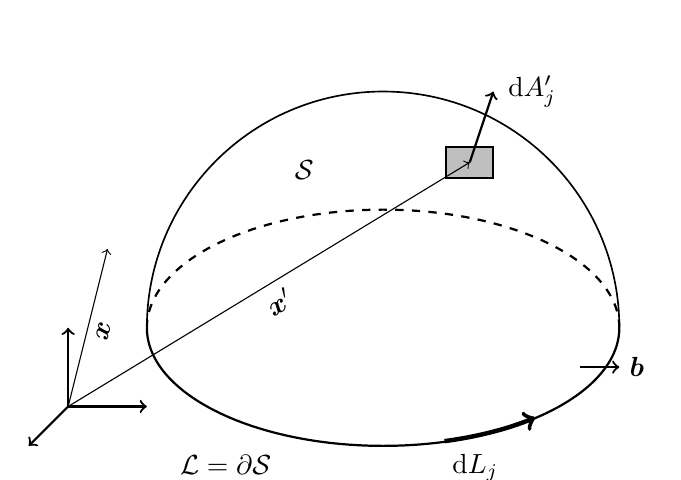
\begin{tikzpicture}
  \draw[semithick] (0,0) arc (0:180:3);
  \draw (-4,2) node {$\mathcal{S}$};
  \draw[dashed, thick] (0,0) arc [x radius=3, y radius=1.5, start angle=0, end angle=180];
  \draw[thick] (-6,0) arc [x radius=3, y radius=1.5, start angle=180, end angle=360];
  \draw[ultra thick, ->] (-2.22,-1.44) arc [x radius=3, y radius=1.5, start angle=285, end angle=310]
    node[below left, outer sep=10pt] {$\dL_j$};
  \filldraw[fill=gray!50!white, thick] (-2.2,2.3) rectangle (-1.6,1.9);
  \draw[thick, ->] (-1.9,2.1) -- (-1.6,3) node[right] {$\dA_j'$};
  \draw (-5,-1.5) node[below] {$\mathcal{L}=\partial\mathcal{S}$};
  \draw[->,thick] (-7,-1) -- (-7,-0); 
\draw[->,thick] (-7,-1) -- (-6,-1); 
\draw[->,thick] (-7,-1) -- (-7.5,-1.5); 
\draw[->] (-7,-1) --(-1.9,2.1)  node [sloped,below,text centered,midway]{$ \bm x'$}; 
\draw[->] (-7,-1) --(-6.5,1)  node [sloped,below,text centered,midway]{$ \bm x$}; 
\draw[->,thick] (-0.5,-0.5) --(-0,-0.5)  node [sloped,right,text centered]{$ \bm b$}; 
\end{tikzpicture}
\caption{The plastic distortion is concentrated on the surface $\mathcal{S}$, which is bounded by the dislocation line $\mathcal{L}=\partial\mathcal{S}$.}
\label{fig:dislocation_loop} 
\end{figure}
Let us know assume that the eigendistortion $\bm \beta^\star$ is only due to plastic deformation cause by dislocations, that is
\begin{align}
\bm \beta^\star=\bm \beta^P
\end{align}
The key equations of classical dislocation theory are now obtained by prescribing  the form of the eigendistortion tensor $\bm \beta^P$. For a dislocation extending over a surface $\mathcal{S}$,  the classical plastic eigendistortion tensor is taken in following form:
\begin{align}
\bPc_{kl}(\bm x)=-\int_\mathcal{S}\delta(\bm x-\bm x')b_k\dA_l'\, ,
\label{dislocation_distortion_classical}
\end{align}
where $\delta$ is the Dirac delta function, and $b_i$ is the displacement jump across $\mathcal{S}$, or Burgers vector. For a Volterra dislocation, as opposed to a Somigliana dislocation,  the Burgers vector is constant. In this case,  the  tensor $\alpha_{ij}=-\epsilon_{jkm}\bPc_{im,k}$ turns out to be concentrated on the dislocation line, that is the closed line $\mathcal{L}=\partial\mathcal{S}$ bounding the surface $\mathcal{S}$, and it is known as the \textit{dislocation density tensor}:
\begin{align}
\alpha_{ij}(\bm x)=\oint_{\mathcal{L}}\delta(\bm x-\bm x')b_i\dL_j'\, .
\label{dislocation_alpha_classical}
\end{align}
The rate of plastic distortion can be written in terms of the local dislocation velocity $w_k$ as
\begin{align}
\dot{\beta}^P_{ij}(\bm x)
=-\oint_{\mathcal{L}}\delta(\bm x-\bm x')b_i\epsilon_{jkm}w_k(\bm x')\dL_m'\,.
\label{plasticDistortionRateLoop}
\end{align}

Using the special forms (\ref{dislocation_distortion_classical}) and (\ref{dislocation_alpha_classical}) in the results obtained in the previous section we find all the key equations of classical dislocation theory in the anisotropic case. Letting $\bm R=\bm x-\bm x'$, these are:
\begin{subequations}
\begin{align}
u_i(\bm x)
&=-\frac{b_i\, \Omega(\bm
  x)}{4\pi}-\oint_{\mathcal{L}}\mathbb{C}_{mnpq}\epsilon_{jqr}b_pF_{jnim}(\bm
R)\dL_r' && \text{(anisotropic Burgers equation)}\\
\bEc_{ij}(\bm x)&=\oint_{\mathcal{L}}\mathbb{C}_{mnpq}\epsilon_{jqr}G_{im,n}(\bm R)b_p\dL_r' && \text{(Mura-Willis equation)}\\
\sigma_{ij}(\bm
x)&=\oint_{\mathcal{L}}\mathbb{C}_{ijkl}\mathbb{C}_{mnpq}\epsilon_{lqr}G_{km,n}(\bm
R)b_p\dL_r' && \text{(anisotropic Peach-Koehler stress equation)}\label{classicaCauchyStress}\\
W_{AB}&=\oint_{\mathcal{L}_A}\oint_{\mathcal{L}_B}\epsilon_{jkl}\mathbb{C}_{ilmn}\epsilon_{npq}\mathbb{C}_{rstp}F_{skmr}(\bm R)\, b^{A}_{t} b^{B}_{i} \dL^A_{q}\dL^B_{j}&&\text{(anisotropic Blin's formula) }\\
\mathcal{F}_k&=\oint_\mathcal{L}\epsilon_{kjm}\sigma_{ij}b_i\dL_m&&\text{(Peach-Koehler force)}
\end{align}
\label{class_aniso_all}
\end{subequations}
Note that, in the Burgers equation, we have introduced the solid angle  $\Omega(\bm x)$ subtended by the loop from the relationship  $\GP_{,j}*\bPc_{ij}=-{b_i\, \Omega}/{4\pi}$, which yields:
\begin{align}
\Omega(\bm x)=4\pi\int_\mathcal{S}\GP_{,j}\dA_j'=\int_\mathcal{S}\frac{R_j}{R^3}\dA_j'\, .
\end{align}

\begin{draftnote}The source notes stop before discussing the kernel of the preceding loop-field expressions. That missing derivation has not been reconstructed here.\end{draftnote}





%%%%%%%%%%%%%%%%%%%%%%
\subsection{Discrete dislocation loops in infinite isotropic media}
\begin{draftnote}The original isotropic specialization contains working equations but not a complete connecting derivation.\end{draftnote}
\begin{align}
\bm u=-\frac{\bm b\Omega}{4\pi}-\frac{1}{4\pi}\oint\left[\frac{\bm b\times\bm \xi}{R}+\frac{\lambda+\mu}{\lambda+2\mu}\left(\frac{\bm \xi\times\bm b}{R}-\frac{(\bm b\times\bm R)\cdot\bm \xi}{R^3}\bm R\right)\right]dl
\label{displcementIsotropicSolid}
\end{align}
where 
\begin{align}
\Omega=\int\frac{R_k\hat{n}_k}{R^3}dS=-\frac{1}{2}\int R_{,ppk}\hat{n}_kdS
\end{align}
When using the line integral expression of the solid angle (\ref{solidAngle2Line2}), eq.~(\ref{displcementIsotropicSolid}) becomes:
\begin{align}
\bm u&=\frac{1}{4\pi}\oint\left[\frac{(\bm s\times\bm R)\cdot\bm\xi}{R(R+\bm s\cdot\bm R)}\bm b+\frac{\bm \xi\times\bm b}{R}+\frac{1}{2(1-\nu)}\left(\frac{\bm b\times \bm \xi}{R}+\frac{(\bm b\times\bm R)\cdot\bm \xi}{R^3}\bm R\right)\right]dl\nonumber\\
&=\underbrace{\frac{1}{8\pi(1-\nu)}}_{c_4}\oint\frac{1}{R}\left[2\underbrace{(1-\nu)}_{c1}\frac{(\bm s\times\bm R)\cdot\bm\xi}{R+\bm s\cdot\bm R}\bm b+\underbrace{(1-2\nu)}_{c_3}\bm \xi\times\bm b+\frac{(\bm \xi\times\bm b)\cdot\bm R}{R^2}\bm R\right]dl
\label{displcementIsotropicLine}
\end{align}



%%%%%%%%%%%%%%%%%%%%%%
\subsubsection{Stress field}
\begin{equation}
\sigma_{ij}(\bm F)=\frac{\mu b_n}{8\pi}\int_\mathcal{S} \left[R_{,mpp}\left(\in_{jmn}\xi_i+\in_{imn}\xi_j\right)+\frac{2}{1-\nu}\in_{kmn}\left(R_{,ijm}-\delta_{ij}R_{,ppm}\right)\xi_k\right]dl^s
\end{equation}
where $\bm R=\bm F-\bm S$ is the vector connecting the source point to the field point and $\xi=\frac{d\bm S}{dl^s}$ s the unit tangent along the source dislocation. 

Substituting 
\begin{equation}
R_{,ijk}=-\frac{\delta_{ij}R_k+\delta_{jk}R_i+\delta_{ki}R_j}{R^3}+\frac{3R_iR_jR_k}{R^5} \ \ \ \ \ \ \    R_{,ipp}=-\frac{2R_i}{R^3}
\end{equation}

\begin{equation}
\sigma_{ij}(\bm F)=\frac{\mu b_n}{4\pi}\int_\mathcal{S} \left[-\frac{R_m}{R^3}\left(\in_{jmn}\xi_i+\in_{imn}\xi_j\right)+\frac{1}{1-\nu}\in_{kmn}\left(\frac{\delta_{ij}R_m-\delta_{jm}R_i-\delta_{mi}R_j}{R^3}+\frac{3R_iR_jR_m}{R^5}\right)\xi_k\right]dl^s
\end{equation}




or in dyadic form:

\begin{eqnarray}
\frac{d\bm \sigma}{dl}&=&\frac{\mu}{4\pi R^2}\left\{\hat{\bm\xi}\otimes(\bm b\times \hat{\bm R})+(\bm b\times \hat{\bm R})\otimes\hat{\bm\xi}\right.\nonumber\\
&+&\left.\frac{1}{1-\nu}\left[\hat{\bm R}\otimes(\hat{\bm\xi}\times\bm b)+(\hat{\bm\xi}\times\bm b)\otimes\hat{\bm R}
+ \left[(\hat{\bm R}\times\bm b)\cdot\hat{\bm\xi}\right]\left(\bm I + 3\hat{\bm R}\otimes\hat{\bm R} \right)\right]\right\}
%\frac{R_m}{R^3}\left(\in_{jmn}\xi_i+\in_{imn}\xi_j\right)+\frac{1}{1-\nu}\in_{kmn}\left(\frac{\delta_{ij}R_m-\delta_{jm}R_i-\delta_{mi}R_j}{R^3}+\frac{3R_iR_jR_m}{R^5}\right)\xi_k
\end{eqnarray}

more efficient to compute
\begin{eqnarray}
\frac{d\bm \sigma}{dl}&=&\frac{\mu}{4\pi (1-\nu)R^2}\left\{(1-\nu)\left[\hat{\bm\xi}\otimes(\bm b\times \hat{\bm R})+(\bm b\times \hat{\bm R})\otimes\hat{\bm\xi}\right]\right.\nonumber\\
&+&\left.\hat{\bm R}\otimes(\hat{\bm\xi}\times\bm b)+(\hat{\bm\xi}\times\bm b)\otimes\hat{\bm R}\right.\nonumber\\
&+&\left. \left[(\hat{\bm R}\times\bm b)\cdot\hat{\bm\xi}\right]\left(\bm I + 3\hat{\bm R}\otimes\hat{\bm R} \right)\right\}
%\frac{R_m}{R^3}\left(\in_{jmn}\xi_i+\in_{imn}\xi_j\right)+\frac{1}{1-\nu}\in_{kmn}\left(\frac{\delta_{ij}R_m-\delta_{jm}R_i-\delta_{mi}R_j}{R^3}+\frac{3R_iR_jR_m}{R^5}\right)\xi_k
\end{eqnarray}



or factoring the symmetric part

\begin{eqnarray}
\frac{d\bm \sigma}{dl}&=&\frac{\mu}{2\pi (1-\nu)R^2}\left\{(1-\nu)\hat{\bm\xi}\otimes(\bm b\times \hat{\bm R})
+\hat{\bm R}\otimes(\hat{\bm\xi}\times\bm b)
+\frac{1}{2}\left[(\hat{\bm R}\times\bm b)\cdot\hat{\bm\xi}\right]\left(\bm I + 3\hat{\bm R}\otimes\hat{\bm R} \right)\right\}_{sym}
%\frac{R_m}{R^3}\left(\in_{jmn}\xi_i+\in_{imn}\xi_j\right)+\frac{1}{1-\nu}\in_{kmn}\left(\frac{\delta_{ij}R_m-\delta_{jm}R_i-\delta_{mi}R_j}{R^3}+\frac{3R_iR_jR_m}{R^5}\right)\xi_k
\end{eqnarray}

where $\bm x_{\text{sym}}=\frac{1}{2}(\bm x+\bm x^T)$

%%%%%%%%%%%%%%%%%%%%%%%%%%%%%%%%%%%%%%%
\subsection{Line-integral representation of the solid angle subtended by a loop}

\begin{align}
 \bm u^0(\bm x)=-\frac{\bm b\Omega^0}{4\pi}-\frac{1}{8\pi(1-\nu)}\oint_\mathcal{L}&\frac{1}{R}\left\{\ 
 \left(1-2\nu\right) \bm b\times\hat{\bm \xi}'
+ \left[\hat{\bm R}\cdot\left(\bm b\times\hat{\bm \xi}' \right) \right]\hat{\bm R}  \right\}\dL'
\end{align}


\begin{align}
\bm\sigma^0(\bm x)=\frac{\mu}{4\pi(1-\nu)}\oint_{\mathcal{L}}&\frac{1}{R^2}\left\{
(1-\nu)\left[\hat{\bm\xi}'\otimes(\bm b\times\hat{\bm R})+(\bm b\times\hat{\bm R})\otimes\hat{\bm\xi}'\right] 
+\left[(\hat{\bm \xi}'\times\bm b)\otimes\hat{\bm R}+\hat{\bm R}\otimes(\hat{\bm \xi}'\times\bm b)\right] \right. \nonumber\\
&\left.+\hat{\bm R}\cdot(\bm b\times\hat{\bm\xi}')\left[3\hat{\bm R}\otimes\hat{\bm R}+\bm I \right]
\right\}\dL'
\end{align}


\subsubsection{Numerical implementation}

\begin{align}
 \mathbf{u}(\bm x)=-\frac{\mathbf{ b}\Omega(\mathbf x)}{4\pi}-\frac{1}{8\pi(1-\nu)}\oint_\mathcal{L}&\frac{1}{R}\left\{\ 
 \left(1-2\nu\right) \mathbf{ b}\times\hat{\mathbf{ \xi}}'
+ \left[\hat{\mathbf{ R}}\cdot\left(\mathbf{ b}\times\hat{\mathbf{ \xi}}' \right) \right]\hat{\mathbf{ R}}  \right\}\dL'
\end{align}
where $\mathbf{R}=\mathbf x-\mathbf x'$, and  $\Omega(\mathbf x)$ is the solid angle subtended by the surface $\mathcal{S}$:
\begin{align}
\Omega(\mathbf{x})=\int_\mathcal{S}\left(-\frac{1}{2}\partial_k\Delta R\right)\ dA'_k=\int_\mathcal{S} v_k(\mathbf R)\ dA'_k&&v_k(\mathbf y)=\frac{y_k}{y^3}
\end{align}
In order to transform the solid angle into a line integral, we need to introduce a fictitious vector field $v_k^f(\mathbf R)$ with the property $v^f_{k,k}=-v_{k,k}$. In this way we can find a vector potential $\Psi_m(\mathbf{R})$ for the divergence-less sum $v_k+v^f_k$. The vector potential satisfies both $v_k+v^f_k=\epsilon_{klm}\Psi_{m,l}$, and $\Psi_{k,k}=0$. Therefore, using Stokes theorem, we can write
\begin{align}
\Omega(\mathbf{x})&=\int_\mathcal{S} \left(\epsilon_{klm}\Psi_{m,l}-v^f_k\right)\ dA'_k=\int_\mathcal{S} \left(-\epsilon_{klm}\Psi_{m,l'}-v^f_k\right)\ dA'_k\nonumber\\
&=-\oint_\mathcal{L}\Psi_m\ dL'_m-\int_\mathcal{S} v^f_k\ dA'_k=-\oint_\mathcal{L}\Psi_i\ dL'_i-\Omega^f
\end{align}
Note that there is an error in Po-Lazar 2014, where the first term in the last equation has the wrong sign.
We now need to find the vector potential $\Psi_i$ and the fictitious vector field $v_i^f$. To do this we consider the auxiliary curve (Dirac string) $\mathcal{D}$, starting from $\mathbf x$ and ending at a point at infinity. Using the Dirac string, the fictitious vector can be found as
\begin{align}
v^f_{k}(\mathbf{R})=\int_\mathcal{D}v_{m,m}(\mathbf{R}+\mathbf{s})ds_k
=\int_\mathcal{D}\left(-\frac{1}{2}\Delta\Delta |\mathbf{x}+\mathbf{s}|\right)ds_k
=4\pi\int_\mathcal{D}\delta(\mathbf{R}+\mathbf{s})ds_k
\end{align}
The aforementioned property of $\mathbf v^f$ can be verified as follows:
\begin{align}
v^f_{k,k}(\mathbf{R})
&=\frac{\partial}{\partial x_k}\int_\mathcal{D}v_{m,m}(\mathbf{R}+\mathbf{s})ds_k
=\int_\mathcal{D}\frac{\partial}{\partial x_k}v_{m,m}(\mathbf{R}+\mathbf{s})ds_k\nonumber\\
&=\int_\mathcal{D}\frac{\partial}{\partial s_k}v_{m,m}(\mathbf{R}+\mathbf{s})ds_k
=\left[v_{m,m}(\mathbf{R}+\mathbf{s})\right]_\mathbf{0}^\infty=-v_{m,m}(\mathbf{R})
\end{align}

Knowing the fictitious vector, the vector potential can be found observing that  
\begin{align}
-\Delta \Psi_i=\epsilon_{ijk}(v_k+v^f_k)_{,j}=\epsilon_{ijk}v^f_{k,j}=-\epsilon_{ijk}\partial_j\int_\mathcal{D}\frac{1}{2}\Delta\Delta |\mathbf{R}+\mathbf{s}|ds_k
\end{align}
Therefore
\begin{align}
\Psi_i(\mathbf R)=\epsilon_{ijk}\int_\mathcal{D}\frac{1}{2}\partial_j\Delta |\mathbf{R}+\mathbf{s}|ds_k=-\epsilon_{ijk}\int_\mathcal{D}\frac{R_j+s_j}{|\mathbf{R}+\mathbf{s}|^3}ds_k
\end{align}
Choosing the Dirac string to be a straight line with unit direction $\hat{\mathbf{s}}$, the expression above becomes:
\begin{align}
\Psi_i(\mathbf R)&
=-\epsilon_{ijk}\int_0^\infty\frac{R_j+\alpha \hat{s}_j}{|\mathbf{R}+\alpha\hat{\mathbf{s}}|^3}\hat{s}_k\ d\alpha
=-\epsilon_{ijk}R_j\hat{s}_k\int_0^\infty\frac{1}{|\mathbf{R}+\alpha\hat{\mathbf{s}}|^3}\ d\alpha\nonumber\\
&=-\epsilon_{ijk}R_j\hat{s}_k\left[\frac{\alpha+\mathbf{R}\cdot\hat{\mathbf{s}}}{\left(R^2-(\mathbf{R}\cdot\hat{\mathbf{s}})^2\right)|\mathbf R+\alpha\hat{\mathbf s}|}\right]_0^\infty\nonumber\\
&=-\epsilon_{ijk}R_j\hat{s}_k\left[\frac{1}{R^2-(\mathbf{R}\cdot\hat{\mathbf{s}})^2}
-\frac{\mathbf{R}\cdot\hat{\mathbf{s}}}{\left(R^2-(\mathbf{R}\cdot\hat{\mathbf{s}})^2\right)R}\right]\nonumber\\
&=-\epsilon_{ijk}R_j\hat{s}_k
\frac{R-\mathbf{R}\cdot\hat{\mathbf{s}}}{\left(R^2-(\mathbf{R}\cdot\hat{\mathbf{s}})^2\right)R}
=-\frac{\epsilon_{ijk}R_j\hat{s}_k}{R\left(R+\mathbf{R}\cdot\hat{\mathbf{s}}\right)}
\end{align}
In vector form this reads
\begin{align}
\mathbf{\Psi}(\mathbf{x})=-\frac{\mathbf{R}\times\hat{\mathbf{s}}}{R\left(R+\mathbf{R}\cdot\hat{\mathbf{s}}\right)}
\end{align}

Finally, the Burgers equation becomes
\begin{align}
 \mathbf{u}(\mathbf x)
 &=-\frac{\mathbf{ b}}{4\pi}\left(-\oint_\mathcal{L}\Psi_i(\mathbf{R})\ dL'_i-\Omega^f\right)-\frac{1}{8\pi(1-\nu)}\oint_\mathcal{L}\frac{1}{R}\left\{\ 
 \left(1-2\nu\right) \mathbf{ b}\times\hat{\mathbf{ \xi}}'
+ \left[\hat{\mathbf{ R}}\cdot\left(\mathbf{ b}\times\hat{\mathbf{ \xi}}' \right) \right]\hat{\mathbf{ R}}  \right\}\dL'\nonumber\\
&=\frac{\mathbf{ b}\Omega^f}{4\pi}
-\frac{\mathbf{ b}}{4\pi}\oint_\mathcal{L}\frac{(\mathbf{R}\times\hat{\mathbf{s}})\cdot\hat{\mathbf{\xi}}'}{R\left(R+\mathbf{R}\cdot\hat{\mathbf{s}}\right)}\ dL'
-\frac{1}{8\pi(1-\nu)}\oint_\mathcal{L}\frac{1}{R}\left\{\ 
 \left(1-2\nu\right) \mathbf{ b}\times\hat{\mathbf{ \xi}}'
+ \left[\hat{\mathbf{ R}}\cdot\left(\mathbf{ b}\times\hat{\mathbf{ \xi}}' \right) \right]\hat{\mathbf{ R}}  \right\}\dL'\nonumber\\
&=\mathbf{b}^f(\mathbf x)
-\frac{1}{8\pi(1-\nu)}\oint_\mathcal{L}   
\frac{1}{R}\left\{\ \frac{2(1-\nu)(\hat{\mathbf{R}}\times\hat{\mathbf{s}})\cdot\hat{\mathbf{\xi}}'}{1+\hat{\mathbf{R}}\cdot\hat{\mathbf{s}}}\mathbf{ b}
+ \left(1-2\nu\right) \mathbf{ b}\times\hat{\mathbf{ \xi}}'
+ \left[\hat{\mathbf{ R}}\cdot\left(\mathbf{ b}\times\hat{\mathbf{ \xi}}' \right) \right]\hat{\mathbf{ R}}  \right\}\dL'\nonumber\\
&=\mathbf{b}^f(\mathbf x)
+\frac{1}{8\pi(1-\nu)}\oint_\mathcal{L}   
\frac{1}{R}\left\{\ \frac{2(1-\nu)(\hat{\mathbf{s}}\times\hat{\mathbf{R}})\cdot\hat{\mathbf{\xi}}'}{1+\hat{\mathbf{R}}\cdot\hat{\mathbf{s}}}\mathbf{ b}
+ \left(1-2\nu\right) \hat{\mathbf{ \xi}}'\times \mathbf{ b}
+ \left[\hat{\mathbf{ R}}\cdot\left(\hat{\mathbf{ \xi}}'\times\mathbf{ b} \right) \right]\hat{\mathbf{ R}}  \right\}\dL'\nonumber\\
\end{align}

Notice that
\begin{align}
\mathbf{b}^f(\mathbf x)
&=\frac{\mathbf{ b}\Omega^f}{4\pi}
=\frac{\mathbf{ b}}{4\pi}\int_\mathcal{S} v^f_k(\mathbf{R})\ dA'_k
=\frac{\mathbf{ b}}{4\pi}\int_\mathcal{S} 4\pi\int_\mathcal{D}\delta(\mathbf{R}+\mathbf{s})ds_k\ dA'_k\nonumber\\
&=\begin{cases}
+\mathbf{b}&\mbox{if the Dirac string crosses the slip surface positively}\\
-\mathbf{b}&\mbox{if the Dirac string crosses the slip surface negatively}\\
\mathbf{0}&\mbox{if the Dirac string does not cross the slip surface }
\end{cases}
\end{align}

%%%%%%%%%%%%%%%%%%%%%%%%%
\subsection{Multipole expansion}

\subsubsection{Stress field}
\begin{align}
\sigma_{ij}=\oint_\mathcal{L}S_{ijkl}R(\mathbf x-\mathbf x')b'_k\xi'_l\ dL'
\end{align}
Now let $\mathbf{x'}=\mathbf{x}^c-\tilde{\mathbf{x}}$, then
\begin{align}
\sigma_{ij}=\oint_\mathcal{L}S_{ijkl}R(\mathbf x-\mathbf x^c+\tilde{\mathbf{x}})b'_k\xi'_l\ dL'
\end{align}
Now assume 
\begin{align}
|\tilde{\mathbf{x}}|\ll |\mathbf x-\mathbf x^c|
\end{align}
then, expanding $R$ for $\tilde{\mathbf{x}}\rightarrow0$ yields
\begin{align}
R(\mathbf x-\mathbf x^c+\tilde{\mathbf{x}})\approx R(\mathbf x-\mathbf x^c)+\partial_pR(\mathbf x-\mathbf x^c)\tilde{x}_p+\ldots
\end{align}
and
\begin{align}
\sigma_{ij}=S_{ijkl}R(\mathbf x-\mathbf x^c)\oint_\mathcal{L}b'_k\xi'_l\ dL'+S_{ijkl}\partial_pR(\mathbf x-\mathbf x^c)\oint_\mathcal{L}\tilde{x}_pb'_k\xi'_l+\ldots
\end{align}

First order expansion:
\begin{align}
\bm\sigma^0(\bm x)=\frac{\mu}{4\pi(1-\nu)R^2}&\left\{
(1-\nu)\left[\hat{\bm\xi}'\otimes(\bm b\times\hat{\bm R})+(\bm b\times\hat{\bm R})\otimes\hat{\bm\xi}'\right] 
+\left[(\hat{\bm \xi}'\times\bm b)\otimes\hat{\bm R}+\hat{\bm R}\otimes(\hat{\bm \xi}'\times\bm b)\right] \right. \nonumber\\
&\left.+\hat{\bm R}\cdot(\bm b\times\hat{\bm\xi}')\left[3\hat{\bm R}\otimes\hat{\bm R}+\bm I \right]
\right\}
\end{align}
Letting
\begin{align}
(\bm b\times\hat{\bm R})\otimes\hat{\bm\xi})_{ij}=\epsilon_{ikm}b_kR_m\xi_j=\epsilon_{ikm}R_m\alpha_{kj}=\mathbf{S}\cdot\mathbf{\alpha}
\end{align}
\begin{align}
\mathbf{S}=\left[\begin{array}{ccc}
0&R_3&-R_2\\
-R_3&0&R_1\\
R_2&-R_1&0
\end{array}\right]
\end{align}
\begin{align}
\bm b\times\hat{\bm \xi}'=\epsilon_{ikm}b_k\xi_m=a_i
\end{align}
\begin{align}
\mathbf{a}=\left[\begin{array}{c}
\alpha_{23}-\alpha_{32}\\
\alpha_{31}-\alpha_{13}\\
\alpha_{12}-\alpha_{21}
\end{array}\right]
\end{align}
we obtain
\begin{align}
\bm\sigma^0(\bm x)=\frac{\mu}{4\pi(1-\nu)R^2}&\left\{
(1-\nu)\left[(\mathbf{S}\cdot\mathbf{\alpha})^T+\mathbf{S}\cdot\mathbf{\alpha}\right] 
-\left[\mathbf{a}\otimes\hat{\bm R}+\hat{\bm R}\otimes\mathbf{a}\right] \right. \nonumber\\
&\left.+(\hat{\bm R}\cdot\bm a)\left[3\hat{\bm R}\otimes\hat{\bm R}+\bm I \right]
\right\}
\end{align}

\subsubsection{Displacement field}
\begin{align}
 \mathbf{u}(\mathbf x)
&=\mathbf{b}^f(\mathbf x)
+\frac{1}{8\pi(1-\nu)}  \frac{1}{R}
\left\{\ \bm\alpha\cdot\frac{2(1-\nu)(\hat{\mathbf{s}}\times\hat{\mathbf{R}})}{1+\hat{\mathbf{R}}\cdot\hat{\mathbf{s}}}
- \left(1-2\nu\right) \bm a
- \left(\hat{\mathbf{ R}}\cdot\bm a \right)\hat{\mathbf{ R}}  \right\}
\end{align}

\subsubsection{Interaction Energy}

\begin{align}
E_I=-\frac{\mu}{4\pi(1-\nu)}\oint_{\mathcal{L}_{2}}\oint_{\mathcal{L}_{1}}&\frac{1}{R}\left\{\left[(1-\nu)\left(\bm b_{1}\cdot\hat{\bm \xi}_1\right)\left(\bm b_{2}\cdot\hat{\bm \xi}_{2}\right)
+2\nu\left( \bm b_1\cdot\hat{\bm \xi}_2\right)\left(\bm b_2\cdot\hat{\bm \xi}_1\right)
-2\left(\bm b_1\cdot{\bm b}_2\right)\left( \hat{\bm\xi}_1\cdot\hat{\bm \xi}_2\right)
\right]\right.\nonumber\\
&\left.+\left( \hat{\bm\xi}_1\cdot\hat{\bm \xi}_2\right) \left[\left(\bm b_1\cdot\bm b_2\right)-\left(\bm b_1\cdot\hat{\bm R}\right)\left(\bm b_2\cdot\hat{\bm R}\right)\right]\right\} dL_{1} dL_{2}
\label{interaction_energy_loop_vector_expanded}
\end{align}

\begin{align}
E_I=-\frac{\mu}{4\pi(1-\nu)}\oint_{\mathcal{L}_{2}}\oint_{\mathcal{L}_{1}}&\frac{1}{R}\left\{(1-\nu)\left(\bm b_{1}\cdot\hat{\bm \xi}_1\right)\left(\bm b_{2}\cdot\hat{\bm \xi}_{2}\right)
+2\nu\left( \bm b_1\cdot\hat{\bm \xi}_2\right)\left(\bm b_2\cdot\hat{\bm \xi}_1\right)
-\left(\bm b_1\cdot{\bm b}_2\right)\left( \hat{\bm\xi}_1\cdot\hat{\bm \xi}_2\right)
\right.\nonumber\\
&\left. -\left( \hat{\bm\xi}_1\cdot\hat{\bm \xi}_2\right)\left(\bm b_1\cdot\hat{\bm R}\right)\left(\bm b_2\cdot\hat{\bm R}\right)\right\} dL_{1} dL_{2}
\label{interaction_energy_loop_vector}
\end{align}










%%%%%%%%%%%%%%%%%%%%%%%%%
\subsection{Plastic strain rate}

For conservative motion (glide) $\bm v\cdot\hat{\bm n}=0$, therefore, from (\ref{STT2L}):
\begin{align}
\dot\beta^p_{ij}(\bm x)=-b_i\int_{\bm A}^{\bm B}\delta(\bm x-\bm x')\epsilon_{jkm}v_kdl'_m
\end{align}


%%%%%%%%%%%%%%%%%%%%%%%%%
%%%%%%%%%%%%%%%%%%%%%%%%%





%%%%%%%%%%%%%%%%%%%%%%%%%
%%%%%%%%%%%%%%%%%%%%%%%%%






%%%%%%%%%%%%%%%%%%%%%%%%%%%%%%%%%%%%%%%%%%
\subsection{Discrete dislocations in finite media}

From a numerical viewpoint, it is interesting to ask; what is the distribution of $\beta^P_{ij}$ outside $\mathcal{B}$ in (\ref{BVPinfinite})? We shall call this quantity $\beta^{P*}_{ij}$. In fact, although the solution to the problems (\ref{BVPinfinite}) and (\ref{BVPcorrection}) depend individually on $\beta^{P*}_{ij}$, it is easy to see that the total solution is independent of  $\beta^{P*}_{ij}$. Therefore $\beta^{P*}_{ij}$ can be chosen arbitrarily\footnote{We observe that the arbitrariness of $\beta^{P*}_{ij}$ implies that also its bounding curve (or virtual dislocation line) is arbitrary, in agreement with the ``mirror image construction" of \cite{Weygand:2002tq}  and the ``independence of the total stress on the choice of virtual segments'' mentioned in \cite{Weinberger:2009fk}.}.  The arbitrariness of $\beta^{P*}_{ij}$ can be exploited in the numerical implementation. To see how, we can cast  (\ref{BVPcorrection}) in its   corresponding Galerkin weak form
\begin{align}
\int_\mathcal{B}c_{ijkl}u^c_{k,l}\tilde{u}_{i,j}d\mathcal{V}=\int_{\partial_N\mathcal{B}}\left(p_i- \sigma^\infty_{ij}\hat{n}_j\right)\tilde{u}_id\mathcal{A}
\label{BVPcorrectionWeak}
\end{align} 
and notice that the RHS involves a surface integral  of the stress field  $\sigma^\infty_{ij}$ induced by the dislocation network. When a dislocation segment reaches the domain boundary, the numerical evaluation of this integral becomes challenging. This numerical difficulty can be  overcome using the external-loop construction in Fig.~\ref{BVPStrategy}. In fact, because $\beta^{P*}_{ij}$ is arbitrary, it is possible to add an external loop with the same Burgers vector of the boundary segment and opposite line direction, constructed so that one side of the loop overlaps with the boundary segment, and the opposite side is pushed to infinity along the direction of the boundary normal vector. In this way, because the contributions of the overlapping segments cancel out, the line integral involved in the calculation of $\sigma^{\infty}_{ij}$ can be limited to the portion of the dislocation configuration strictly inside the domain, and the virtual straight dislocation lines extending from the domain boundary to infinity. Notice that this construction unambiguously defines $\beta^{P*}_{ij}$ and the surface over which it extends, a fundamental requirement for the calculation of $u^\infty_i$ needed to satisfy displacement boundary conditions in the BVP (\ref{BVPcorrection}).

%%%%%%%%%%%%%%%%%%%%%%%%%

\begin{figure}[htbp]\centering
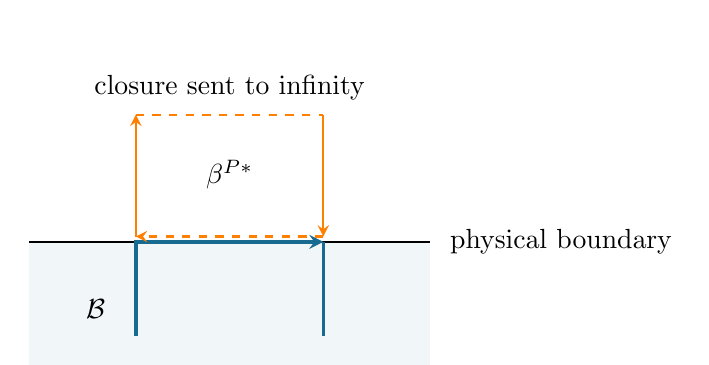
\begin{tikzpicture}[scale=0.85,>=stealth]
\fill[manualblue!6] (-3,-2) rectangle (3,0);
\draw[thick] (-3,0)--(3,0);
\node at (-2,-1) {$\mathcal B$};
\draw[very thick,manualblue,->] (-1.4,-1.4)--(-1.4,0)--(1.4,0);
\draw[very thick,manualblue] (1.4,0)--(1.4,-1.4);
\draw[thick,orange,dashed,->] (1.4,0.08)--(-1.4,0.08);
\draw[thick,orange,->] (-1.4,0.08)--(-1.4,1.9);
\draw[thick,orange,<-] (1.4,0.08)--(1.4,1.9);
\draw[thick,orange,dashed] (-1.4,1.9)--(1.4,1.9);
\node at (0,2.3) {closure sent to infinity};
\node at (0,1) {$\beta^{P*}$};
\node[anchor=west] at (3.15,0) {physical boundary};
\end{tikzpicture}
\caption{Schematic external-loop construction. Oppositely oriented overlapping boundary segments cancel; the external closure is taken to infinity. The drawing shows connectivity, not a finite computational truncation prescription.}
\label{BVPStrategy}
\end{figure}

\subsection{Force vector of a triangular element due to a straight segment}
We would like to compute the force vector of a triangular boundary element due to a straight segment. The weak form involved in the FEM problem is
\begin{align}
\int_\mathcal{T}\tilde u_i t_i \text{d}A=\sum_n \tilde u^n_i\int_\mathcal{T}N^n \sigma_{ij}\hat{n}_j \text{d}A
\end{align}
where $N^n$ is the shape function of the $n$-th node of the triangle, and $\tilde u^n_i$ its test displacement. 
The stress field generated by the dislocaiton loops is
\begin{align}
\sigma_{ij}(\bm x)=\tilde{S}_{ijl}\left[q_l(\bm x)\right]
\end{align}
where 
\begin{align}
q_l(\bm x)=\oint_\mathcal{L}R_a(\bm x-\bm x')\ d\ell'_l
\end{align}
and $\tilde{S}$ is the the third-order dislocation stress differential operator, which is defined as
\begin{align}
\tilde{S}_{ijl}[\cdot]=\frac{\mu b_k}{8\pi}\left[\left(\delta_{il}\epsilon_{jmk}+\delta_{jl}\epsilon_{imk}\right)\partial_m\Delta+\frac{2}{1-\nu}\epsilon_{klm}\left(\partial_{i}\partial_j\partial_m-\delta_{ij}\partial_m\Delta\right)\right]
\end{align}
\begin{draftnote}The following operator manipulation was highlighted as working material in the original notes. It is retained for review, not promoted to a verified implementation formula.\end{draftnote}
{
Note that this operator can be rewritten as 
\begin{align}
\tilde{S}_{ijl}[\cdot]=\partial_m\hat{S}_{ijlm}[\cdot]
\end{align}
where the auxiliary second-order differential operator $\hat{S}_{ijlm}[\cdot]$ is
\begin{align}
\tilde{S}_{ijlm}[\cdot]=\frac{\mu b_k}{8\pi}\left[\left(\delta_{il}\epsilon_{jmk}+\delta_{jl}\epsilon_{imk}\right)\Delta+\frac{2}{1-\nu}\epsilon_{klm}\left(\partial_{i}\partial_j-\delta_{ij}\Delta\right)\right]
\end{align}
Let us focus on the integral
\begin{align}
F^{(n)}_{i}&=\int_\mathcal{T}N^{(n)} \sigma_{ij}\text{d}A_j
=\int_\mathcal{T}N^n \partial_m \hat{S}_{ijlm}\left[q_l(\bm x)\right]\, \text{d}A_j\nonumber\\
&=\int_\mathcal{T}\partial_m\left\{N^n  \hat{S}_{ijlm}\left[q_l(\bm x)\right]\, \right\}\text{d}A_j
-\int_\mathcal{T}N^n_{,m}  \hat{S}_{ijlm}\left[q_l(\bm x)\right]\, \text{d}A_j
\label{FEMforceVectorDD1}
\end{align}
We now apply Stokes theorem \eqref{KelvinStokesCorollary} to the first term of \eqref{FEMforceVectorDD1} to find
\begin{align}
F^{(n)}_{i}
&=
\oint_{\partial \mathcal{T}}\epsilon_{kjm}N^{(n)}\hat{S}_{ijlm}\left[q_l(\bm x)\right]\, \text{d}\ell_k
+\int_\mathcal{T}\partial_j\left\{N^n  \hat{S}_{ijlm}\left[q_l(\bm x)\right]\, \right\}\, \text{d}A_m
-\int_\mathcal{T}N^n_{,m}  \hat{S}_{ijlm}\left[q_l(\bm x)\right]\, \text{d}A_j\nonumber\\
&=
\oint_{\partial \mathcal{T}}\epsilon_{kjm}N^{(n)}\hat{S}_{ijlm}\left[q_l(\bm x)\right]\, \text{d}\ell_k
+\int_\mathcal{T} N^n  \partial_j\hat{S}_{ijlm}\left[q_l(\bm x)\right]\, \text{d}A_m\nonumber\\
&+\int_\mathcal{T}N^n_{,j}  \hat{S}_{ijlm}\left[q_l(\bm x)\right]\, \, \text{d}A_m
-\int_\mathcal{T}N^n_{,m}  \hat{S}_{ijlm}\left[q_l(\bm x)\right]\, \text{d}A_j\nonumber\\
\label{FEMforceVectorDD2}
\end{align}
Note that in the expression above, the only third-order differential operator is $\partial_j\hat{S}_{ijlm}$. However a closer inspection reveals that
\begin{align}
\partial_j\hat{S}_{ijlm}\left[q_l(\bm x)\right]
&=\frac{\mu b_k}{8\pi}\left[\left(\delta_{il}\epsilon_{jmk}+\delta_{jl}\epsilon_{imk}\right)\partial_j\Delta+\frac{2}{1-\nu}\epsilon_{klm}\cancel{\left(\partial_{i}\partial_j\partial_j-\delta_{ij}\partial_j\Delta\right)}\right]\left[q_l(\bm x)\right]\nonumber\\
%&=\frac{\mu b_k}{8\pi}\left(\epsilon_{jmk}\Delta\partial_j \left[q_i(\bm x)\right]+\epsilon_{imk}\Delta\partial_l \left[q_l(\bm x)\right]\right)\nonumber
&=\frac{\mu b_k}{8\pi}\left(\epsilon_{jmk}\Delta\partial_j \left[q_i(\bm x)\right]+\epsilon_{imk}\Delta \left[\oint_\mathcal{L} \frac{\partial}{\partial x_l} R_a(\bm x-\bm x')\ d\ell'_l\right]\right)\nonumber\\
&=\frac{\mu b_k}{8\pi}\left(\epsilon_{jmk}\Delta\partial_j \left[q_i(\bm x)\right]-\epsilon_{imk}\Delta \left[\cancel{\oint_\mathcal{L} \frac{\partial}{\partial x'_l} R_a(\bm x-\bm x')\ d\ell'_l}\right]\right)\nonumber
\end{align}
The first term is zero if the Burgers vector is aligned with the surface normal (not very useful).
Moreover
\begin{align}
\epsilon_{kjm}\tilde{S}_{ijlm}
&=\frac{\mu b_p}{8\pi}\left[\left(\delta_{il}\epsilon_{kjm}\epsilon_{jmp}+\delta_{jl}\epsilon_{mkj}\epsilon_{mpi}\right)\Delta+\frac{2}{1-\nu}\epsilon_{mkj}\epsilon_{mpl}\left(\partial_{i}\partial_j-\delta_{ij}\Delta\right)\right]\nonumber\\
&=\frac{\mu b_p}{8\pi}\left[\left(\delta_{il}2\delta_{kp}+\delta_{jl}\left(\delta_{kp}\delta_{ij}-\delta_{ik}\delta_{jp}\right)\right)\Delta+\frac{2}{1-\nu}\left(\delta_{kp}\delta_{jl}-\delta_{kl}\delta_{jp}\right)\left(\partial_{i}\partial_j-\delta_{ij}\Delta\right)\right]\nonumber\\
&=\frac{\mu b_p}{8\pi}\left[\left(2\delta_{il}\delta_{kp}+\delta_{kp}\delta_{il}-\delta_{ik}\delta_{lp}\right)\Delta+\frac{2}{1-\nu}\left(\delta_{kp}\delta_{jl}-\delta_{kl}\delta_{jp}\right)\left(\partial_{i}\partial_j-\delta_{ij}\Delta\right)\right]
\end{align}
}
Moreover
\begin{align}
\epsilon_{kjm}\tilde{S}_{ijlm}[\cdot]
&=\frac{\mu b_p}{8\pi}\left[\left(\delta_{il}\epsilon_{kjm}\epsilon_{jmp}+\delta_{jl}\epsilon_{kjm}\epsilon_{imp}\right)\Delta+\frac{2}{1-\nu}\epsilon_{kjm}\epsilon_{plm}\left(\partial_{i}\partial_j-\delta_{ij}\Delta\right)\right]\nonumber\\
&=\frac{\mu b_p}{8\pi}\left[\left(2\delta_{il}\delta_{pk}+\delta_{jl}(\delta_{kp}\delta_{ji}-\delta_{ki}\delta_{jp})\right)\Delta+\frac{2}{1-\nu}(\delta_{kp}\delta_{jl}-\delta_{kl}\delta_{jp})\left(\partial_{i}\partial_j-\delta_{ij}\Delta\right)\right]\nonumber\\
&=\frac{\mu b_p}{8\pi}\left[\left(2\delta_{il}\delta_{pk}+\delta_{kp}\delta_{li}-\delta_{ki}\delta_{lp}\right)\Delta+\frac{2}{1-\nu}(\delta_{kp}\delta_{jl}-\delta_{kl}\delta_{jp})\left(\partial_{i}\partial_j-\delta_{ij}\Delta\right)\right]\nonumber\\
\end{align}


%For a straight segment starting at $\bm A$ and ending at $\bm B$
%\begin{align}
%\bm x'(u)=\bm A(1-u)+\bm Bu=\bm A+(\bm B-\bm A)u\hspace{1cm} u\in[0,1]
%\end{align}


%%%%%%%%%%%%%%%%%%%%%%%%%%%%%%%%%%%%%%%%%%
\subsection{Discrete dislocations in periodic media}
The translation lattice is described in Section~\ref{sec:periodicity}; finite-image controls and periodic glide-plane geometry are described in Section~\ref{sec:dddPeriodicity}. The original notes supplied only this heading; a complete periodic elastic-sum derivation remains to be written.
\chapter{DDD: regularization of singular fields}
\begin{draftnote}
These finite-core expressions were previously outside the compiled manual. They are retained as working theory; the index notation and equivalence of the component and dyadic forms still require a dedicated mathematical review. The inherited Levi--Civita notation is standardized to $\epsilon_{ijk}$.
\end{draftnote}
The regularized distance is $R_a=\sqrt{\bm R\cdot\bm R+a^2}$. The plot below illustrates the smoothing of this distance.
\section{Stress kernel}
\begin{equation}
\sigma^\text{ns}_{ij}(\bm F)=\frac{\mu b_n}{8\pi}\int_\mathcal{S} \left[R_{a,mpp}\left(\epsilon_{jmn}\xi_i+\epsilon_{imn}\xi_j\right)+\frac{2}{1-\nu}\epsilon_{kmn}\left(R_{a,ijm}-\delta_{ij}R_{a,ppm}\right)\xi_k\right]dl^s
\end{equation}
where $\bm R=\bm F-\bm S$ is the vector connecting the source point to the field point and $\xi=\frac{d\bm S}{dl^s}$ s the unit tangent along the source dislocation. 

Substituting 
\begin{equation}
R_{,ijk}=-\frac{\delta_{ij}R_k+\delta_{jk}R_i+\delta_{ki}R_j}{R_a^3}+\frac{3R_iR_jR_k}{R_a^5} \ \ \ \ \ \ \    R_{a,ipp}=-\left(2+\frac{3a^2}{R_a^2}\right)\frac{R_i}{R_a^3}
\end{equation}
we find
\begin{equation}
\begin{split}
\sigma_{ij}(\bm F)=\frac{\mu b_n}{4\pi}\int_\mathcal{S} &\left[-\left(1+\frac{3a^2}{2R_a^2}\right)\frac{R_m}{R_a^3}\left(\epsilon_{jmn}\xi_i+\epsilon_{imn}\xi_j\right)\right.
\\ &\left.+\frac{1}{1-\nu}\epsilon_{kmn}\left(\frac{\delta_{ij}\left(1+\frac{3a^2}{R_a^2}\right)R_m-\delta_{jm}R_i-\delta_{mi}R_j}{R_a^3}+\frac{3R_iR_jR_m}{R_a^5}\right)\xi_k\right]dl^s
\end{split}
\end{equation}
In dyadic form
\begin{align}
\frac{d\bm \sigma}{d L}=\frac{\mu }{4\pi (1-\nu)R_a^2}&\left\{(1-\nu)\left(1+\frac{3a^2}{2R_a^2}\right)\left(\hat{\bm\xi}\otimes (\bm b\times \tilde{\bm R})+ (\bm b\times \tilde{\bm R})\otimes\hat{\bm\xi}\right)\right.\nonumber\\
&\left.+\left(\tilde{\bm R}\otimes(\hat{\bm\xi}\times\bm b)+(\hat{\bm\xi}\times\bm b)\otimes \tilde{\bm R}\right)\right\}\nonumber\\
%
&\left.+[(\tilde{\bm R}\times\bm b)\cdot\hat{\bm \xi}]\left[\left(1+\frac{3a^2}{R_a^2}\right)\bm I+3\tilde{\bm R}\otimes \tilde {\bm R}\right]\right\}
\end{align}
where $\tilde{\bm R}=\bm R/R_a$\manualfigure{regularized_distance}{0.8}{Analytical distance kernel $R_a=\sqrt{x^2+a^2}$ for two core radii. This illustrates the smoothing operation, not the full dislocation stress or a simulated core structure.}


\chapter{DDD: fields of piecewise-straight loops}



%%%%%%%%%%%%%%%%%%%%%%%%%
\section{Straight segments}
For a straight segment starting at $\bm A$ and ending at $\bm B$, it is useful to preliminary compute the function
\begin{align}
q(\bm x)=\int_{\bm A}^{\bm B}R_a\ d\ell'
\end{align}
where $R_a=\sqrt{\bm R\cdot\bm R+a^2}$, $\bm R=\bm x-\bm x'$. Integration is performed on the primed variable along the segment $\bm A\bm B$. This can be parametrized as a function of a scalar variable $u$ as
\begin{align}
\bm x'(u)=\bm A(1-u)+\bm Bu=\bm A+(\bm B-\bm A)u\hspace{1cm} u\in[0,1]
\end{align}
Therefore
\begin{align}
q(\bm x)&=L\int_0^1\sqrt{[(\bm A-\bm x)+(\bm B-\bm A)u]^2+a^2}\ du\nonumber\\
&=L\int_0^1\sqrt{(\bm B-\bm A)^2u^2+2(\bm A-\bm x)\cdot(\bm B-\bm A)u+(\bm A-\bm x)^2+a^2}\ du
\end{align}
Now
\begin{align}
\int\sqrt{du^2+bu+c}\ du=\left(\frac{b}{4d}+\frac{u}{2}\right)\sqrt{du^2+bu+c}+\frac{4dc-b^2}{8d^\frac{3}{2}}\ln\left(\frac{2du+b}{\sqrt{d}}+2\sqrt{du^2+bu+c}\right)
\end{align}
So
\begin{align}
\int_0^1\sqrt{du^2+bu+c}\ du=&\frac{2d+b}{4d}\sqrt{d+b+c}-\frac{b}{4d}\sqrt{c}+\frac{4dc-b^2}{8d^\frac{3}{2}}\ln\left(\frac{\frac{2d+b}{\sqrt{d}}+2\sqrt{d+b+c}}{\frac{b}{\sqrt{d}}+2\sqrt{c}}\right)
\end{align}

Note that in our case
\begin{align}
d&=(\bm B-\bm A)^2=L^2\\
b&=2(\bm A-\bm x)\cdot(\bm B-\bm A)=2L(\bm A-\bm x)\cdot\hat{\bm\xi}\\
c&=(\bm A-\bm x)^2+a^2\\
d+b+c&=(\bm B-\bm x)^2+a^2\\
2d+b&=2(\bm B-\bm x)\cdot(\bm B-\bm A)=2L(\bm B-\bm x)\cdot{\hat{\bm \xi}}\\
4dc-b^2&=4(\bm B-\bm A)^2(\bm A-\bm x)^2-[2(\bm A-\bm x)\cdot(\bm B-\bm A)]^2+4da^2\nonumber\\
&=4L^2[(\bm A-\bm x)^2-((\bm A-\bm x)\cdot\hat{\bm\xi})^2+a^2]\nonumber\\
&=4L^2[(\bm A-\bm B+\bm B-\bm x)^2-((\bm A-\bm x)\cdot\hat{\bm\xi})^2+a^2]\nonumber\\
&=4L^2[(\bm A-\bm B)^2+2(\bm A-\bm B)\cdot(\bm B-\bm x)+(\bm B-\bm x)^2-((\bm A-\bm B)\cdot\hat{\bm\xi}+(\bm B-\bm x)\cdot\hat{\bm\xi})^2+a^2]\nonumber\\
&=4L^2[L^2-2L\hat{\bm\xi}\cdot(\bm B-\bm x)+(\bm B-\bm x)^2-(-L+(\bm B-\bm x)\cdot\hat{\bm\xi})^2+a^2]\nonumber\\
&=4L^2[L^2-2L\hat{\bm\xi}\cdot(\bm B-\bm x)+(\bm B-\bm x)^2-L^2+2L(\bm B-\bm x)\cdot\hat{\bm\xi}-((\bm B-\bm x)\cdot\hat{\bm\xi})^2+a^2]\nonumber\\
&=4L^2[(\bm B-\bm x)^2-((\bm B-\bm x)\cdot\hat{\bm\xi})^2+a^2]\nonumber\\
&=4L^2\rho^2_a
\end{align}
where 
\begin{align}
\rho^2_a=(\bm B-\bm x)^2-((\bm B-\bm x)\cdot\hat{\bm\xi})^2+a^2=(\bm A-\bm x)^2-((\bm A-\bm x)\cdot\hat{\bm\xi})^2+a^2
\end{align}
$\rho^2$ is the regularized distance of $\bm x$ from the line passing through $\bm A$ and $\bm B$.

%\begin{align}
%\left(\frac{b}{4\, a} + \frac{1}{2}\right)\, \sqrt{a + b + c} - \left(\frac{b}{4\, a} - \frac{1}{2}\right)\, \sqrt{a - b + c} + \frac{\ln\!\left(\frac{a + \frac{b}{2}}{\sqrt{a}} + \sqrt{a + b + c}\right)\, \left(a\, c - \frac{b^2}{4}\right)}{2\, a^{\frac{3}{2}}} - \frac{\ln\!\left(\sqrt{a - b + c} - \frac{a - \frac{b}{2}}{\sqrt{a}}\right)\, \left(a\, c - \frac{b^2}{4}\right)}{2\, a^{\frac{3}{2}}}
%\end{align}


Therefore
\begin{align}
\int_0^1\sqrt{du^2+bu+c}\ du
%\frac{2a+b}{4a}\sqrt{a+b+c}-\frac{b}{4a}\sqrt{c}+\frac{4ac-b^2}{8a^\frac{3}{2}}\ln\left(\frac{\frac{2a+b}{\sqrt{a}}+2\sqrt{a+b+c}}{\frac{b}{\sqrt{a}}+2\sqrt{c}}\right)\nonumber\\
%&-\frac{4ac-b^2}{8a^\frac{3}{2}}\ln\left(\frac{b}{\sqrt{a}}+2\sqrt{c}\right)\nonumber\\
=&\frac{(\bm B-\bm x)\cdot(\bm B-\bm A)}{2(\bm B-\bm A)^2}\sqrt{(\bm B-\bm x)^2+a^2}-\frac{(\bm A-\bm x)\cdot(\bm B-\bm A)}{2(\bm B-\bm A)^2}\sqrt{(\bm A-\bm x)^2+a^2}\nonumber\\
&+\frac{4dc-b^2}{8L^3}\ln\left(\frac{\frac{2(\bm B-\bm x)\cdot(\bm B-\bm A)}{\sqrt{d}}+2\sqrt{(\bm B-\bm x)^2+a^2}}{\frac{2(\bm A-\bm x)\cdot(\bm B-\bm A)}{\sqrt{d}}+2\sqrt{(\bm A-\bm x)^2+a^2}}\right)\nonumber\\
=&\frac{(\bm B-\bm x)\cdot\hat{\bm\xi}}{2L}\sqrt{(\bm B-\bm x)^2+a^2}-\frac{(\bm A-\bm x)\cdot\hat{\bm\xi}}{2L}\sqrt{(\bm A-\bm x)^2+a^2}\nonumber\\
&+\frac{\rho^2_a}{2L}\ln\left(\frac{(\bm B-\bm x)\cdot\hat{\bm\xi}+\sqrt{(\bm B-\bm x)^2+a^2}}{(\bm A-\bm x)\cdot\hat{\bm\xi}+\sqrt{(\bm A-\bm x)^2+a^2}}\right)
\end{align}

If we define
\begin{align}
f(\bm z)
&=\frac{\bm z\cdot\hat{\bm\xi}}{2}z_a + \frac{\rho^2_a}{2}\ln\left(\bm z\cdot\hat{\bm\xi}+z_a\right)\nonumber\\
&=\frac{\bm z\cdot\hat{\bm\xi}}{2}z_a + \frac{\rho^2_a}{2}\ln\left(\bm Y_a\cdot\hat{\bm \xi}\right)
\end{align}
and
\begin{align}
\bm Y_a&=\bm z+z_a\hat{\bm\xi}\\
\rho_a^2&=\bm \rho_a\cdot\bm \rho_a=z^2-(\bm z\cdot\hat{\bm \xi})^2+a^2\\
\bm \rho_a&=\bm z-(\bm z\cdot\hat{\bm\xi}\pm a)\hat{\bm\xi}
\end{align}
then  we have
\begin{align}
q(\bm x)=f(\bm B-\bm x)-f(\bm A-\bm x)
\end{align}

Now consider the following identities:
\begin{align}
%\rho^2(\bm z)&=\bm \rho(\bm z)\cdot\bm \rho(\bm z)=z^2-(\bm z\cdot\hat{\bm \xi})^2\nonumber\\
\bm\rho_a\cdot\hat{\bm\xi}&=\mp a\\
%\rho_i{z}_i&=z^2-(\bm z\cdot\hat{\bm \xi})^2=\rho^2\\
\bm Y_a\cdot\hat{\bm \xi}&=\bm z\cdot\hat{\bm\xi}+z_a\\
Y^2_a&=2z_a\bm Y_a\cdot\hat{\bm \xi}-a^2\\
%\bm Y_a\cdot\bm z&=z(z+\bm z\cdot\hat{\bm\xi})=z\bm Y\cdot\hat{\bm \xi}\\
%\end{align}
%\begin{align}
\frac{\partial \rho_{ai}}{\partial z_j}&=\delta_{ij}-\hat{\xi}_i\hat{\xi}_j\\
%\end{align}
%\begin{align}
\frac{\partial \rho^2_a}{\partial z_i}&=2\rho_{ak} \frac{\partial  \rho_{ak}}{\partial z_i}=2\rho_{ak}\left(\delta_{ki}-\hat{\xi}_i\hat{\xi}_k\right)
%=2\left(\rho_i-\hat{\xi}_i\hat{\xi}_k\rho_k\right)\nonumber\\
%&=2\left[z_i-z_k\hat{\xi}_k\hat{\xi}_i-\hat{\xi}_i\left(z_m\hat{\xi}_m-z_k\hat{\xi}_k\hat{\xi}_m\hat{\xi}_m\right)\right]
=2(\underbrace{z_i-(\bm z\cdot\hat{\bm \xi})\hat{ \xi}_i}_{\rho_i})=2\rho_{i}\\
\frac{\partial \rho_{i}}{\partial z_j}&=\delta_{ij}-\hat{\xi}_i\hat{\xi}_j\\
%\end{align}
%\begin{align}
\frac{\partial Y_{ai}}{\partial z_j}&=\delta_{ij}+\frac{z_j\hat{\xi}_i}{z_a}\\
\frac{\partial (\bm Y_a \cdot \hat{\bm \xi})}{\partial z_i}&=\frac{ Y_{ai}}{z_a}\\
\frac{\partial }{\partial z_i}\ln (\bm Y_a \cdot \hat{\bm \xi})&=\frac{ Y_{ai}}{z_a \bm Y_a \cdot \hat{\bm \xi}}
\end{align}

First derivative
\begin{align}
\frac{\partial f}{\partial  z_i}
&=\frac{z_a\hat{\xi}_i}{2}+\frac{z_p\hat{\xi}_p z_i}{2z_a}+\rho_i\ln(\bm Y_a \cdot \hat{\bm \xi})+\frac{\rho^2_a}{2}\frac{ Y_{ai}}{z_a \bm Y_a \cdot \hat{\bm \xi}}\nonumber\\
&=\frac{z_a\hat{\xi}_i}{2}+\frac{z_p\hat{\xi}_p z_i}{2z_a}+\rho_i\ln(\bm Y_a \cdot \hat{\bm \xi})+\frac{(z^2-(z_q\hat{\xi}_q)^2+a^2)}{2}\frac{ Y_{ai}}{z_a (z_a+z_p\hat{\xi}_p)}\nonumber\\
&=\frac{z_a\hat{\xi}_i}{2}+\frac{z_p\hat{\xi}_p z_i}{2z_a}+\rho_i\ln(\bm Y_a \cdot \hat{\bm \xi})+\frac{(z_a-z_q\hat{\xi}_q)}{2}\frac{ Y_{ai}}{z_a }\nonumber\\
&=\frac{z_a^2\hat{\xi}_i+z_p\hat{\xi}_p z_i+(z_a-z_q\hat{\xi}_q)(z_i+z_a\hat{\xi}_i)}{2z_a}+\rho_i\ln(\bm Y_a \cdot \hat{\bm \xi})\nonumber\\
&=\frac{\rho_i}{2}+z_a\hat{\xi}_i+\rho_i\ln(\bm Y_a \cdot \hat{\bm \xi})
\end{align}


Second derivative
\begin{align}
\frac{\partial^2 f}{\partial  z_i\partial  z_j}
&=
\frac{\rho_{i,j}}{2}
+\frac{z_j}{z_a}\hat{\xi}_i
+ \rho_{i,j}\ln\left(\bm Y_a \cdot \hat{\bm \xi}\right)
+ \frac{\rho_iY_{aj}}{z_a \bm Y_a \cdot \hat{\bm \xi}}\nonumber\\
%
&=
\frac{ \delta_{ij}-\hat{\xi}_i\hat{\xi}_j}{2}
+\frac{z_j}{z_a}\hat{\xi}_i
+ (\delta_{ij}-\hat{\xi}_i\hat{\xi}_j)\ln\left(\bm Y_a \cdot \hat{\bm \xi}\right)
+ \frac{\rho_iY_{aj}}{z_a \bm Y_a \cdot \hat{\bm \xi}}\nonumber\\
&=
\frac{ \delta_{ij}-\hat{\xi}_i\hat{\xi}_j}{2}
+ (\delta_{ij}-\hat{\xi}_i\hat{\xi}_j)\ln\left(\bm Y_a \cdot \hat{\bm \xi}\right)
+ \frac{\rho_iY_{aj}+z_j\hat{\xi}_i \bm Y_a \cdot \hat{\bm \xi}}{z_a \bm Y_a \cdot \hat{\bm \xi}}
\nonumber\\
&=
\frac{ \delta_{ij}-\hat{\xi}_i\hat{\xi}_j}{2}
+ (\delta_{ij}-\hat{\xi}_i\hat{\xi}_j)\ln\left(\bm Y_a \cdot \hat{\bm \xi}\right)
+ \frac{1}{ \bm Y_a \cdot \hat{\bm \xi}}\left(\frac{z_iz_j}{z_a}+z_i\hat{\xi}_j+z_j\hat{\xi}_i-z_q\hat{\xi}_q\hat{\xi}_i\hat{\xi}_j\right)
\end{align}

\begin{align}
\frac{\partial^2 f}{\partial  z_p\partial  z_p}
&=1+ 2\ln\left(\bm Y_a \cdot \hat{\bm \xi}\right)+ \frac{1}{ \bm Y_a \cdot \hat{\bm \xi}}\left(\frac{z^2}{z_a}+\bm z\cdot\hat{\bm\xi}\right)\nonumber\\
&=1+ 2\ln\left(\bm Y_a \cdot \hat{\bm \xi}\right)+ \frac{1}{ \bm Y_a \cdot \hat{\bm \xi}}\left(z_a+\bm z\cdot\hat{\bm\xi}-\frac{a^2}{z_a}\right)\nonumber\\
&=2+ 2\ln\left(\bm Y_a \cdot \hat{\bm \xi}\right)-\frac{a^2}{z_a \bm Y_a \cdot \hat{\bm \xi}}
\label{laplacianFz}
\end{align}

Third derivative
\begin{align}
\frac{\partial^3 f}{\partial  z_i\partial  z_j z_m}
&=\frac{\delta_{jm}Y_{ai}+\delta_{im}Y_{aj}+\delta_{ij}Y_{am}}{z_a(\bm Y_a\cdot \hat{\bm \xi})}\\
&+\frac{1}{\bm Y_a\cdot \hat{\bm \xi}}\left(\frac{\bm z\cdot{\hat{\bm \xi}}}{\bm Y_a\cdot \hat{\bm \xi}}-2\right)\hat{\xi}_i\hat{\xi}_j\hat{\xi}_m\\
&-\frac{1}{z_a^2\bm Y_a\cdot \hat{\bm \xi}}\left(\frac{1}{\bm Y_a\cdot \hat{\bm \xi}}+\frac{1}{z_a}\right)z_iz_jz_m\\
&-\frac{\hat{\xi}_iz_mY_{aj}+\hat{\xi}_jz_iY_{am}+\hat{\xi}_mz_jY_{ai}}{z_a(\bm Y_a\cdot \hat{\bm \xi})^2}\\
\end{align}

Letting $i=j$
\begin{align}
\frac{\partial^3 f}{\partial  z_p\partial  z_p z_m}
&=\frac{5Y_{am}}{z_a(\bm Y_a\cdot \hat{\bm \xi})}\\
&+\frac{1}{\bm Y_a\cdot \hat{\bm \xi}}\left(\frac{\bm z\cdot{\hat{\bm \xi}}}{\bm Y_a\cdot \hat{\bm \xi}}+\frac{a^2}{z_a\bm Y_a\cdot \hat{\bm \xi}}-2\right)\hat{\xi}_m\\
&-\frac{1}{\bm Y_a\cdot \hat{\bm \xi}}\left(\frac{1}{\bm Y_a\cdot \hat{\bm \xi}}+\frac{1}{z_a}\right)\left(1-\frac{a^2}{z_a^2}\right)z_m\\
&-\frac{z_a+2(\bm z\cdot\hat{\bm \xi})}{z_a(\bm Y_a\cdot \hat{\bm \xi})^2}Y_{am}\nonumber\\
%
&=\frac{5Y_{am}}{z_a(\bm Y_a\cdot \hat{\bm \xi})}\\
&-\frac{z^2+z_a \bm Y_a\cdot \hat{\bm \xi}}{z_a(\bm Y_a\cdot \hat{\bm \xi})^2}\hat{\xi}_m\\
&-\frac{z_a+\bm Y_a\cdot \hat{\bm \xi}}{z_a(\bm Y_a\cdot \hat{\bm \xi})^2}\left(1-\frac{a^2}{z_a^2}\right)z_m\\
&-\frac{z_a+2(\bm z\cdot\hat{\bm \xi})}{z_a(\bm Y_a\cdot \hat{\bm \xi})^2}Y_{am}\\
%
&=\frac{5Y_{am}}{z_a(\bm Y_a\cdot \hat{\bm \xi})}\\
%&-\frac{z^2+z_a \bm Y_a\cdot \hat{\bm \xi}}{z_a(\bm Y_a\cdot \hat{\bm \xi})^2}\hat{\xi}_m\\
%&-\frac{z_a+\bm Y_a\cdot \hat{\bm \xi}}{z_a(\bm Y_a\cdot \hat{\bm \xi})^2}\left(1-\frac{a^2}{z_a^2}\right)z_m\\
&-\frac{z^2+z_a\bm Y_a\cdot \hat{\bm \xi}}{z_a^2(\bm Y_a\cdot \hat{\bm \xi})^2}Y_{am}+\frac{a^2}{z_a^3 \bm Y_a\cdot \hat{\bm \xi}}z_m\nonumber\\
&-\frac{z_a+2(\bm z\cdot\hat{\bm \xi})}{z_a(\bm Y_a\cdot \hat{\bm \xi})^2}Y_{am}\nonumber\\
%
&=\left(\frac{2}{z_a\bm Y_a\cdot \hat{\bm \xi}}+\frac{a^2}{z_a^2(\bm Y_a\cdot \hat{\bm \xi})^2}\right)Y_{am}+\frac{a^2}{z_a^3 \bm Y_a\cdot \hat{\bm \xi}}z_m
\end{align}



%Combining terms and using $\rho_m=Y_m-(\bm Y\cdot\hat{\bm \xi})\hat{\xi}_m$
%\begin{align}
%\frac{\partial^3 f}{\partial  z_p\partial  z_p z_m}
%&=\frac{1}{z(\bm Y\cdot \hat{\bm \xi})}\left(3-\frac{\bm z\cdot\hat{\bm\xi}}{(\bm Y\cdot \hat{\bm \xi})}\right)Y_m-\frac{1}{\bm Y\cdot \hat{\bm \xi}}\left(\frac{\rho_m}{\bm Y\cdot \hat{\bm \xi}}+\hat{\xi}_m\right)\nonumber\\
%&=\frac{2Y_m}{z\bm Y\cdot \hat{\bm \xi}}
%\end{align}

Since   $\epsilon_{klm}\hat{\xi}_l\hat{\xi}_m=0$, then $\epsilon_{klm}\hat{\xi}_lY_m=\epsilon_{klm}\hat{\xi}_lY_{am}=\epsilon_{klm}\hat{\xi}_l\rho_m=\epsilon_{klm}\hat{\xi}_lz_m$. Therefore 
\begin{align}
\epsilon_{klm}\hat{\xi}_l\frac{\partial^3 f}{\partial  z_i\partial  z_j z_m}
&=\frac{\epsilon_{klj}\hat{\xi}_lY_{ai}+\epsilon_{kli}\hat{\xi}_lY_{aj}+\epsilon_{klm}\hat{\xi}_l\delta_{ij}Y_{am}}{z_a(\bm Y_a\cdot \hat{\bm \xi})}\\
&-\epsilon_{klm}\hat{\xi}_l\frac{1}{z_a^2\bm Y_a\cdot \hat{\bm \xi}}\left(\frac{1}{\bm Y_a\cdot \hat{\bm \xi}}+\frac{1}{z_a}\right)z_iz_jY_{am}\\
&-\frac{\epsilon_{klm}\hat{\xi}_l\hat{\xi}_iY_{am}Y_{aj}+\epsilon_{klm}\hat{\xi}_l\hat{\xi}_jz_iY_{am}}{z_a(\bm Y_a\cdot \hat{\bm \xi})^2}
\end{align}
and
\begin{align}
\epsilon_{klm}\hat{\xi}_l\frac{\partial^3 f}{\partial  z_p\partial  z_p z_m}&=\epsilon_{klm}\hat{\xi}_l\left(\frac{2}{z_a\bm Y_a\cdot \hat{\bm \xi}}+\frac{a^2}{z_a^2(\bm Y_a\cdot \hat{\bm \xi})^2}+\frac{a^2}{z_a^3 \bm Y_a\cdot \hat{\bm \xi}}\right)Y_{am}
\end{align}

Simplifying:
\begin{align}
\epsilon_{klm}\hat{\xi}_l\frac{\partial^3 f}{\partial  z_i\partial  z_j z_m}&=
\frac{\epsilon_{klj}\hat{\xi}_lY_{ai}+\epsilon_{kli}\hat{\xi}_lY_{aj}}{z_a(\bm Y_a\cdot \hat{\bm \xi})}\nonumber\\
&+\frac{\epsilon_{klm}\hat{\xi}_lY_{am}}{z_a(\bm Y_a\cdot \hat{\bm \xi})}\left[\delta_{ij}-\frac{z_a+\bm Y_a\cdot \hat{\bm \xi}}{z_a^2\bm Y_a\cdot \hat{\bm \xi}}z_iz_j-\frac{\hat{\xi}_iz_j+\hat{\xi}_jz_i+z_a\hat{\xi}_i\hat{\xi}_j}{\bm Y_a\cdot \hat{\bm \xi}}\right]\\
\end{align}


 
%%%%%%%%%%%%%%%%%%%%%%%%%
\section{Stress field of a straight segment}


The stress field of the segment $\bm A\rightarrow\bm B$ is
\begin{align}
\sigma_{ij}(\bm x)=b_k\int_{\bm A}^{\bm B}S_{ijkl}R_a\ d\ell'_l
\end{align}
\begin{align}
S_{ijkl}=\frac{\mu}{8\pi}\left[\left(\delta_{il}\epsilon_{jmk}+\delta_{jl}\epsilon_{imk}\right)\partial_m\Delta+\frac{2}{1-\nu}\epsilon_{klm}\left(\partial_{i}\partial_j\partial_m-\delta_{ij}\partial_m\Delta\right)\right]
\end{align}
Now notice that differentiation is in $\bm x$, while integration is in $\bm x'$. Therefore they commute. 
\begin{align}
\sigma_{ij}(\bm x)
&=b_k\hat{\xi}_lS_{ijkl}q(\bm x)\nonumber\\
&=\hat{\xi}_lb_k\frac{\mu}{8\pi}\left[\left(\delta_{il}\epsilon_{jmk}+\delta_{jl}\epsilon_{imk}\right)\partial_m\Delta+\frac{2}{1-\nu}\epsilon_{klm}\left(\partial_{i}\partial_j\partial_m-\delta_{ij}\partial_m\Delta\right)\right]\left[f(\bm B-\bm x)-f(\bm A-\bm x)\right]\nonumber\\
&=\hat{\xi}_lb_k\frac{\mu}{8\pi}\left[\left(\delta_{il}\epsilon_{jmk}+\delta_{jl}\epsilon_{imk}\right)\partial_m\Delta+\frac{2}{1-\nu}\epsilon_{klm}\left(\partial_{i}\partial_j\partial_m-\delta_{ij}\partial_m\Delta\right)\right]\left[f(\bm z)\right]^{\bm z=\bm B-\bm x}_{\bm z=\bm A-\bm x}\nonumber\\
&=\frac{\mu}{4\pi(1-\nu)}\left[\frac{1-\nu}{2}\left(\hat{\xi}_ib_k\epsilon_{jmk}+\hat{\xi}_jb_k\epsilon_{imk}\right)\frac{\partial^3 f}{\partial z_p\partial z_p\partial z_m}+\epsilon_{klm}\hat{\xi}_lb_k\left(\frac{\partial^3 f}{\partial z_i\partial z_j\partial z_m}-\delta_{ij}\frac{\partial^3 f}{\partial z_p\partial z_p\partial z_m}\right)\right]^{\bm z=\bm A-\bm x}_{\bm z=\bm B-\bm x}
\label{stressStraightDerivation}
\end{align}
 
Plugging back in \eqref{stressStraightDerivation} we obtain
\begin{align}
\sigma_{ij}(\bm x)
=\frac{\mu}{4\pi(1-\nu)}&\left[\frac{1-\nu}{2}\left(\hat{\xi}_ib_k\epsilon_{jmk}+\hat{\xi}_jb_k\epsilon_{imk}\right)\left[\left(\frac{2}{z_a\bm Y_a\cdot \hat{\bm \xi}}+\frac{a^2}{z_a^2(\bm Y_a\cdot \hat{\bm \xi})^2}\right)Y_{am}+\frac{a^2}{z_a^3 \bm Y_a\cdot \hat{\bm \xi}}z_m\right]\right.\nonumber\\
&+\frac{\epsilon_{klj}b_k\hat{\xi}_lY_{ai}+\epsilon_{kli}b_k\hat{\xi}_lY_{aj}}{z_a(\bm Y_a\cdot \hat{\bm \xi})}\nonumber\\
&+\frac{\epsilon_{klm}b_k\hat{\xi}_lY_{am}}{z_a(\bm Y_a\cdot \hat{\bm \xi})}\left(\delta_{ij}-\frac{z_a+\bm Y_a\cdot \hat{\bm \xi}}{z_a^2\bm Y_a\cdot \hat{\bm \xi}}z_iz_j-\frac{\hat{\xi}_iz_j+\hat{\xi}_jz_i+z_a\hat{\xi}_i\hat{\xi}_j}{\bm Y_a\cdot \hat{\bm \xi}}\right)\nonumber\\
&\left.-\epsilon_{klm}b_k\hat{\xi}_lY_{am}\delta_{ij}\left(\frac{2}{z_a\bm Y_a\cdot \hat{\bm \xi}}+\frac{a^2}{z_a^2(\bm Y_a\cdot \hat{\bm \xi})^2}+\frac{a^2}{z_a^3 \bm Y_a\cdot \hat{\bm \xi}}\right)\right]^{\bm z=\bm A-\bm x}_{\bm z=\bm B-\bm x}
\end{align}
Factoring the term $z_a\bm Y_a\cdot \hat{\bm \xi}=(Y_a^2+a^2)/2$ we obtain
{\small
\begin{align}
\sigma_{ij}(\bm x)
=\frac{\mu}{4\pi(1-\nu)}&\left[\frac{2}{Y_a^2+a^2}\left\{(1-\nu)\left(\hat{\xi}_ib_k\epsilon_{jmk}+\hat{\xi}_jb_k\epsilon_{imk}\right)\left[\left(1+\frac{a^2}{Y_a^2+a^2}\right)Y_{am}+\frac{a^2}{2z_a^2 }z_m\right]\right.\right.\nonumber\\
&+\epsilon_{klj}b_k\hat{\xi}_lY_{ai}+\epsilon_{kli}b_k\hat{\xi}_lY_{aj}\nonumber\\
&\left.\left.-\epsilon_{klm}b_k\hat{\xi}_lY_{am}\left(\left(1+2\frac{a^2}{Y_a^2+a^2}+\frac{a^2}{z_a^2 }\right)\delta_{ij}+2\frac{z_a+\bm Y_a\cdot \hat{\bm \xi}}{z_a(Y_a^2+a^2)}z_iz_j+\frac{\hat{\xi}_iz_j+\hat{\xi}_jz_i+z_a\hat{\xi}_i\hat{\xi}_j}{\bm Y_a\cdot \hat{\bm \xi}}\right)
\right\}\right]^{\bm z=\bm A-\bm x}_{\bm z=\bm B-\bm x}
%\nonumber\\
%
%&\left.\left.-\epsilon_{klm}b_k\hat{\xi}_lY_{am}\delta_{ij}\left(2+\frac{a^2}{z_a\bm Y_a\cdot \hat{\bm \xi}}+\frac{a^2}{z_a^2 }\right)\right\}\right]^{\bm z=\bm A-\bm x}_{\bm z=\bm B-\bm x}
\end{align}
}


%\begin{align}
%\sigma_{ij}(\bm x)
%=\frac{\mu}{4\pi(1-\nu)}&\left[\frac{2}{Y^2}\left\{(1-\nu)\left(\hat{\xi}_i\epsilon_{jmk}Y_mb_k+\epsilon_{imk}Y_mb_k\hat{\xi}_j\right)\right.\right.\nonumber\\
%&+Y_i\epsilon_{jkl}b_k\hat{\xi}_l+\epsilon_{ikl}b_k\hat{\xi}_lY_j\nonumber\\
%&\left.\left.-\epsilon_{klm}b_k\hat{\xi}_lY_m\left(\delta_{ij}+2\frac{z+\bm Y\cdot \hat{\bm \xi}}{zY^2}z_iz_j+\frac{\hat{\xi}_iz_j+\hat{\xi}_jz_i+z\hat{\xi}_i\hat{\xi}_j}{\bm Y\cdot \hat{\bm \xi}}\right)\right\}\right]^{\bm z=\bm A-\bm x}_{\bm z=\bm B-\bm x}
%&\left.\left.-\epsilon_{klm}\hat{\xi}_lb_k\delta_{ij}\frac{2Y_m}{Y^2}\right\}\right]^{\bm z=\bm A-\bm x}_{\bm z=\bm B-\bm x}
%\end{align}
Inverting the order of evaluation, and changing the sign within the square bracket we have
{\small
\begin{align}
\sigma_{ij}(\bm x)
=\frac{\mu}{4\pi(1-\nu)}&\left[\frac{2}{Y_a^2+a^2}\left\{(1-\nu)\left(\hat{\xi}_ib_k\epsilon_{jkm}+\hat{\xi}_jb_k\epsilon_{ikm}\right)\left[\left(1+\frac{a^2}{Y_a^2+a^2}\right)Y_{am}+\frac{a^2}{2z_a^2 }z_m\right]\right.\right.\nonumber\\
&-(Y_{ai}\epsilon_{jkl}b_k\hat{\xi}_l+\epsilon_{ikl}b_k\hat{\xi}_lY_{aj})\nonumber\\
&\left.\left.-\epsilon_{klm}b_kY_{al}\hat{\xi}_m\left(\left(1+2\frac{a^2}{Y_a^2+a^2}+\frac{a^2}{z_a^2 }\right)\delta_{ij}+2\frac{z_a+\bm Y_a\cdot \hat{\bm \xi}}{z_a(Y_a^2+a^2)}z_iz_j+\frac{\hat{\xi}_iz_j+\hat{\xi}_jz_i+z_a\hat{\xi}_i\hat{\xi}_j}{\bm Y_a\cdot \hat{\bm \xi}}\right)
\right\}\right]^{\bm z=\bm B-\bm x}_{\bm z=\bm A-\bm x}
%\nonumber\\
%
%&\left.\left.-\epsilon_{klm}b_k\hat{\xi}_lY_{am}\delta_{ij}\left(2+\frac{a^2}{z_a\bm Y_a\cdot \hat{\bm \xi}}+\frac{a^2}{z_a^2 }\right)\right\}\right]^{\bm z=\bm A-\bm x}_{\bm z=\bm B-\bm x}
\end{align}
}

%\begin{align}
%\sigma_{ij}(\bm x)
%=\frac{\mu}{4\pi(1-\nu)}&\left[\frac{2}{Y^2}\left\{(1-\nu)\left(\hat{\xi}_i\epsilon_{jkm}b_kY_m+\epsilon_{ikm}b_kY_m\hat{\xi}_j\right)\right.\right.\nonumber\\
%&-\left(Y_i\epsilon_{jkl}b_k\hat{\xi}_l+\epsilon_{ikl}b_k\hat{\xi}_lY_j\right)\nonumber\\
%&\left.\left.-\epsilon_{klm}b_kY_l\hat{\xi}_m\left(\delta_{ij}+2\frac{z+\bm Y\cdot \hat{\bm \xi}}{zY^2}z_iz_j+\frac{\hat{\xi}_iz_j+\hat{\xi}_jz_i+z\hat{\xi}_i\hat{\xi}_j}{\bm Y\cdot \hat{\bm \xi}}\right)\right\}\right]^{\bm z=\bm B-\bm x}_{\bm z=\bm A-\bm x}
%&\left.\left.-\epsilon_{klm}\hat{\xi}_lb_k\delta_{ij}\frac{2Y_m}{Y^2}\right\}\right]^{\bm z=\bm A-\bm x}_{\bm z=\bm B-\bm x}
%\end{align}
It is more efficient to compute the stress field as
\begin{align}
\bm\sigma(\bm x)=\frac{\mu}{4\pi(1-\nu)}\left(\bm s(\bm x)+\bm s^T(\bm x)\right)
\end{align}
where
\begin{align}
\bm s(\bm x)=\tilde {\bm s}(\bm B-\bm x)-\tilde {\bm s}(\bm A-\bm x)
\end{align}
and
\begin{align}
\tilde{\bm s}(\bm z)
=\frac{2}{Y_a^2+a^2}&
\left\{
(1-\nu)\left(1+\frac{a^2}{Y_a^2+a^2}\right)\hat{\bm\xi}\otimes\left(\bm b\times \bm Y_a\right)\right.\nonumber\\
&+(1-\nu)\frac{a^2}{2z_a^2 }\hat{\bm\xi}\otimes\left(\bm b\times \bm z\right)\nonumber\\
&-\bm Y_a\otimes\left(\bm b\times\hat{\bm \xi}\right)\nonumber\\
&-\frac{\left[\left(\bm b\times\bm Y_a\right)\cdot\hat{\bm \xi}\right]}{\bm Y_a\cdot \hat{\bm \xi}}\hat{\bm\xi}\otimes\bm z\nonumber\\
&\left.-\frac{\left[\left(\bm b\times\bm Y_a\right)\cdot\hat{\bm \xi}\right]}{2}\left(\left(1+2\frac{a^2}{Y_a^2+a^2}+\frac{a^2}{z_a^2 }\right)\bm I+2\frac{z_a+\bm Y_a\cdot \hat{\bm \xi}}{z_a(Y_a^2+a^2)}\bm z\otimes\bm z+\frac{z_a}{\bm Y_a\cdot \hat{\bm \xi}}\hat{\bm\xi}\otimes\hat{\bm\xi}\right)\right\}%\right]^{\bm z=\bm B-\bm x}_{\bm z=\bm A-\bm x}
%&\left.\left.-\epsilon_{klm}\hat{\xi}_lb_k\delta_{ij}\frac{2Y_m}{Y^2}\right\}\right]^{\bm z=\bm A-\bm x}_{\bm z=\bm B-\bm x}
\end{align}
with
\begin{align}
\bm Y_a(\bm z)&=\bm z+z_a\hat{\bm\xi}\\
 Y^2_a(\bm z)&=2z_a\bm Y_a\cdot\hat{\bm \xi}-a^2
 %=z^2+2z_a\bm z\cdot\hat{\bm\xi}+z_a^2\\
\end{align}
Note that
\begin{align}
\left( Y^2_a+a^2\right)^2&=4z_a^2\left(\bm Y_a\cdot\hat{\bm \xi}\right)^2=4z_a^2\left(\bm z\cdot\hat{\bm \xi}+z_a\right)^2
 %=z^2+2z_a\bm z\cdot\hat{\bm\xi}+z_a^2\\
\end{align}

\subsubsection{Stress of a straight segment on a distant point}
Suppose that we want to compute the stress field of a segment $\bm A\bm B$ at a point $\bm x$, which is located at distance $d$ from the center $\bm C$ of the segment. Let the length of the segment be $AB=2L$, then
\begin{align}
\bm B-\bm x&=\bm C-\bm x+\bm C-\bm B=\bm C-\bm x-L\hat{\bm\xi}=d\left(\hat{\bm r}_c-\frac{L}{d}\hat{\bm\xi}\right)\\
\bm A-\bm x&=\bm C-\bm x+\bm C-\bm A=\bm C-\bm x+L\hat{\bm\xi}=d\left(\hat{\bm r}_c+\frac{L}{d}\hat{\bm\xi}\right)
\end{align}
where $\hat{\bm r}_c=(\bm C-\bm x)/\|\bm C-\bm x\|=(\bm C-\bm x)/d$. Therefore we have
\begin{align}
\bm s(\bm x)=\tilde {\bm s}\left(d\left(\hat{\bm r}_c-\frac{L}{d}\hat{\bm\xi}\right)\right)-
\tilde {\bm s}\left(d\left(\hat{\bm r}_c+\frac{L}{d}\hat{\bm\xi}\right)\right)
%\tilde {\bm s}(\bm A-\bm x)
\end{align}
%\begin{align}
%\bm s(\bm x)
%=\left[\frac{2}{Y^2}\right.&
%\left\{
%(1-\nu)\hat{\bm\xi}\otimes\left(\bm b\times \bm Y\right)\right.\nonumber\\
%&-\bm Y\otimes\left(\bm b\times\hat{\bm \xi}\right)\nonumber\\
%&-\frac{\left[\left(\bm b\times\bm Y\right)\cdot\hat{\bm \xi}\right]}{\bm Y\cdot \hat{\bm \xi}}\hat{\bm\xi}\otimes\bm z\nonumber\\
%&\left.\left.-\frac{\left[\left(\bm b\times\bm Y\right)\cdot\hat{\bm \xi}\right]}{2}\left(\bm I+2\frac{z+\bm Y\cdot \hat{\bm \xi}}{zY^2}\bm z\otimes\bm z+\frac{z}{\bm Y\cdot \hat{\bm \xi}}\hat{\bm\xi}\otimes\hat{\bm\xi}\right)\right\}\right]^{\bm z=d\left(\hat{\bm r}_c-\frac{L}{d}\hat{\bm\xi}\right)}_{\bm z=d\left(\hat{\bm r}_c+\frac{L}{d}\hat{\bm\xi}\right)}
%\end{align}
If $d$ is large compared to the segment length, that is 
\begin{align}
\frac{L}{d}\ll1
\end{align}
then the difference above can be approximated  as
\begin{align}
\bm s(\bm x)\approx \left.\frac{\partial \tilde {\bm s}(\bm z)}{\partial \bm z}\right|_{\bm z=\bm C-\bm x}\cdot(-2L\hat{\bm \xi})
%\left(d\left(\hat{\bm r}_c-\frac{L}{d}\hat{\bm\xi}\right)\right)-
%\tilde {\bm s}\left(d\left(\hat{\bm r}_c+\frac{L}{d}\hat{\bm\xi}\right)\right)
%\tilde {\bm s}(\bm A-\bm x)
\end{align}
Note that 
\begin{align}
\frac{\partial {Y_i}}{\partial z_j}\hat{\xi}_j=\frac{\bm Y\cdot\hat{\bm\xi}}{z}\hat{\xi}_i
\end{align}
then
\begin{align}
\frac{\partial \tilde {\bm s}(\bm z)}{\partial \bm z}
=\frac{\partial}{\partial \bm z}\left[\frac{2}{Y^2}\right.&
\left\{
(1-\nu)\hat{\bm\xi}\otimes\left(\bm b\times \bm Y\right)\right.\nonumber\\
&-\bm Y\otimes\left(\bm b\times\hat{\bm \xi}\right)\nonumber\\
&-\frac{\left[\left(\bm b\times\bm Y\right)\cdot\hat{\bm \xi}\right]}{\bm Y\cdot \hat{\bm \xi}}\hat{\bm\xi}\otimes\bm z\nonumber\\
&\left.\left.-\frac{\left[\left(\bm b\times\bm Y\right)\cdot\hat{\bm \xi}\right]}{2}\left(\bm I+2\frac{z+\bm Y\cdot \hat{\bm \xi}}{zY^2}\bm z\otimes\bm z+\frac{z}{\bm Y\cdot \hat{\bm \xi}}\hat{\bm\xi}\otimes\hat{\bm\xi}\right)\right\}\right]\cdot(-2L\hat{\bm \xi})\nonumber\\
%
&=\left[-\frac{2}{Y}\frac{\partial Y}{\partial \bm z}\cdot\left(-2L\hat{\bm \xi}\right)\right]\tilde{\bm s}(\bm z)\nonumber\\
&+\frac{2}{Y^2}\left[\frac{\partial}{\partial \bm z}
\left\{
(1-\nu)\hat{\bm\xi}\otimes\left(\bm b\times \bm Y\right)\right.\right.\nonumber\\
&-\bm Y\otimes\left(\bm b\times\hat{\bm \xi}\right)\nonumber\\
&-\frac{\left[\left(\bm b\times\bm Y\right)\cdot\hat{\bm \xi}\right]}{\bm Y\cdot \hat{\bm \xi}}\hat{\bm\xi}\otimes\bm z\nonumber\\
&\left.\left.-\frac{\left[\left(\bm b\times\bm Y\right)\cdot\hat{\bm \xi}\right]}{2}\left(\bm I+2\frac{z+\bm Y\cdot \hat{\bm \xi}}{zY^2}\bm z\otimes\bm z+\frac{z}{\bm Y\cdot \hat{\bm \xi}}\hat{\bm\xi}\otimes\hat{\bm\xi}\right)\right\}\right]\cdot(-2L\hat{\bm \xi})\nonumber\\
%
&=\frac{4L}{zY^2}\left(\bm Y\cdot\hat{\bm \xi}\right)^2\tilde{\bm s}(\bm z)\nonumber\\
&-\frac{4L}{Y^2}\left[
\left\{
(1-\nu)\frac{\bm Y\cdot\hat{\bm \xi}}{z}\hat{\bm\xi}\otimes\left(\bm b\times \hat{\bm \xi}\right)\right.\right.\nonumber\\
&-\frac{\bm Y\cdot\hat{\bm \xi}}{z}\hat{\bm \xi}\otimes\left(\bm b\times\hat{\bm \xi}\right)\nonumber\\
&+\frac{\left[\left(\bm b\times\bm Y\right)\cdot\hat{\bm \xi}\right]}{z\bm Y\cdot \hat{\bm \xi}}\hat{\bm\xi}\otimes\bm z
-\frac{\left[\left(\bm b\times\bm Y\right)\cdot\hat{\bm \xi}\right]}{\bm Y\cdot \hat{\bm \xi}}\hat{\bm\xi}\otimes\hat{\bm \xi}\nonumber\\
&\left.\left.-\left[\left(\bm b\times\bm Y\right)\cdot\hat{\bm \xi}\right]\left(\frac{z+\bm Y\cdot \hat{\bm \xi}}{zY^2}\bm z\otimes\bm z\right)\cdot\hat{\bm \xi}\right\}\right]\nonumber\\
&\left.\left.-\frac{\left[\left(\bm b\times\bm Y\right)\cdot\hat{\bm \xi}\right]}{2}\frac{\partial}{\partial \bm z}\left(\frac{z}{\bm Y\cdot \hat{\bm \xi}}\hat{\bm\xi}\otimes\hat{\bm\xi}\right)\cdot\hat{\bm \xi}\right\}\right]\nonumber\\
\end{align}

Now let $C$ be the center of the segment $\bm A\bm B$, so that  


\subsubsection{Stress of a straight segment in the neighborhood of a far point}

Suppose that we want to compute the stress field of segment $\bm A\bm B$ at a point $\bm x$ which is in the neighborhood of a point $\bm x_0$. Let the distance from $\bm x_0$ to the segment $\bm A\bm B$ be $d$. Then we work under the assumption $AB\ll d$ and $\|\bm x-\bm x_0\|\ll d$. 


%\begin{align}
%\bm s(\bm x)
%=&\left[\frac{2}{Y^2}\left\{(1-\nu)\hat{\bm\xi}\otimes\left(\bm b\times \bm Y\right)\right.\right.\nonumber\\
%&-\bm Y\otimes\left(\bm b\times\hat{\bm \xi}\right)\nonumber\\
%&-\frac{\left[\left(\bm b\times\bm Y\right)\cdot\hat{\bm \xi}\right]}{\bm Y\cdot \hat{\bm \xi}}\hat{\bm\xi}\otimes\bm z\nonumber\\
%&\left.\left.-\frac{\left[\left(\bm b\times\bm Y\right)\cdot\hat{\bm \xi}\right]}{2}\left(\bm I+2\frac{z+\bm Y\cdot \hat{\bm \xi}}{zY^2}\bm z\otimes\bm z+\frac{z\hat{\xi}_i\hat{\xi}_j}{\bm Y\cdot \hat{\bm \xi}}\right)\right\}\right]^{\bm z=\bm B-\bm x}_{\bm z=\bm A-\bm x}
%&\left.\left.-\epsilon_{klm}\hat{\xi}_lb_k\delta_{ij}\frac{2Y_m}{Y^2}\right\}\right]^{\bm z=\bm A-\bm x}_{\bm z=\bm B-\bm x}
%\end{align}

%$\rho_iY_j=(z_i-\bm z\cdot\hat{\bm \xi} \hat{\xi}_i)(z_j+z\hat{\xi}_j)=z_iz_j+zz_i\hat{\xi}_j-\bm z\cdot\hat{\bm \xi}\hat{\xi}_iz_j-z\bm z\cdot\hat{\bm \xi}\hat{\xi}_i\hat{\xi}_j$

%%%%%%%%%%%%%%%%%%%%%%%%%%%%%%%%%%%%%%%%%%%%%%%
\section{Straight Displacement}
\begin{align}
 u_i
 &=-\frac{ b_i\Omega}{4\pi}-b_k\hat{\xi}_lU_{ikl}\oint_\mathcal{L}R_adL'\nonumber\\
 &=-\frac{ b_i\Omega}{4\pi}-b_k\hat{\xi}_l\frac{1}{8\pi}\epsilon_{klm}\left[ \delta_{im}\Delta  -\frac{1}{1-\nu} \partial_i\partial_m  \right]\left[f(\bm B-\bm x)-f(\bm A-\bm x)\right)\nonumber\\
 &=-\frac{ b_i\Omega}{4\pi}-b_k\hat{\xi}_l\frac{1}{8\pi}\epsilon_{klm}\left[ \delta_{im}\frac{\partial^2f}{\partial z_p\partial z_p}  -\frac{1}{1-\nu} \frac{\partial^2 f}{\partial z_i\partial z_m}  \right]^{\bm z=\bm B-\bm x}_{\bm z=\bm A-\bm x}\nonumber\\
 &=-\frac{ b_i\Omega}{4\pi}+\epsilon_{ilk}\hat{\xi}_lb_k\frac{1}{8\pi}\left[ \frac{\partial^2f}{\partial z_p\partial z_p}\right]^{\bm z=\bm B-\bm x}_{\bm z=\bm A-\bm x}  +\frac{1}{8\pi}\frac{1}{1-\nu} \epsilon_{klm}b_k\hat{\xi}_l\left[\frac{\partial^2 f}{\partial z_i\partial z_m}  \right]^{\bm z=\bm B-\bm x}_{\bm z=\bm A-\bm x}
\end{align}
From Eq.~\eqref{laplacianFz}
\begin{align}
 u_i &=-\frac{ b_i\Omega}{4\pi}\nonumber\\
 &+\epsilon_{ilk}\hat{\xi}_lb_k\frac{1}{8\pi}\left[2+ 2\ln\left(\bm Y_a \cdot \hat{\bm \xi}\right)-\frac{a^2}{z_a \bm Y_a \cdot \hat{\bm \xi}}\right]^{\bm z=\bm B-\bm x}_{\bm z=\bm A-\bm x}  \nonumber\\
 &+\frac{1}{8\pi}\frac{1}{1-\nu} \epsilon_{klm}b_k\hat{\xi}_l\left[\frac{ \delta_{im}-\hat{\xi}_i\hat{\xi}_m}{2}
+ (\delta_{im}-\hat{\xi}_i\hat{\xi}_m)\ln\left(\bm Y_a \cdot \hat{\bm \xi}\right)
+ \frac{1}{ \bm Y_a \cdot \hat{\bm \xi}}\left(\frac{z_iz_m}{z_a}+z_i\hat{\xi}_m+z_m\hat{\xi}_i-z_q\hat{\xi}_q\hat{\xi}_i\hat{\xi}_m\right) \right]^{\bm z=\bm B-\bm x}_{\bm z=\bm A-\bm x}
\end{align}
Dropping vanishing terms of containing $\epsilon_{klm}b_k\hat{\xi}_l\hat{\xi}_m$
\begin{align}
 u_i &=-\frac{ b_i\Omega}{4\pi}\nonumber\\
 &+\epsilon_{ilk}\hat{\xi}_lb_k\frac{1}{8\pi}\left[2+ 2\ln\left(\bm Y_a \cdot \hat{\bm \xi}\right)-\frac{a^2}{z_a \bm Y_a \cdot \hat{\bm \xi}}\right]^{\bm z=\bm B-\bm x}_{\bm z=\bm A-\bm x}  \nonumber\\
 &+\frac{1}{8\pi}\frac{1}{1-\nu} \epsilon_{klm}b_k\hat{\xi}_l\left[\frac{ \delta_{im}}{2}
+ \delta_{im}\ln\left(\bm Y_a \cdot \hat{\bm \xi}\right)
+ \frac{1}{ \bm Y_a \cdot \hat{\bm \xi}}\left(\frac{z_iz_m}{z_a}+z_m\hat{\xi}_i\right) \right]^{\bm z=\bm B-\bm x}_{\bm z=\bm A-\bm x}
\end{align}
Factoring common terms
\begin{align}
 u_i &=-\frac{ b_i\Omega}{4\pi}\nonumber\\
 &-\epsilon_{ikl}b_k\hat{\xi}_l\frac{1}{8\pi}\left[2-\frac{1}{2}\frac{1}{1-\nu}+ \left(2-\frac{1}{1-\nu}\right)\ln\left(\bm Y_a \cdot \hat{\bm \xi}\right)-\frac{a^2}{z_a \bm Y_a \cdot \hat{\bm \xi}}
 \right]^{\bm z=\bm B-\bm x}_{\bm z=\bm A-\bm x}  \nonumber\\
 &+\frac{1}{8\pi}\frac{1}{1-\nu} \epsilon_{klm}b_k\hat{\xi}_l\left[
 \frac{z_m}{ \bm Y_a \cdot \hat{\bm \xi}}\frac{Y_{ai}}{z_a} \right]^{\bm z=\bm B-\bm x}_{\bm z=\bm A-\bm x}
\end{align}

\subsubsection{Straight Solid Angle}

\begin{align}
\Omega=-\oint\frac{\epsilon_{ijk}\hat{s}_jR_k}{R(R+\hat{s}_pR_p)}dL'_k
\end{align}
where $\bm R=\bm x-\bm x'$. We'll follow the integration method proposed by \cite{Asvestas:wt}. To do this we work with $\bm Y=-\bm R$ and $\hat{\bm Y}=\bm Y/Y$ to obtain  
\begin{align}
\Omega
=\oint\frac{\epsilon_{ijk}\hat{s}_jY_k}{Y(Y-\hat{s}_pY_p)}dL'_k
=\oint\frac{\epsilon_{ijk}\hat{s}_j\hat{Y}_k}{Y(1-\hat{s}_p\hat{Y}_p)}dL'_k
\end{align}
This integral can be evaluated by summing over straight segments. Each segment can be evaluated on unit sphere where $Y=1$, therefore
\begin{align}
\Omega_n=\int_0^{\alpha_n}\frac{\epsilon_{ijk}\hat{s}_j\hat{Y}_k}{(1-\hat{s}_p\hat{Y}_p)}\hat{t}'_kd\alpha
\end{align}
where $\cos\alpha_n=\bm Y_n\cdot \bm Y_{n+1}$.
If we let 
\begin{align}
\hat{\bm e}_1=\hat{\bm Y_n} && \hat{\bm e}_3=\frac{\hat{\bm Y}_n\times\hat{\bm Y}_{n+1}}{| \hat{\bm Y}_n\times\hat{\bm Y}_{n+1}|}  && \hat{\bm e}_2=\hat{\bm e}_3\times \hat{\bm e}_1
\end{align}
then
\begin{align}
\hat{\bm Y}(\alpha)&=\cos\alpha \, \hat{\bm e}_1+\sin \alpha \, \hat{\bm e}_2\\
\hat{\bm t}(\alpha)&=-\sin\alpha \, \hat{\bm e}_1+\cos \alpha \, \hat{\bm e}_2\\
\hat{\bm s}&=s_1 \hat{\bm e}_1+s_2 \hat{\bm e}_2+s_3 \hat{\bm e}_3
\end{align}
Substituting
\begin{align}
\Omega_n=\int_0^{\alpha_n}\frac{s_3}{1-s_1\cos\alpha-s_2\sin\alpha}d\alpha
\end{align}
This integral is evaluated using the transformation 
\begin{align}
\alpha =2\tan^{-1} w && \cos\alpha=\frac{1-w^2}{1+w^2} && \sin\alpha=\frac{2w}{1+w^2} && d\alpha=\frac{2dw}{1+w^2}
\end{align}
which gives
\begin{align}
\Omega_n
&=2s_3\int_0^{w^*}\frac{1}{1+w^2-s_1(1-w^2)-s_22w}d\alpha
=2s_3\int_0^{w^*}\frac{1}{(1+s_1)w^2-2s_2w+1-s_1}d\alpha\nonumber\\
&=2s_3\left[\frac{2}{\sqrt{4-4s_1^2-4s_2^2}}\tan^{-1}\left(\frac{2(1+s_1)w-2s_2}{\sqrt{4-4s_1^2-4s_2^2}}\right)\right]_0^{w^*}\nonumber\\
&=2\frac{s_3}{|s_3|}\left[\tan^{-1}\left(\frac{(1+s_1)w-s_2}{|s_3|}\right)\right]_0^{w^*}\nonumber\\
&=2\frac{s_3}{|s_3|}\tan^{-1}\left(\frac{\frac{(1+s_1)w^*-s_2}{|s_3|}+\frac{s_2}{|s_3|}}{1+\frac{(1+s_1)w^*-s_2}{|s_3|}\frac{-s_2}{|s_3|}}\right)\nonumber\\
&=2\frac{s_3}{|s_3|}\tan^{-1}\left(\frac{(1+s_1)w^*}{|s_3|-s_2\frac{(1+s_1)w^*-s_2}{|s_3|}}\right)\nonumber\\
&=2\frac{s_3}{|s_3|}\tan^{-1}\left(\frac{|s_3|(1+s_1)w^*}{s_3^2-s_2((1+s_1)w^*-s_2)}\right)\nonumber\\
&=2\frac{s_3}{|s_3|}\tan^{-1}\left(\frac{|s_3|w^*}{1-s_1-s_2w^*}\right)\nonumber\\
&=2\tan^{-1}\left(\frac{s_3w^*}{1-s_1-s_2w^*}\right)
\end{align}
where
\begin{align}
w^*=\sqrt{\frac{1-\bm Y_n\cdot \bm Y_{n+1}}{1+\bm Y_n\cdot \bm Y_{n+1}}}
\end{align}

%%%%%%%%%%%%%%%%%%%%%%%%%%%%%%
\subsubsection{Non-singular Straight Solid Angle}
\begin{align}
\Omega=-\oint\frac{\epsilon_{ijk}\hat{s}_jR_k}{R_a(R_a+\hat{s}_pR_p)}dL'_k=\oint\frac{\epsilon_{ijk}\hat{s}_jY_k}{Y_a(Y_a-\hat{s}_pY_p)}dL'_k
\end{align}
If we now evaluate this expression on the unit sphere where $Y=1$ and $Y_a=\sqrt{1+a^2}$ we have
\begin{align}
\Omega_n=\int_0^{\alpha_n}\frac{\epsilon_{ijk}\hat{s}_j\hat{Y}_k}{\sqrt{1+a^2}(\sqrt{1+a^2}-\hat{s}_p\hat{Y}_p)}\hat{t}'_kd\alpha
\end{align}
We can then proceed as before and finally find
\begin{align}
\Omega_n
&=\frac{2}{\sqrt{1+a^2}\sqrt{s_3^2+a^2}}\tan^{-1}\left(\frac{\sqrt{s_3^2+a^2}w^*}{\sqrt{1+a^2}-s_1-s_2w^*}\right)
\end{align}

\chapter{DDD: mathematical identities}




\section{Mathematical preliminaries}

\subsection{Kelvin-Stokes Theorem}
\begin{mytheorem} (Kelvin-Stokes Theorem)
\begin{align}
\int_\mathcal{S} \epsilon_{ikl}f_{,l}\hat{n}_kds=\oint_{\partial\mathcal{S}} f dl_i
\label{KelvinStokes}
\end{align}
\end{mytheorem}

\begin{mytheorem} (Corollary)
\begin{align}
\int_\mathcal{S} \left(f_{,q}\hat{n}_p-f_{,p}\hat{n}_q\right)ds=\oint_{\partial\mathcal{S}} \epsilon_{ipq}f dl_i
\label{KelvinStokesCorollary}
\end{align}
\end{mytheorem}


%%%%%%%%%%%%%%%%%%%%%%%%%
\subsection{Surface Divergence Theorem}
In this section we recall some useful theorems in surface integration. \cite{Slattery:2006wn}, \cite{Scovazzi:2007tc}.

See \cite{Slattery:2006wn} p. 669.
\begin{draftnote}The original notes did not supply the surface-divergence theorem here. The cited reference is retained for completion.\end{draftnote}

%%%%%%%%%%%%%%%%%%%%%%%%%
\subsection{Surface Transport Theorem}

\begin{mytheorem} (Surface Transport Theorem)
\begin{align}
\frac{d}{dt}\int_{\mathcal{S}_x=\bm \varphi (\mathcal{S}_X)}\alpha \hat{n}_ids&=\int_{\mathcal{S}_x}\left(\frac{\partial \alpha}{\partial t}+\left(\alpha \dot \varphi_k\right)_{,k}\right)\hat{n}_ids-\int_{\mathcal{S}_x}\alpha \dot\varphi_{k,i}\hat{n}_kds
\label{STT2}
\end{align}
\end{mytheorem}

\begin{proof}
From \cite{Scovazzi:2007tc}.
\end{proof}


\begin{mytheorem} (Surface Transport Theorem (alternative form))
\begin{align}
\frac{d}{dt}\int_{\mathcal{S}_x}\alpha ds&=\int_{\mathcal{S}_x}\frac{\partial \alpha}{\partial t}\hat{n}_ids+\oint\epsilon_{ikm}\alpha v_k dl_m+\int_{\mathcal{S}_x}\alpha_{,i} v_{k}\hat{n}_kds
\label{STT2L}
\end{align}
\end{mytheorem}

\begin{proof}
Consider the second term on the r.h.s. of~\ref{STT2} and use (\ref{KelvinStokesCorollary}):
\begin{align}
\int_{\mathcal{S}_x}\left(\alpha \dot \varphi_k\right)_{,k}\hat{n}_ids&=
\int_{\mathcal{S}_x}\left(\alpha \dot \varphi_k\right)_{,i}\hat{n}_kds+\oint\epsilon_{mik}\alpha v_k dl_m
\nonumber\\
\end{align}
Now consider the third term on the r.h.s. of~\ref{STT2} 
\begin{align}
\int_{\mathcal{S}_x}\alpha \dot\varphi_{k,i}\hat{n}_kds=\int_{\mathcal{S}_x}\left(\alpha v_{k}\right)_{,i}\hat{n}_kds-\int_{\mathcal{S}_x}\alpha_{,i} v_{k}\hat{n}_kds
\end{align}
Subtract to obtain result
\end{proof}


\begin{mytheorem} (Surface Transport Theorem (alternative form))
\begin{align}
\frac{d}{dt}\int_{\mathcal{S}_x=\bm \varphi (\mathcal{S}_X)}\alpha ds&=
\label{STT1}
\end{align}
\end{mytheorem}

\begin{proof}
See  \cite{Slattery:2006wn} p 61.
\end{proof}


%%%%%%%%%%%%%%%%%%%%%%
\subsection{Solid angles and line integration}

\begin{mytheorem} (Surface to Line integration)
Let $\mathcal{S}$ be a surface bounded by the closed contour $\Gamma$. Then let $\bm R=\bm R_s-\bm R_f$ where $\bm R_f$ is the field point and $\bm R_s$ is the source point on $\mathcal{S}$. If $\bm s$ is a unit vector applied at $\bm R_f$ such that the direction containing it never intersects $\mathcal{S}$ nor $\Gamma$, then: 
\begin{align}
-\int\frac{\bm R}{R^3} \cdot\hat{n}dS=\oint\frac{\bm s\times\bm R}{R(R-\bm s\cdot\bm R)}\cdot d\bm l
\label{solidAngle2Line}
\end{align}
Obviously if $\bm R$ has opposite definition, i.e. $\bm R=\bm R_f-\bm R_s$ then
\begin{align}
\int\frac{\bm R}{R^3} \cdot\hat{n}dS=-\oint\frac{\bm s\times\bm R}{R(R+\bm s\cdot\bm R)}\cdot d\bm l
\label{solidAngle2Line2}
\end{align}

\end{mytheorem}



Note that for unit vector $\bm s$ we have $\left(\bm R-R\bm s\right)^2=R^2+R^2-2R\bm R\cdot\bm s=2R(R-\bm R\cdot\bm s)$. This means that $2R(R-\bm R\cdot\bm s)=0$ only when $\bm R$ is aligned with $\bm s$.

\begin{proof}
From Stokes theorem:
\begin{align}
\oint\frac{\bm s\times\bm R}{R(R-\bm s\cdot\bm R)}\cdot d\bm l=\int\nabla\times\left[\frac{\bm s\times\bm R}{R(R-\bm s\cdot\bm R)}\right]ds
\end{align}
Now exapand the curl
\begin{align}
\nabla\times\left[\frac{\bm s\times\bm R}{R(R-\bm s\cdot\bm R)}\right]&=\epsilon_{ijk}\partial_j\left[\frac{\epsilon_{kmn}s_mR_n}{R(R-s_pR_p)}\right]=\left(\delta_{im}\delta_{jn}-\delta_{in}\delta_{jm}\right)\partial_j\left[\frac{s_mR_n}{R(R-s_pR_p)}\right]\nonumber\\
&=\left(\delta_{im}\delta_{jn}-\delta_{in}\delta_{jm}\right)\left[\frac{s_mR_{n,j}}{R(R-s_pR_p)}-\frac{s_mR_{n}\left[R_{,j}(R-s_pR_p)+R(R_{,j}-s_pR_{p,j})\right]}{R^2(R-s_pR_p)^2}\right]\nonumber\\
&=\left(\delta_{im}\delta_{jn}-\delta_{in}\delta_{jm}\right)\left[\frac{s_m\delta_{nj}}{R(R-s_pR_p)}-\frac{s_mR_{n}\left[\frac{R_j}{R}(R-s_pR_p)+R(\frac{R_j}{R}-s_p\delta_{pj})\right]}{R^2(R-s_pR_p)^2}\right]\nonumber\\
&=\left(\delta_{im}\delta_{jn}-\delta_{in}\delta_{jm}\right)\left[\frac{s_m\delta_{nj}}{R(R-s_pR_p)}-\frac{s_mR_{n}\left[\frac{R_j}{R}(R-s_pR_p)+(R_j-Rs_j)\right]}{R^2(R-s_pR_p)^2}\right]\nonumber\\
&=\left[\frac{\delta_{im}\delta_{jn}s_m\delta_{nj}}{R(R-s_pR_p)}-\frac{\delta_{im}\delta_{jn}s_mR_{n}\left[\frac{R_j}{R}(R-s_pR_p)+(R_j-Rs_j)\right]}{R^2(R-s_pR_p)^2}\right]\nonumber\\
&-\left[\frac{\delta_{in}\delta_{jm}s_m\delta_{nj}}{R(R-s_pR_p)}-\frac{\delta_{in}\delta_{jm}s_mR_{n}\left[\frac{R_j}{R}(R-s_pR_p)+(R_j-Rs_j)\right]}{R^2(R-s_pR_p)^2}\right]\nonumber\\
&=\left[\frac{3s_i}{R(R-s_pR_p)}-\frac{s_i\left[R(R-s_pR_p)+R(R-R_{j}s_j)\right]}{R^2(R-s_pR_p)^2}\right]\nonumber\\
&-\left[\frac{s_i}{R(R-s_pR_p)}-\frac{R_{i}\left[\frac{R_js_j}{R}(R-s_pR_p)+(R_js_j-R)\right]}{R^2(R-s_pR_p)^2}\right]\nonumber\\
&=\frac{3s_i}{R(R-s_pR_p)}-\frac{2s_i}{R(R-s_pR_p)}\nonumber\\
&-\frac{s_i}{R(R-s_pR_p)}+R_{i}\frac{\left[-R-\frac{R_js_js_pR_p}{R}+2R_js_j\right]}{R^2(R^2+s_pR_ps_jR_j-2Rs_pR_p)}\nonumber\\
&=-\frac{R_i}{R^3}
\end{align}
\end{proof}

   
   

%%%%%%%%%%%%%%%%%%%%%%%%%%%%%%%%%%%%%%%%%
\section{Elastic energy of a dislocation loop: working derivation}
\subsection{Volume to Surface}
(Eshelby) Let's consider a body delimited by a closed surface $S_0$ having a source of eigenstress\footnote{ no external surface traction}  $I$ enclosed within the surface $S$ and a source of stress $II$ outside $S$.

%and $V_I$ be a volume enclosing source $I$ then

\begin{eqnarray}
E&=&\frac{1}{2}\int_V\sigma_{ij}\epsilon_{ij}dV=\frac{1}{2}\int_V\left(\sigma^I_{ij}+\sigma^{II}_{ij}\right)\left(\epsilon^I_{ij}+\epsilon^{II}_{ij}\right)dV\nonumber\\
&=&\frac{1}{2}\int_V\sigma^I_{ij}\epsilon^{I}_{ij}dV+\frac{1}{2}\int_V\sigma^{II}_{ij}\epsilon^{II}_{ij}dV+\underbrace{\frac{1}{2}\int_V\sigma^{I}_{ij}\epsilon^{II}_{ij}dV+\frac{1}{2}\int_V\sigma^{II}_{ij}\epsilon^{I}_{ij}dV}_{\mbox{equal for reciprocity theorem}}\nonumber\\
&=&\underbrace{\frac{1}{2}\int_V\sigma^I_{ij}\epsilon^{I}_{ij}dV}_{E_I}+\underbrace{\frac{1}{2}\int_V\sigma^{II}_{ij}\epsilon^{II}_{ij}dV}_{E_{II}}+\underbrace{\int_V\sigma^{I}_{ij}\epsilon^{II}_{ij}dV}_{E_{int}}
\end{eqnarray}
Away from their respective sources strains are gradients of displacement fields therefore $\epsilon^{I}_{ij}=\frac{1}{2}\left(u^I_{i,j}+u^I_{j,i}\right)$ in $V_{II}$ and $\epsilon^{II}_{ij}=\frac{1}{2}\left(u^{II}_{i,j}+u^{II}_{j,i}\right)$ in $V_{I}$, but not conversely.
\begin{eqnarray}
E_{int}&=&\int_{V_I}\sigma^{I}_{ij}u^{II}_{i,j}dV_I+\int_{V_{II}}\sigma^{II}_{ij}u^{I}_{i,j}dV_{II}\nonumber\\
&=&\oint_{S}\sigma^{I}_{ij}u^{II}_{i}\hat{n}_jdS-\underbrace{\int_{V_I}\sigma^{I}_{i,j}u^{II}_{i}dV_I}_{\mbox{equilibrium}}\nonumber\\
&+&\oint_{S_0}\sigma^{II}_{ij}u^{I}_{i}\hat{n}_jdS-\oint_{S}\sigma^{II}_{ij}u^{I}_{i}\hat{n}_jdS+\underbrace{\int_{V_{II}}\sigma^{II}_{i,j}u^{I}_{i}dV_{II}}_{\mbox{equilibrium}}\nonumber\\
&=&\oint_{S}\left(\sigma^{I}_{ij}u^{II}_{i}-\sigma^{II}_{ij}u^{I}_{i}\right)\hat{n}_jdS+\underbrace{\oint_{S_0}t_i^{II}u_i^{I}dS}_{\mbox{no surface tractions}}
\end{eqnarray}


the end result is

\begin{equation}
E_{int}=b_i\int_\mathcal{S} \sigma^{II}_{ij}\hat{n}_jdS
\end{equation}

%%%%%%%%%%%%%%%%%%%%%%%%%%%%%%%%%%

%\bibliographystyle{chicago} % authors sorted alphabetically
%\bibliography{references}

%\begin{thebibliography}{99}

%\bibitem{Slattery2006} Slattery, J. C., Sagis, L.,  Oh, E.-S. (2006). Interfacial Transport Phenomena, 2nd ed., Springer.

%
%\bibitem{Scovazzi2007} Scovazzi, G., Hughes, T. J. R. (2007). Lecture Notes on Continuum Mechanics on Arbitrary Moving Domains. cs.sandia.gov.






\section{Convolution integrals}
Throughout this document, the symbol $*$ stands for the convolution operator over the infinite three-dimensional space $\mathbb{R}^3$:
\begin{align}
f*g=\int_{\mathbb{R}^3}f(\bm x-\bm x')g(\bm x')\dV'
\end{align}
Convolution enjoys the following properties
\begin{align}
f*g=\int_{\mathbb{R}^3}f(\bm x-\bm x')g(\bm x')\dV'=-\int_{-\mathbb{R}^3}f(\bm x'')g(\bm x-\bm x'')\dV''=g*f
\end{align}

\begin{align}
(f*g)_{,i}=\int_{\mathbb{R}^3}f_{,i}(\bm x-\bm x')g(\bm x')\dV'=f_{,i}*g=f*g_{,i}
\end{align}

\begin{align}
(f*g)*h=f*(g*h)
\end{align}

\section{The nabla operator}
We use $\nabla$ for the spatial gradient, $\Delta=\partial_i\partial_i$ for the Laplacian, and a comma for component differentiation. Repeated Cartesian indices are summed.


\section{The Green's  tensor and the F-tensor in classical  anisotropic elasticity}

\begin{figure}[t]
\centering
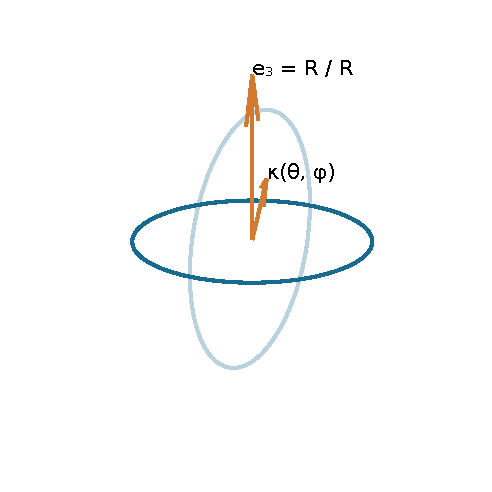
\includegraphics[width=0.55\textwidth]{fourier_sphere}
%\includegraphics[width=0.4\textwidth]{fourierSphere}
\caption{The unit sphere in Fourier space. The unit vector $\bm \kappa(\theta,\phi)$ is defined by the azimuth angle $\phi$, and the  zenith angle $\theta$  measured from the axis $\hat{\bm e}_3=\bm R/R$.}
\label{kSpace}
\end{figure}

In classical  elasticity, the Green's  tensor of the anisotropic Navier operator $G^0_{ij}$ satisfies the following inhomogeneous PDE:
\begin{align}
L_{ik}G^0_{kj}+\delta_{ij}\delta=0\, .
\end{align}
In Fourier space\footnote{
The  Fourier transform  and its inverse are defined as, respectively ~\citep{Wl}:
\begin{align}
\hat{f}(\bm k)=\int_{\mathbb{R}^3} f(\bm x)\, \text{e}^{-\text{i}\bm k\cdot\bm x}\dV\,, &&
f(\bm x)=\frac{1}{(2\pi)^3}\int_{\mathbb{R}^3} \hat{f}(\bm k)\, \text{e}^{\text{i}\bm k\cdot\bm x}\, \text{d}\hat{V}\,.
\end{align}
} this reads:
\begin{align}
\hat{G}^0_{ik}(\bm k)=\frac{1}{k^2}\,\hat{L}^{-1}_{ik}(\bm \kappa)\, .
\end{align}
where $\hat{L}_{ik}(\bm \kappa)=\mathbb{C}_{ijkl}\kappa_j\kappa_l$, $\bm \kappa=\bm k/k$, and $k=\sqrt{\bm k\cdot\bm k}$. The Green's  tensor in real space  is obtained by inverse  Fourier transform. Expressing the elementary volume element in Fourier space as  $\text{d}\hat{V}=k^2\, \text{d}k\, \text{d}\omega$, where $\text{d}\omega$ is an elementary surface element of the unit sphere $\mathcal{S}$, we obtain:
\begin{align}
G^0_{ik}(\bm R)
&=\frac{1}{(2\pi)^3}\int_{\mathbb{R}^3} \frac{\hat{L}^{-1}_{ik}(\bm \kappa)}{k^2}\, \text{e}^{\text{i}\bm k\cdot\bm x} \, \text{d}\hat{V}
=\frac{1}{(2\pi)^3}\int_\mathcal{S}\hat{L}^{-1}_{kl}(\bm \kappa)\, \int_0^\infty \cos(k\bm\kappa\cdot\bm R)\, \text{d}k  \, \text{d}\omega\nonumber
=\frac{1}{8\pi^2R}\int_\mathcal{S}\hat{L}^{-1}_{kl}(\bm \kappa)\, \delta(\bm\kappa\cdot\bm R)  \, \text{d}\omega\, .
\end{align}
Choosing a reference system with $\hat{\bm e}_3$ aligned with $\bm R$, as shown in Fig.~\ref{kSpace}, and using the sifting property of the Dirac $\delta$-function, we finally obtain the expression for the Green tensor as:
\begin{align}
G^0_{ik}(\bm R)= \frac{1}{8\pi^2R}\int_0^{2\pi} \hat{L}^{-1}_{ik}(\bm n)\,  \text{d}\phi\,.
 \label{G0}
\end{align}
Here, $\bm n$ indicates a unit vector on the equatorial plane of the unit sphere in Fourier space. This result was first obtained by \cite{Lifshitz:1947aa} and \cite{Synge:1957aa}.

The classical $\bm F$-tensor, introduced by  \cite{Kirchner:1983}, is defined by Eq. \eqref{F_classical}, which in Fourier space reads:
\begin{align}
\hat{F}^0_{ijkl}=-\hat{G}^0_{kl}\,k_ik_j\,\hGP=-\frac{1}{k^2}\,\hat{L}^{-1}_{kl}(\bm \kappa)\,k_ik_j\, \frac{1}{k^2}=-\frac{1}{k^2}\,\hat{L}^{-1}_{kl}(\bm \kappa)\,\kappa_i\kappa_j\, .
\end{align}
The  classical $\bm F$-tensor in real space is obtained by inverse Fourier transform:
\begin{align}
F^0_{ijkl}(\bm R)&=-\frac{1}{(2\pi)^3}\int_{\mathbb{R}^3}\frac{1}{k^2}\,\hat{L}^{-1}_{kl}(\bm \kappa)\,\kappa_i\kappa_j\, \text{e}^{\text{i}\bm k\cdot\bm R} \, \text{d}\hat{V}
=-\frac{1}{(2\pi)^3}\int_\mathcal{S}\hat{L}^{-1}_{kl}(\bm \kappa)\,\kappa_i\kappa_j\,\, \int_0^\infty \cos(k\bm\kappa\cdot\bm R)\, \text{d}k  \, \text{d}\omega\nonumber\\
&=-\frac{1}{8\pi^2R}\int_\mathcal{S}\hat{L}^{-1}_{kl}(\bm \kappa)\,\kappa_i\kappa_j\, \delta(\bm\kappa\cdot\bm R)  \, \text{d}\omega\, .
\end{align}
In the reference system of Fig.~\ref{kSpace}, we finally obtain:
\begin{align}
F^0_{ijkl}(\bm R)&=-\frac{1}{8\pi^2R}\int_0^{2\pi}\hat{L}^{-1}_{kl}(\bm n)\,n_in_j\,   \, \text{d}\phi\, .
\label{F0}
\end{align}








\chapter{DDD: supplementary derivations}
\begin{draftnote}
This chapter groups the earlier disconnected notes with the DDD theory. The distributional manipulations are retained for review. The uniform-controller algebra is useful for DDD loading, although its current implementation belongs to ElasticDeformation (Chapter~\ref{chap:elastic}).
\end{draftnote}
\section{Kunin identity}
see Berdichevsky, Victor: Variational Principles of Continuum Mechanics: I. Fundamentals, 2009. p.239.
\begin{align}
\int\varphi(\bm x)e^{jkl}\frac{\partial}{\partial x_k}\int_\mathcal{S} \delta(\bm x-\bm x')\hat{n}_ldS'dV&=\int_\mathcal{S} \int\varphi(\bm x)e^{jkl}\frac{\partial}{\partial x_k}\delta(\bm x-\bm x')\hat{n}_ldVdS'\nonumber\\
&=-\int_\mathcal{S} \int\frac{\partial\varphi}{\partial x_k}(\bm x)e^{jkl}\delta(\bm x-\bm x')\hat{n}_ldVdS'\nonumber\\
&=-\int_\mathcal{S} \frac{\partial\varphi}{\partial x_k}(\bm x')e^{jkl}\hat{n}_ldS'\nonumber\\
\end{align}


\section{Distributional identities for loop fields}

Now, since 
\begin{align}
\delta(R)=-\frac{1}{4\pi}\nabla^2\left(\frac{1}{R}\right)=-\frac{1}{8\pi}\nabla^2(R_{,pp})=-\frac{1}{8\pi}R_{,ppqq}
\end{align}
then:
\begin{align}
\beta^p_{kl}(\bm x')=\frac{b_k}{8\pi}\int_\mathcal{S} R_{,ppqq}\hat{n}_ldS''
\label{plasticStrainRderivative}
\end{align}



Consider the derivative of the solid angle using eq.~(\ref{KelvinStokesCorollary})
\begin{align}
\Omega_{,j}=-\frac{1}{2}\int R_{,ppkj}\hat{n}_kdS&=-\frac{1}{2}\int R_{,ppkk}\hat{n}_jdS-\frac{1}{2}\oint\epsilon_{mkj}R_{,ppk}\xi_mdl
\end{align}
then, from eq.~(\ref{plasticStrainRderivative})
\begin{align}
-\frac{b_i}{4\pi}\Omega_{,j}&=\frac{b_i}{8\pi}\int R_{,ppkk}\hat{n}_jdS+\frac{b_i}{4\pi}\oint\epsilon_{kjm}R_{,ppk}\xi_mdl\nonumber\\
&=\beta^p_{ij}+\frac{b_i}{4\pi}\oint\epsilon_{kjm}R_{,ppk}\xi_mdl
\end{align}

\section{Uniform loading: retained derivation}\label{sec:legacycontroller}


The original loading notes describe a uniform controller used to apply a uniform external stress state to the dislocations in the RVE.  The RVE is assumed to be subjected to two loads, an applied stress $\bm \sigma_0$, and a stress $\bm \sigma_s$ exerted by a ``multiaxial spring". Assuming Voigt notation throughout, the spring has \emph{diagonal} stiffness $\bm D$, and it is under an applied strain $\bm \varepsilon_0$, so that $\bm \sigma_s=\bm D\left(\bm \varepsilon_0-\bm\varepsilon\right)$, where $\bm\varepsilon$ is the strain in the RVE. 
Therefore the stress in the RVE is
\begin{align}
\bm \sigma=\bm \sigma_0+\bm \sigma_s= \bm \sigma_0+\bm D\left(\bm \varepsilon_0-\bm\varepsilon\right)
\label{ULC1}
\end{align} 
On the other hand, the RVE stress $\bm \sigma$ is  related to the RVE strain $\bm \varepsilon$ by the relation
\begin{align}
\bm \sigma=\bm C\left(\bm \varepsilon-\bm\varepsilon_p\right)
\label{ULC2}
\end{align} 
where $\bm C$ is the material stiffness, and $\varepsilon_p$ is the plastic strain in the RVE. From \eqref{ULC1} and \eqref{ULC2}, we see that the RVE strain is
\begin{align}
\bm \varepsilon&=\left(\bm C+\bm D\right)^{-1} \left[\bm \sigma_0+\bm D\bm \varepsilon_0+\bm C\bm\varepsilon_p\right]
\end{align}
while the RVE stress is
\begin{align}
\bm \sigma&=\bm C\left(\bm C+\bm D\right)^{-1} \left[\bm \sigma_0+\bm D\left(\bm \varepsilon_0- \bm\varepsilon_p\right)\right]\nonumber\\
\end{align}

We take the diagonal values of $\bm D$ to be $D_i=\alpha_i C_{ii}$ (no summation over $i$), where $\alpha_i$ is an array called ``\emph{machine stiffness ratio}". To understand the effects of the machine stiffness ratio, consider the two limits of small and large $\{\alpha_i\}$'s.

First, suppose that $\alpha_i=0$ for some $i$. Let us rewrite stress as
\begin{align}
\bm \sigma&=\underbrace{\left(\bm I+\bm D\bm C^{-1}\right)^{-1}}_{\bm A}\bm \sigma_0+\underbrace{\left(\bm I+\bm D\bm C^{-1}\right)^{-1}\bm D}_{\bm B}\left(\bm \varepsilon_0- \bm\varepsilon_p\right)
\end{align}
 Note that the $i$-th row of the matrix $\bm I+\bm D\bm C^{-1}$ has a 1 in position $i$ and zeros everywhere else. This implies that also the $i$-th row of the matrix $\bm A$ has a 1 in position $i$ and zeros everywhere else, and in turn that  the $i$-th row of $\bm B$ is zero. This means $\sigma_{i}= \sigma_{0i}$. In other words, setting the $i$-th component of the machine stiffness ratio to zero implies that the corresponding stress component $\sigma_{i}$  matches the applied stress component $\sigma_{0i}$.

Next, consider $\alpha_i\rightarrow\infty$ for some $i$. Let us rewrite strain as
\begin{align}
\bm \varepsilon=\underbrace{\left(\bm I+\bm D^{-1}\bm C\right)^{-1}\bm D^{-1}}_{\bm E} \left[\bm \sigma_0+\bm C\bm\varepsilon_p\right]
+\underbrace{\left(\bm I+\bm D^{-1}\bm C\right)^{-1}}_{\bm F} \bm \varepsilon_0
\end{align}
Here we simply note that the matrices $\bm E$ and $\bm F$ behave similar to the matrices $\bm B$ and $\bm A$ above, respectively. Hence the  $\varepsilon_{i}= \varepsilon_{0i}$. In other words, setting the $i$-th component of the machine stiffness ratio to $\infty$ implies that the corresponding strain component $\varepsilon_{i}$  matches the applied strain component $\varepsilon_{0i}$.
%where $\bm D=\text{diag}{\{D_i\}}$ is a \emph{diagonal} matrix of ``machine stiffness ratios". With this choice we obtain
%\begin{align}
%\bm \varepsilon=\bm C^{-1}\left(\bm I+\bm D\right)^{-1} \left(\bm \sigma_0+\bm C\bm D\bm \varepsilon_0+\bm C\bm\varepsilon_p\right)
%\end{align}
%\begin{align}
%\bm \sigma=\left(\bm I+\bm D\right)^{-1} \bm \sigma_0 + \left(\bm I+\bm D\right)^{-1} \bm D\bm C \left(\bm \varepsilon_0- \bm\varepsilon_p\right)
%\end{align}

%\begin{align}
%\bm \varepsilon=\bm C^{-1}\left(\bm I+\bm D\right)^{-1}\left[\bm \sigma_0+\bm D\bm \varepsilon_0+\bm C\bm\varepsilon_p\right]
%\end{align}

%Method 2
%Now, we assume that $\bm D=\bm C\bm D$, where $\bm D=\text{diag}{\{D_i\}}$ is a \emph{diagonal} matrix of ``machine stiffness ratios". With this choice we obtain
%\begin{align}
%\bm \sigma=\bm C\left(\bm I+\bm D\right)^{-1}\bm C^{-1} \left[\bm \sigma_0+\bm C\bm D\left(\bm \varepsilon_0- \bm\varepsilon_p\right)\right]
%\end{align}




\chapter{Cluster dynamics: current interface and revision boundary}\label{chap:cd}
Cluster dynamics is kept last because its physical model is expected to change. This chapter records the current architectural connection and user entry points; it does not freeze a new constitutive specification.

\section{Connection to the common architecture}
\code{ClusterDynamics} implements \code{MicrostructureBase}. Its base context and parameter object define species data and numerical resources, and its field queries expose mobile concentrations and immobile-cluster quantities to the other microstructures. DDD climb can consume these concentrations. The container also accepts the CD contribution to average plastic distortion and inelastic displacement rate.

The current spatial model uses the shared FEM infrastructure. Species counts are compile-time parameters \code{MODELIB_CD_MSIZE} and \code{MODELIB_CD_ISIZE}; their values must match the material arrays. The default build uses four mobile components and eight immobile fields. These are implementation choices of this snapshot, not a proposed permanent interface for the revised model.
\sourcefile{include/ClusterDynamics/ClusterDynamics.h}
\sourcefile{include/ClusterDynamics/ClusterDynamicsParameters.h}
\sourcefile{src/ClusterDynamics/ClusterDynamics.cpp}

\section{Current user entry points}
Select \code{ClusterDynamics} in \code{physics}, enable the shared FEM, and use a material and \code{ClusterDynamics.txt} compatible with the build. \code{tutorials/spatialCDtest/} is the entry point for the present spatial model. Coupled climb examples require a compatible DDD selection and species configuration as well.

\section{What to document after the revision}
The final CD chapter should define the new state variables and units first, then the conservation equations, diffusion and reaction operators, boundary conditions, time integration, and coupling to DDD and elastic deformation. Each field's contribution to the common interface must be stated. A completed revision should include mass-balance checks, positivity or admissibility criteria, mesh/time-step convergence, and plots from a reproducible example. Those model-specific derivations and plots are intentionally deferred until the implementation settles.

\bibliographystyle{plainnat}
\bibliography{manual_cited}
\end{document}
